%%%%%%%%%%%%%%%%%%%%%%%%%%%%%%%%%%%%%%%%%
% McMaster Masters/Doctoral Thesis
% LaTeX Template
% Version 2.2 (11/23/15)
%
% This template has been downloaded from:
% http://www.LaTeXTemplates.com
% Then subsequently from http://www.overleaf.com
%
% Version 2.0 major modifications by:
% Vel (vel@latextemplates.com)
%
% Original authors:
% Steven Gunn  (http://users.ecs.soton.ac.uk/srg/softwaretools/document/templates/)
% Sunil Patel (http://www.sunilpatel.co.uk/thesis-template/)
%
% Modified to McMaster format by Benjamin Furman (contact: https://www.xenben/com; Most up
% to date template at https://github.com/benjaminfurman/McMaster_Thesis_Template,
% occasionally updated on Overleaf template page)
%
% Modified for macdown by Antonio Paez; most up to date version at https://github.com/paezha/macdown
%
% License:
% CC BY-NC-SA 3.0 (http://creativecommons.org/licenses/by-nc-sa/3.0/)
%
%%%%%%%%%%%%%%%%%%%%%%%%%%%%%%%%%%%%%%%%%

%----------------------------------------------------------------------------------------
% DOCUMENT CONFIGURATIONS
%----------------------------------------------------------------------------------------

\documentclass[
11pt, % The default document font size, options: 10pt, 11pt, 12pt
oneside, % Two side (alternating margins) for binding by default, uncomment to switch to one side
english, % other languages available
singlespacing, % Single line spacing, alternatives: onehalfspacing or doublespacing
%draft, % Uncomment to enable draft mode (no pictures, no links, overfull hboxes indicated)
%nolistspacing, % If the document is onehalfspacing or doublespacing, uncomment this to set spacing in lists to single
%liststotoc, % Uncomment to add the list of figures/tables/etc to the table of contents
%toctotoc, % Uncomment to add the main table of contents to the table of contents
]{macthesis} % The class file specifying the document structure

%----------------------------------------------------------------------------------------
% Import packages here
%----------------------------------------------------------------------------------------
\usepackage[utf8]{inputenc} % Required for inputting international characters
\usepackage[T1]{fontenc} % Output font encoding for international characters
\usepackage{lastpage} % count pages
\usepackage{lmodern} % could change font type by calling a different package
\usepackage{lscape} % for landscaping pages
% New commands for landscape orientation
\newcommand{\blandscape}{\begin{landscape}}
\newcommand{\elandscape}{\end{landscape}}
%
\usepackage{siunitx} % for scientific units (micro-liter, etc)
\setcounter{tocdepth}{2} % so that only section and sub sections appear in Table of Contents. Remove or set depth to 3 to include sub-sub-sections
\usepackage{amsmath}
\usepackage{amssymb}
%----------------------------------------------------------------------------------------
% Define a blank page
%----------------------------------------------------------------------------------------
\def\blankpage{%
      \clearpage%
      \thispagestyle{empty}%
      \addtocounter{page}{-1}%
      \null%
      \clearpage}

%----------------------------------------------------------------------------------------
% Define a tight list
%----------------------------------------------------------------------------------------
\def\tightlist{}

%----------------------------------------------------------------------------------------
%	Highlight Code Chunks
%----------------------------------------------------------------------------------------
  \usepackage{color}
  \usepackage{fancyvrb}
  \newcommand{\VerbBar}{|}
  \newcommand{\VERB}{\Verb[commandchars=\\\{\}]}
  \DefineVerbatimEnvironment{Highlighting}{Verbatim}{commandchars=\\\{\}}
  % Add ',fontsize=\small' for more characters per line
  \usepackage{framed}
  \definecolor{shadecolor}{RGB}{248,248,248}
  \newenvironment{Shaded}{\begin{snugshade}}{\end{snugshade}}
  \newcommand{\AlertTok}[1]{\textcolor[rgb]{0.94,0.16,0.16}{#1}}
  \newcommand{\AnnotationTok}[1]{\textcolor[rgb]{0.56,0.35,0.01}{\textbf{\textit{#1}}}}
  \newcommand{\AttributeTok}[1]{\textcolor[rgb]{0.13,0.29,0.53}{#1}}
  \newcommand{\BaseNTok}[1]{\textcolor[rgb]{0.00,0.00,0.81}{#1}}
  \newcommand{\BuiltInTok}[1]{#1}
  \newcommand{\CharTok}[1]{\textcolor[rgb]{0.31,0.60,0.02}{#1}}
  \newcommand{\CommentTok}[1]{\textcolor[rgb]{0.56,0.35,0.01}{\textit{#1}}}
  \newcommand{\CommentVarTok}[1]{\textcolor[rgb]{0.56,0.35,0.01}{\textbf{\textit{#1}}}}
  \newcommand{\ConstantTok}[1]{\textcolor[rgb]{0.56,0.35,0.01}{#1}}
  \newcommand{\ControlFlowTok}[1]{\textcolor[rgb]{0.13,0.29,0.53}{\textbf{#1}}}
  \newcommand{\DataTypeTok}[1]{\textcolor[rgb]{0.13,0.29,0.53}{#1}}
  \newcommand{\DecValTok}[1]{\textcolor[rgb]{0.00,0.00,0.81}{#1}}
  \newcommand{\DocumentationTok}[1]{\textcolor[rgb]{0.56,0.35,0.01}{\textbf{\textit{#1}}}}
  \newcommand{\ErrorTok}[1]{\textcolor[rgb]{0.64,0.00,0.00}{\textbf{#1}}}
  \newcommand{\ExtensionTok}[1]{#1}
  \newcommand{\FloatTok}[1]{\textcolor[rgb]{0.00,0.00,0.81}{#1}}
  \newcommand{\FunctionTok}[1]{\textcolor[rgb]{0.13,0.29,0.53}{\textbf{#1}}}
  \newcommand{\ImportTok}[1]{#1}
  \newcommand{\InformationTok}[1]{\textcolor[rgb]{0.56,0.35,0.01}{\textbf{\textit{#1}}}}
  \newcommand{\KeywordTok}[1]{\textcolor[rgb]{0.13,0.29,0.53}{\textbf{#1}}}
  \newcommand{\NormalTok}[1]{#1}
  \newcommand{\OperatorTok}[1]{\textcolor[rgb]{0.81,0.36,0.00}{\textbf{#1}}}
  \newcommand{\OtherTok}[1]{\textcolor[rgb]{0.56,0.35,0.01}{#1}}
  \newcommand{\PreprocessorTok}[1]{\textcolor[rgb]{0.56,0.35,0.01}{\textit{#1}}}
  \newcommand{\RegionMarkerTok}[1]{#1}
  \newcommand{\SpecialCharTok}[1]{\textcolor[rgb]{0.81,0.36,0.00}{\textbf{#1}}}
  \newcommand{\SpecialStringTok}[1]{\textcolor[rgb]{0.31,0.60,0.02}{#1}}
  \newcommand{\StringTok}[1]{\textcolor[rgb]{0.31,0.60,0.02}{#1}}
  \newcommand{\VariableTok}[1]{\textcolor[rgb]{0.00,0.00,0.00}{#1}}
  \newcommand{\VerbatimStringTok}[1]{\textcolor[rgb]{0.31,0.60,0.02}{#1}}
  \newcommand{\WarningTok}[1]{\textcolor[rgb]{0.56,0.35,0.01}{\textbf{\textit{#1}}}}

%----------------------------------------------------------------------------------------
% Handling Citations
%----------------------------------------------------------------------------------------
\usepackage[backend=biber, giveninits=true, doi=false, natbib=true, url=false, eprint=false, style=authoryear, sorting=nyt, maxcitenames=2, maxbibnames=99, uniquename=false, uniquelist=false, dashed=false]{biblatex} % can change the maxbibnames to cut long author lists to specified length followed by et al., currently set to 99.
% package xurl wraps long url in the citations.
\usepackage{xurl}
\DeclareFieldFormat[article,inbook,incollection,inproceedings,patent,thesis,unpublished]{title}{#1\isdot} % removes quotes around title
\renewbibmacro*{volume+number+eid}{%
  \printfield{volume}%
%  \setunit*{\adddot}% DELETED
  \printfield{number}%
  \setunit{\space}%
  \printfield{eid}}
\DeclareFieldFormat[article]{number}{\mkbibparens{#1}}
%\renewcommand*{\newunitpunct}{\space} % remove period after date, but I like it.
\renewbibmacro{in:}{\ifentrytype{article}{}{\printtext{\bibstring{in}\intitlepunct}}} % this remove the "In: Journal Name" from articles in the bibliography, which happens with the ynt
\renewbibmacro*{note+pages}{%
    \printfield{note}%
    \setunit{,\space}% could add punctuation here for after volume
    \printfield{pages}%
    \newunit}
\DefineBibliographyStrings{english}{% clears the pp from pages
  page = {\ifbibliography{}{\adddot}},
  pages = {\ifbibliography{}{\adddot}},
}
\DeclareNameAlias{sortname}{last-first}
\renewcommand*{\nameyeardelim}{\addspace} % remove comma in text between name and date
\addbibresource{bib/thesis.bib} % The filename of the bibliography
\usepackage[autostyle=true]{csquotes} % Required to generate language-dependent quotes in the bibliography

% you'll have to play with the citation styles to resemble the standard in your field, or just leave them as is here.
% or, if there is a bst file you like, just get rid of all this biblatex stuff and go back to bibtex.

% This code is to fix cslreferences in new pandoc see: https://github.com/mpark/wg21/issues/54
%%\newlength{\cslhangindent}
%\setlength{\cslhangindent}{1.5em}
%\newenvironment{CSLReferences}%
%  {}%
%  {\par}
%
% https://github.com/ismayc/thesisdown/issues/133
% From {rticles}
% definitions for citeproc citations
\NewDocumentCommand\citeproctext{}{}
\NewDocumentCommand\citeproc{mm}{%
\begingroup\def\citeproctext{#2}\cite{#1}\endgroup}
\makeatletter
% allow citations to break across lines
\let\@cite@ofmt\@firstofone
% avoid brackets around text for \cite:
\def\@biblabel#1{}
\def\@cite#1#2{{#1\if@tempswa , #2\fi}}
\makeatother
\newlength{\cslhangindent}
\setlength{\cslhangindent}{1.5em}
\newlength{\csllabelwidth}
\setlength{\csllabelwidth}{3em}
\newenvironment{CSLReferences}[2] % #1 hanging-indent, #2 entry-spacing
{\begin{list}{}{%
	\setlength{\itemindent}{0pt}
	\setlength{\leftmargin}{0pt}
	\setlength{\parsep}{0pt}
	% turn on hanging indent if param 1 is 1
	\ifodd #1
	\setlength{\leftmargin}{\cslhangindent}
	\setlength{\itemindent}{-1\cslhangindent}
	\fi
	% set entry spacing
	\setlength{\itemsep}{#2\baselineskip}}}
{\end{list}}
\usepackage{calc}
\newcommand{\CSLBlock}[1]{\hfill\break\parbox[t]{\linewidth}{\strut\ignorespaces#1\strut}}
\newcommand{\CSLLeftMargin}[1]{\parbox[t]{\csllabelwidth}{\strut#1\strut}}
\newcommand{\CSLRightInline}[1]{\parbox[t]{\linewidth - \csllabelwidth}{\strut#1\strut}}
\newcommand{\CSLIndent}[1]{\hspace{\cslhangindent}#1}

%----------------------------------------------------------------------------------------
% Collect all your header information from the chapters here, things like acronyms, custom commands, necessary packages, etc.
%----------------------------------------------------------------------------------------
\usepackage{parskip} %this will put spaces between paragraphs
\setlength{\parindent}{15pt} % this will create and indent on all but the first paragraph of each section.
% should maybe change to glossaries package
\usepackage{acro}
\DeclareAcronym{est}{
	short = EST,
	long  = expressed sequence tags
}

\DeclareAcronym{Xl}{
	short = \textit{X.~laevis},
	long  = \textit{Xenopus~laevis}
}
\DeclareAcronym{Xg}{
	short = \textit{X.~gilli},
	long  = \textit{Xenopus~gilli}
}

\usepackage{etoolbox}
\preto\chapter{\acresetall} % resets acronyms for each chapter

\usepackage{xspace} %helps spacing with custom commands.
\newcommand{\oddname}{{\sc SoME goOfY LonG ThiNg With an AwkWarD NAme}\xspace}


\usepackage{pgfplotstable} % a much better way to handle tables
\pgfplotsset{compat=1.12}

 \usepackage{caption}
 \usepackage{float}
 
 \usepackage{booktabs}
\usepackage{caption}
\usepackage{longtable}
\usepackage{colortbl}
\usepackage{array}
\usepackage{xcolor} % Ensure this is included for color support

% if you need to demand figure/table placement, then this will allow you to use [H], which demands a figure placement. Beware, making LaTeX do things it doesn't want may lead to oddities.


%%%%
% LINK COLORS
% You can control the link colors at the end of the McMasterThesis.cls file. There is also a true/false option there to turn off all link colors.
%%%%


%----------------------------------------------------------------------------------------
%	THESIS INFORMATION
%----------------------------------------------------------------------------------------

\title{Inferring the time-varying transmission rate and effective reproduction number by fitting semi-mechanistic compartmental models to incidence data}
%\thesistitle{Thesis Title} % Your thesis title, print it elsewhere with \ttitle
\author{Greg Forkutza}
%\author{John \textsc{Smith}} % Your name, print it elsewhere with \authorname
\bdegree{B.Sc.}
\mdegree{M.Sc.}
%Previous degrees % print it elsewhere with \bdeg and \mdeg
\date{}
% The month and year that you submit your FINAL draft TO THE LIBRARY (May or December)
\university{McMaster University}
%\university{\href{http://www.mcmaster.ca/}{McMaster University}} % Your university's name and URL, print it elsewhere with \univname
%\division{}
\faculty{Faculty of Science} % Your faculty's name and URL, print it elsewhere with \facname
\department{Mathematics \& Statistics} % Your department's name and URL, print it elsewhere with \deptname
\subject{Statistics} % Your subject area, print it elsewhere with \subjectname
%\group{\href{http://researchgroup.university.com}{Research Group Name}} % Your research group's name and URL, print it elsewhere with \groupname
\supervisor{Benjamin Bolker}
%\supervisor{Dr. Jane \textsc{Smith}} % Your supervisor's name, print it elsewhere with \supname
\examiner{} % Your examiner's name, print it elsewhere with \examname
\degree{Master of Science}
%\degree{Doctor of Philosophy} % Your degree name, print it elsewhere with \degreename
\addresses{} % Your address, print it elsewhere with \addressname
\keywords{} % Keywords for your thesis, print it elsewhere with \keywordnames


% this sets up hyperlinks
\hypersetup{pdftitle=\ttitle} % Set the PDF's title to your title
\hypersetup{pdfauthor=\authorname} % Set the PDF's author to your name
\hypersetup{pdfkeywords=\keywordnames} % Set the PDF's keywords to your keywords

\begin{document}
\sloppy

\frontmatter % Use roman page numbering style (i, ii, iii, iv...) for the pre-content pages

\pagestyle{plain} % Default to the plain heading style until the thesis style is called for the body content

%----------------------------------------------------------------------------------------
%	Half Title (lay title)
%----------------------------------------------------------------------------------------
%\begin{halftitle} % could not get this environment working
%\vspace*{\fill}
\vspace{6cm}
\begin{center}
\ttitle
\end{center}
%\vspace*{\fill}
\pagenumbering{gobble} % leave this here, McMaster doesn't want this page numbered
%\end{halftitle}
\clearpage

%----------------------------------------------------------------------------------------
%	TITLE PAGE
%----------------------------------------------------------------------------------------
\pagenumbering{gobble}
\begin{center}

\vfill
\textsc{\Large \ttitle} \\

\vfill
{By \authorname\, \bdeg \, \mdeg }


 \vfill
{\large \textit{A Thesis Submitted to the School of Graduate Studies in the Partial Fulfillment of the Requirements for the Degree \degreename}}\\

\vfill
{\large \univname\, \copyright\, Copyright by \authorname\, \today}\\[4cm] % replace \today with the submission date

\end{center}
\blankpage
\clearpage

%----------------------------------------------------------------------------------------
%	QUOTATION PAGE
%----------------------------------------------------------------------------------------

\vspace*{0.2\textheight}

\noindent{\itshape ``What is your aim in Philosophy?

To show the fly the way out of the fly-bottle.''}\bigbreak

\hfill\textemdash Ludwig Wittgenstein

\blankpage
\clearpage

%%%%%%%%%%%%%%%%%%%%%%%%%%%
%%%%%%%%%%%%%%%%%%%%%%%%%%%
% optional page stuff
%----------------------------------------------------------------------------------------
% can do physical constraints and symbols pages, see the original thesis example on overleaf if you want to include them at https://www.overleaf.com/latex/templates/template-for-a-masters-slash-doctoral-thesis/mkzrzktcbzfl#.VlPeicorpE4
%----------------------------------------------------------------------------------------

%----------------------------------------------------------------------------------------
%	DEDICATION
%----------------------------------------------------------------------------------------


\blankpage
\clearpage


%----------------------------------------------------------------------------------------
%	Descriptive note numbered ii
%----------------------------------------------------------------------------------------
% Need to add below info
\newpage
\pagenumbering{roman} % leave to turn numbering back on
\setcounter{page}{2} % leave here to make this page numbered ii, a Grad School requirement

\noindent % stops indent on next line
\univname \\
\degreename\, (\the\year) \\
Hamilton, Ontario (\deptname) \\[1.5cm]
TITLE: \ttitle \\
AUTHOR: \authorname\,  %list previous degrees
(\univname)  \\
SUPERVISOR: \supname\, \\
NUMBER OF PAGES: \pageref{lastoffront}, \pageref{LastPage}  % put in iv and number

\clearpage

%----------------------------------------------------------------------------------------
%	Lay abstract number iii
%----------------------------------------------------------------------------------------
% not actually included in most theses, though requested by the GSA
% uncomment below lines if you want to include one
\section*{Lay Abstract}
  This thesis explores a new way to model how diseases spread using a deterministic mathematical framework. We focus on estimating the changing transmission rate and the effective reproduction number, key factors in understanding and controlling disease outbreaks. Our method, incorporated into the \texttt{macpan2} software, uses advanced techniques to estimate these changing rates over time. We first prove the effectiveness of our approach with simulations and then apply it to real data from Scarlet Fever, COVID-19, and Measles. We also compare the model performance. Our results show that this flexible and user-friendly approach is a valuable tool for modelers working on disease dynamics.
\blankpage
\clearpage


%----------------------------------------------------------------------------------------
%	ABSTRACT PAGE number iv
%----------------------------------------------------------------------------------------

\section*{\Huge Abstract}
\addchaptertocentry{\abstractname}
% Type your abstract here.
This thesis presents a novel approach to ecological dynamic modeling using non-stochastic compartmental models. Estimating the transmission rate (\(\beta\)) and the effective reproduction number (\(R_t\)) is essential for understanding disease spread and guiding public health interventions. We extend this method to infectious disease models, where the transmission rate varies dynamically due to external factors. Using Simon Wood's partially specified modeling framework, we introduce penalized smoothing to estimate time-varying latent variables within the \texttt{R} package \texttt{macpan2}. This integration provides an accessible tool for complex estimation problems. The efficacy of our approach is first validated via a simulation study and then demonstrated with real-world datasets on Scarlet Fever, COVID-19, and Measles. We infer the effective reproduction number (\(R_t\)) using the estimated \(\beta\) values, providing further insights into the dynamics of disease transmission. Model fit is compared using the Akaike Information Criterion (AIC), and we evaluate the performance of different smoothing bases derived using the \texttt{mgcv} package. Our findings indicate that this methodology can be extended to various ecological and epidemiological contexts, offering a versatile and robust approach to parameter estimation in dynamic models.
\blankpage
\clearpage

%----------------------------------------------------------------------------------------
%	ACKNOWLEDGEMENTS
%----------------------------------------------------------------------------------------

  \begin{acknowledgements}
  \addchaptertocentry{\acknowledgementname} % Add the acknowledgments to the table of contents
    I would like to thank my supervisor, Dr.~Benjamin Bolker. Your mentoring, guidance, and support made this experience enjoyable and rewarding. Thank you for continuously pushing me to become a better statistician and a better programmer. I have grown tremendously because of working with you on this project.

    I would like to thank the faculty and staff within the Department of Mathematics and Statistics at McMaster University. I would like to thank Dr.~Anastasios Kratsios and Dr.~Jonathan Dushoff for participating in my examination committee. I would also like to thank all of the professors I took classes from; it has been a privilege to learn from you all. Lastly, I would like to thank the department staff for always being friendly, helpful, and quick to respond.

    I would like to thank my friends and office mates for their company and for taking the time to talk about research. I would like to thank my two dearest friends in the department, Abhiroop Chowdhury and Manan Mukherjee, for their endless conversations about all things statistics, mathematics, research, philosophy, and art.

    Lastly, I would like to thank my partner, Melanie, for her endless support, patience, love and encouragement. I could not have done this without you.
  \end{acknowledgements}
\blankpage
\clearpage

%----------------------------------------------------------------------------------------
%	LIST OF CONTENTS/FIGURES/TABLES PAGES
%----------------------------------------------------------------------------------------

\tableofcontents % Prints the main table of contents

\listoffigures % Prints the list of figures

\listoftables % Prints the list of tables

%----------------------------------------------------------------------------------------
%	ABBREVIATIONS
%----------------------------------------------------------------------------------------
% many theses don't use this section, as it will be declared at first use and again each chapter. Uncomment these four lines to activate if you want
%\clearpage
%\section*{\Huge Acronyms}
%\addchaptertocentry{Acronyms}
%\printacronyms[name] % name without an option stops the header



%----------------------------------------------------------------------------------------
% The following bit is just here to make sure we end up on a new page and get the total number of roman numeral
\label{lastoffront}
\clearpage
% make sure this command is on the last of your frontmatter pages, i.e. only this command, a \clearpage then \mainmatter
% should be fine without modification
%----------------------------------------------------------------------------------------

%----------------------------------------------------------------------------------------
%	THESIS MAIN BODY
%----------------------------------------------------------------------------------------

\mainmatter % here the regular arabic numbering starts
\pagestyle{thesis}
\chapter{Introduction}\label{introduction}

Ecological dynamic models describe how ecological processes drive populations to change over time by estimating the parameters of the deterministic process, observation error, and process error from a single time series {[}1{]}. However, estimating parameters for dynamic models is challenging. One simplification is to assume that the dynamic model only has observation error, which can be implemented by starting with the initial conditions of the system and computing the entire trajectory over the domain at once. This approach assumes there is no uncertainty in the predicted values of the states at each time step, meaning there is no process error. Since the trajectory at every time step is determined solely by the starting parameters and initial conditions, the model is deterministic. The only error accounted for is the difference between observed and predicted values.

To fit the model to data and compute the maximum likelihood estimate (MLE) for a given set of parameters, one assumes independent observations and sums the likelihood for each observation based on the chosen model of observation error. Using a quasi-Newton method, parameter estimates are updated basek on the current iteration of trajectory matching until convergence is achieved. If the observation error is normally distributed with constant variance, this process simplifies to least squares fitting.

In modeling infectious diseases, for example, one may be interested in estimating the unobserved process of the transmission rate between an infectious individual and a susceptible one. Assuming a fixed value for the transmission rate at every time step is often inaccurate because many diseases have dynamic transmission rates influenced by factors such as seasonality or non-pharmaceutical interventions (e.g., social distancing, masking, and changes in mobility patterns). Therefore, it is reasonable to assume that the transmission rate is a time-varying parameter, computed at each observed data point.

A standard method for dealing with time-varying parameters is to introduce a parametric model and estimate its parameters as part of the MLE process. However, imposing a particular shape on the unknown function describing the unobserved process, is often a phenomenological characterization rather than one derived from known biological mechanisms. This can lead to mismatches between the model and data not due to biological inaccuracies but due to the chosen parametric form of the latent variable.

Fitting dynamic ecological models with time-varying latent variables is a challenging task. Rather than specifying the functional form of the unknown function \emph{a priori}, we can adopt a more flexible function estimation method that minimizes incidental assumptions and model misspecification. {[}2{]} and {[}3{]} developed methodologies for general non-parametric statistical modeling, which have been applied to ecological modeling. Wood and Nisbet {[}4{]} used flexible spline models in population ecology modeling. Ellner et al. {[}5{]} described how to infer information about underlying or unobserved processes in a dynamical system using only time series data. Ellner et al. {[}6{]} introduced the concept of ``semimechanistic'' models, which combine deterministic specifications and parametric models for components supported by known biological mechanisms with non-parametric methods for flexible function estimation when insufficient information is available to justify a specific parametric form. Simon Wood {[}7{]} presented a general methodology using penalized smoothing to estimate time-varying latent variables for dynamic ecological models through iterations of quasi-Newton methods with generalized cross-validation.

Implementing Wood's methodology requires expertise in statistical inference, non-linear optimization, splines, numerical analysis, and statistical computing, making it complex for many domain-specific modelers. Our goal was to develop a user-friendly way for modelers to estimate time-varying latent variables in non-stochastic compartmental models. We integrated Simon Wood's methodology for smoothing parameter estimation into the general-purpose compartmental modeling tool \texttt{macpan2}, which uses \texttt{TMB} for optimization. We use the \texttt{mgcv} package in R to obtain low-rank smoothing matrices for the basis and penalty, resulting in a software module within \texttt{macpan2} that allows users to easily formulate and fit semi-mechanistic models.

Being able to quickly and easily estimate the transmission rate at each observation is crucial for infectious disease modelers. The transmission rate is integral to calculating other epidemiological quantities, such as the effective reproduction number (\(R_t\)), and provides the basis for many downstream applications, including evaluating intervention strategies, forecasting disease dynamics, identifying high-risk periods and populations, validating models, understanding transmission dynamics, assessing the impact of variants, and developing and testing hypotheses about factors influencing disease spread.

In Chapter \ref{Background}, we review the basic theory of univariate smoothing in the context of Gaussian regression and fitting compartmental models to data. We discuss the construction of linear smoothers, review different bases available in the R package \texttt{mgcv}, explore general penalized likelihood methods, and examine the relationship between smooths and random effects, including a Bayesian perspective. Chapter \ref{Materials-and-methods} covers the technical details required to implement the smoothing parameter estimation methodology in \texttt{macpan2}. Chapter \ref{Results} presents the results of the simulation study and applications to Scarlet Fever, COVID-19, and Measles datasets. Finally, Chapter \ref{Discussion} discusses the results, the assumptions and simplifications used in our modeling methodology, and future research avenues.

\chapter{Background}\label{Background}

This chapter contains two sections. The first section outlines the theory required to understand how to use univariate Gaussian regression smoothers in statistical modeling. It finishes by describing the relationship between Gaussian random effects and smoothing splines within a Bayesian framework, which is crucial for fitting semi-mechanistic models to data.

The second section provides a brief introduction to the basic concepts of using compartmental models in the statistical modeling of infectious diseases.

\section{Smoothers}\label{Smoothers}

Linear model methods make the assumption that the true function \(f(x)\) is linear in \(x\). To extend beyond this linearity, one approach is to employ a linear transformation of \(\mathbf{X}\). This leads to:

\[
f(x) = \sum_{m=1}^{M}\beta_m h_m(x),
\]
which is a linear basis expansion of \(x\),
where \(h_m(x): \mathbb{R}^{p} \to \mathbb{R}\) represents the \(m\)-th transformation of \(\mathbf{X}\).

A notable class of these transformations is restriction methods, where the class of functions that \(f(x)\) can assume is limited. A common example within this class is \emph{splines}, which define \(m\) basis functions \(\beta_m h_m(\mathbf{X})\) as local polynomial representations. The domain is divided into contiguous intervals, each represented by a separate polynomial function. The boundaries of these intervals are known as \emph{knots}. An order-\(M\) spline with knots \(\xi_j\), \(j = 1,\dots, K\), is a piecewise-polynomial of order \(M\) and has continuous derivatives up to order \(M-2\).

When the location, derivative order, and number of knots are predetermined, the technique is referred to as regression splines. Natural cubic splines are a specific type where the spline function is composed of cubic polynomial segments.Then it is linear beyond the outermost knots. This spline is represented by \(K\) basis functions \(\beta_m h_m(\mathbf{X})\), one for each specified knot.

The complexity of the fit can be adjusted by incorporating regularization to manage the trade-off between data fidelity and smoothness of the curve fit. This is achieved by minimizing a residual sum of squares with an additional penalty term. The penalty term includes a parameter that controls this trade-off, allowing the fit to range between the extremes of pure interpolation and a linear least squares fit. Splines used in this context are known as smoothing splines.

For a higher-level overview of this topic, see {[}8{]}. For a more detailed exposition, refer to {[}9{]}. Additionally, a comprehensive mathematical treatment of splines and their applications can be found in {[}10{]}.

\subsection{Natural cubic splines}\label{Natural-cubic-splines}

Suppose we have a dataset consisting of points \((x_i, y_i)\) for \(i = 1, \ldots, n\), with each \(x_i\) strictly less than \(x_{i+1}\). A \emph{natural cubic spline} \(g(x)\) is defined as a function that smoothly interpolates between these points. This spline is constructed from cubic polynomial segments, where each segment corresponds to an interval \([x_i, x_{i+1}]\). These polynomial segments are connected such that \(g(x)\), \(g'(x)\), and \(g''(x)\) are all continuous across the entire domain.

Furthermore, the spline satisfies the interpolation condition \(g(x_i) = y_i\) for each point, with the additional constraint that the second derivatives at the endpoints of the domain, \(x_1\) and \(x_n\), are set to zero. This constraint ensures that the spline is linear beyond the boundary points, contributing to its `natural' behavior.

Among all functions that are continuous over \([x_1, x_n]\), possess absolutely continuous first derivatives, and interpolate the given data points \((x_i, y_i)\), the natural cubic spline \(g(x)\) is uniquely the smoothest, meaning that it minimizes the integral:

\begin{equation}
J(f) = \int_{x_{1}}^{x_{2}} f''(x)^{2}\,dx,
\label{eq:min_smoothness}
\end{equation}
which quantifies the overall curvature of the function. Minimizing this integral promotes a function with less curvature and smoother transitions between the interpolated points.

A detailed proof and further discussion on this property of natural cubic splines can be found in {[}11{]}, which explores the mathematical underpinnings and optimizations that define these splines.

\subsection{Cubic smoothing splines}\label{Cubic-smoothing-splines}

With a natural cubic spline, \(g(x)\), we have two main options: we can interpolate the data by setting each \(g(x_i) = y_i\), or we can smooth the data by treating the values \(g(x_i)\) as variables to be optimized, as in \emph{cubic smoothing splines}. Smoothing is achieved by minimizing the following objective function:

\begin{equation}
J_{2}(f) = \sum_{i=1}^n (y_i - g(x_i))^2 + \lambda \int g''(x)^2 \, dx,
\label{eq:min_smoothness_obj}
\end{equation}

Here, \(\lambda\) serves as a tuning parameter that balances the fidelity to the data with the smoothness of the function \(g\). A higher \(\lambda\) value places greater emphasis on minimizing the integral of the squared second derivative, which encourages a smoother curve for \(g\). Conversely, a lower \(\lambda\) value focuses on closely matching the actual data points, minimizing the sum of squared differences \(\sum_{i=1}^n (y_i - g(x_i))^2\).

The formulation given in Equation \ref{eq:min_smoothness_obj} is flexible and does not depend on a predefined set of basis functions. Instead, the model itself dictates the structure, leading to the derivation of optimal basis functions based on the specified terms for data fidelity and smoothness.

Solving Equation \ref{eq:min_smoothness_obj} involves addressing a variational problem in which the basis functions for the cubic spline are obtained using the Euler-Lagrange equation. A detailed derivation of this process can be found in {[}12{]}. However, this derivation is lengthy and involves extensive algebraic manipulation, which can obscure the conceptual foundations of the proof. In Appendix \ref{A1}, we extract and explain key lines from the proof to provide a deeper understanding of why these basis functions take their particular form. We present this outline for two primary reasons: historically, cubic smoothing splines were among the first types of smoothers to be thoroughly investigated. Furthermore, the general approach of penalized likelihood methods can be effectively abstracted from the solution to the minimization problem presented by cubic smoothing splines. For a broader definition of penalized splines, refer to subsection \ref{General-definition-of-a-penalized-spline}

\subsection{Cubic regression splines}\label{Cubic-regression-splines}

Using the results from appendix \ref{A1}, we can define the cubic spline function \(f(x)\) with \(k\) knots \(x_1, \dots, x_k\) as follows:

\begin{equation}
f(x) = a_j(x)f(x_j) + b_j(x_j)f(x_{j+1}) + c_j(x)f''(x_j) + d_j(x_j)f''(x_{j+1}),
\label{eq:spline eqn}
\end{equation}
where \(x_j \leq x \leq x_{j+1}\) and \(a_j, b_j, c_j\) and \(d_j\) are the basis functions of the cubic spline function, derived in Equation \ref{eq:spline_basis_functions}.

This formulation ensures continuity at each knot, as the continuity conditions Equation \ref{eq:continuity_conditions} imply that the derivatives at the knots must match:

\begin{equation}
\mathbf{B} \cdot (f''(x_2),\dots, f''(x_{k-1}))^{T} = \mathbf{D} \cdot (f(x_2),\dots, f(x_{k-1}))^{T},
\label{eq:spline_matrix_equations}
\end{equation}
where \(B\) defines the relationships among the second derivatives and \(D\) defines the relationships between the second derivatives and the function values. \(B\) and \(D\) are therefore the matrix elements expressing the continuity and naturally constraints as defined in Equations \ref{eq: spline_matrix_element_B} and \ref{eq: spline_matrix_element_D}.

By integrating these conditions into Equation \ref{eq:spline eqn}, and redefining \(f(x)\) in terms of the basis functions, we arrive at:

\begin{equation}
f(x) = \sum_{i=1}^{k}b_i(x)\beta_i,
\label{eq:spline sum}
\end{equation}
where \(\beta_i = f(x_i)\) and \(b_i\) represents the transformed basis functions obtained by applying \(\mathbf{B^{-1}D}\) to the original basis functions \ref{eq:spline_basis_functions}. This defines a \emph{cubic regression spline}. The full details of how to derive equation \ref{eq:spline sum} from equation \ref{eq:spline_matrix_equations} can be found in {[}13{]}.

This structure effectively maps the spline basis to the spline evaluated at a specified set of knots. Furthermore, a computationally efficient form of Equation \ref{eq:min_smoothness} in terms of these basis functions and matrix elements is:

\[
\int_{x_1}^{x_k} f''(x)^2 \, dx = \beta^T \mathbf{D}^T \mathbf{B}^{-1} \mathbf{D} \beta =  \beta^T \mathbf{S} \beta,
\]
where \(\mathbf{S} \equiv \mathbf{D}^T \mathbf{B}^{-1} \mathbf{D}\) is the called the \emph{penalty matrix} for this basis.

In subsection \ref{General-definition-of-a-penalized-spline}, we show how the method of penalizing cubic splines lead to a more general method of penalized regression and the abstract notion of penalized likelihood methods.

In the following sections we investigate some other penalized regression splines that are are used in chapter \ref{Results} as smoothers (available as basis and penalty matrices in the R package \texttt{mgcv}) for estimating time-varying parameters in discrete time deterministic compartmental models.

\subsection{B-splines}\label{B-splines}

B-splines offer another basis for representing polynomials that are used in constructing smoothing splines. Detailed explanations of B-spline basis functions and their mathematical properties can be found in {[}8{]} and {[}10{]}. For a concise definition of B-spline basis functions, refer to {[}9{]}.

\emph{B-splines} allow an \((m+1)^{\text{th}}\) order spline to be expressed uniquely using the B-spline basis functions \(B_i^m(x)\):

\[
f(x) = \sum_{i=1}^{k} B_i^m(x) \beta_i,
\]
where each \(B_i^m(x)\) is defined by a local combination of knots. The means any nice curve can be uniquely represented as a linear combination of B-splines and hence as a linear smoother.

\subsection{P-splines}\label{P-splines}

\emph{P-splines} are a low-rank smoother (the number of knots is less than the length of the input vector) that adapt a B-spline basis with a penalty to control wiggliness by penalizing adjacent \(\beta_i = f(x_i)\). The penalty term \(\mathbf{P}\) is defined as:

\[
\mathbf{P} = \sum^{k-1}_{i=1}(\beta_{i+1}-\beta_i)^2.
\]

To express this penalty in matrix form, let \(\mathbf{R}\) be defined as follows:

\[
\mathbf{R} = \begin{bmatrix}
-1 & 1 & 0 & \cdots & 0 \\
0 & -1 & 1 & \cdots & 0 \\
\vdots & & \ddots & \ddots & \vdots \\
0 & \cdots & 0 & -1 & 1 
\end{bmatrix}.
\]

Using this matrix \(\mathbf{R}\), the differences between adjacent \(\beta_i\) can be written as:

\[
\begin{bmatrix}
\beta_2 - \beta_1 \\
\beta_3 - \beta_2 \\
\vdots \\
\beta_k - \beta_{k-1}
\end{bmatrix}
= \mathbf{R} \beta.
\]

The penalty term for adjacent basis coefficients can then be written as:

\[
\mathbf{P} = \beta^T \mathbf{R}^T \mathbf{R} \beta.
\]

When we multiply out \(\mathbf{R}^T \mathbf{R}\), we obtain:

\[
\mathbf{R}^T \mathbf{R} = \begin{bmatrix}
1 & -1 & 0 & \cdots & 0 \\
-1 & 2 & -1 & \cdots & 0 \\
0 & -1 & 2 & -1 & \cdots \\
\vdots & & \ddots & \ddots & \vdots \\
0 & \cdots & 0 & -1 & 1 
\end{bmatrix}.
\]

Thus, the penalty term can be fully expressed as:

\[
\mathbf{P} = \beta^T
\begin{bmatrix}
1 & -1 & 0 & \cdots & 0 \\
-1 & 2 & -1 & \cdots & 0 \\
0 & -1 & 2 & -1 & \cdots \\
\vdots & & \ddots & \ddots & \vdots \\
0 & \cdots & 0 & -1 & 1 
\end{bmatrix}
\beta.
\]

This formulation ensures that the differences between adjacent \(\beta_i\) are penalized, thereby controlling the smoothness of the resulting P-spline.

\subsection{Thin plate regression splines}\label{Thin-plate-regression-splines}

So far, the discussion has focused on smoothing methods that apply to a single predictor variable. While uni variate smoothing is useful, multivariate smoothing techniques available as well. One such technique is the thin plate splines (TPS). We follow the method given by Simon Wood in {[}14{]}.

In the general case, a \emph{thin plate spline} (TPS) is defined for a number of predictor variables \(d\) and a penalty of degree \(m\) such that \(2m > d\). The TPS penalty, \(J_{md}\), is given by:

\[
J_{md} = \int_{\mathbb{R}^d} \sum_{\nu_1 + \cdots + \nu_d = m} \frac{m!}{\nu_1! \cdots \nu_d!} \left( \frac{\partial^m f}{\partial x_1^{\nu_1} \cdots \partial x_d^{\nu_d}} \right)^2 \, dx_1 \cdots dx_d,
\]
where \(\nu_1, \nu_2, \ldots, \nu_d\) are non-negative integers representing the orders of the partial derivatives with respect to each predictor variable \(x_i\).

The function that minimizes this penalty is expressed as:

\[
\hat{f}(x) = \sum_{i=1}^n \delta_i \eta_{md}(\|x - x_i\|) + \sum_{j=1}^M \alpha_j \phi_j(x),
\]
where \(\delta\) and \(\alpha\) are vectors of coefficients to be estimated. The \(\delta\) coefficients must satisfy the linear constraints \(\mathbf{T}^T \delta = 0\), with \(T_{ij} = \phi_j(x_i)\). Here, \(M = \binom{m+d-1}{d}\), representing the number of linearly independent polynomials \(\phi_i(x)\) that span the space of polynomials in \(\mathbb{R}^d\) of degree less than \(m\). These polynomials form the null space of \(J_{md}\).

The remaining basis functions \(\eta_{md}(r)\) are defined as:
\[
\eta_{md}(r) = 
\begin{cases} 
(-1)^{m+1+d/2} \frac{2^{2m-1} \pi^{d/2} (m-1)!}{\Gamma(m-d/2)!} r^{2m-d} \log(r), & \text{if } d \text{ is even}, \\
\Gamma(d/2 - m) \frac{2^{2m} \pi^{d/2} (m-1)!}{\Gamma(m)} r^{2m-d}, & \text{if } d \text{ is odd}.
\end{cases}
\]

Therefore thin plate splines area an expansion of \(\delta_i\) in radial basis functions \(\eta_{md} (r)\).

In the univariate case with derivative penalty of degree two, i.e \(d =  1\) and \(m = 2\), equation \ref{eq: general penalized spline} is equivalent to that of the cubic smoothing spline, with objective function equation \ref{eq:min_smoothness_obj}.

In this case, the minimizing function has the form:
\[
\hat{f}(x) = \sum_{i=1}^n \delta_i |x - x_i|^2 \log(|x - x_i|) + \alpha_0\phi_1(x) + \alpha_1 \phi_2(x),
\]
where the basis function \(\eta_{21}(r) =|x - x_i|^2 \log(|x - x_i|)\) is a specific radial basis function for the univariate TPS. The basis functions \(\phi_i\) are:
\[
\phi_1(x) = 1, \quad \phi_2(x) = x_1.
\]
Here, \(\delta_i\) and \(\alpha_j\) are coefficients to be estimated, with \(\alpha_0\) and \(\alpha_1\) accounting for the polynomial part of the spline, which form the familiar ``linear'' null space of the univariate Gaussian objective function we have seen so far.

The expression of a TPS as a linear mixed model, with a separation of basis functions into null and non-null spaces, shows how the smoothness penalty operates. We construct the model matrix for the basis functions \(\mathbf{E}\) for the radial basis functions \(\mathbf{E}_{ij} = |x_i - x_j|^2 \log(|x_i - x_j|)\) and \(\mathbf{T}\) for the polynomial basis functions \(\mathbf{T}_{ij} = \phi_j(x_i)\). By expressing the function \(\hat{f}(x)\) in terms of \(\delta\) and \(\alpha\), the minimization problem becomes:

\[
\text{minimize} \quad \left\| \mathbf{y} - \mathbf{E} \delta - \mathbf{T} \alpha \right\|^2 + \lambda \delta^T \mathbf{E} \delta \quad \text{subject to} \quad \mathbf{T}^T \delta = 0,
\]
where \(\mathbf{y}\) is the vector of observed data points \(y_i\), \(\mathbf{E} \delta\) captures the non-null space (penalized) part of the basis functions, \(\mathbf{T} \alpha\) captures the null space (unpenalized) part of the basis functions and the constraint \(\mathbf{T}^T \delta = 0\) ensures that the non-null space coefficients \(\delta\) do not interfere with the polynomial terms.

See subsection \ref{The-duality-of-smooths-and-random-effects} for background on thinking about smoothers as random effects in a linear mixed model framework.

Now Simon Wood constructs a low rank version of TPS called \emph{thin plate regression spline} (TPRS) by leaving the \(\mathbf{\alpha}\) parameter space unchanged and instead finding a truncated basis in the \(\mathbf{\delta}\) parameter space. Details of this construction are done in {[}15{]}. TPRS are the low rank approximation to TPS that are used in the R package \texttt{mgcv}, that we use to obtain the basis and penalty matrices for our smoothers. See chapter \ref{Materials-and-methods} for more details on how \texttt{mgcv} is used in constructing compartmental model using smoothers to estimate time varying latent variables.

\subsection{General definition of a penalized spline}\label{General-definition-of-a-penalized-spline}

The penalized regression problem, formulated to minimize:
\begin{equation}
\|y - \mathbf{X}\beta\|^2 + \lambda \beta^T \mathbf{S} \beta,
\label{eq:penalizedregression}
\end{equation}
leads to a solution for the \emph{smoothing coefficients} \(\beta\) expressed as:

\begin{equation}
\hat{\beta} = (\mathbf{X}^T\mathbf{X}+ \lambda \mathbf{S})^{-1}\mathbf{X}^Ty,
\label{eq:penalizedleastsquaresminimizer}
\end{equation}
with the corresponding hat matrix:

\[
\mathbf{A} = \mathbf{X}(\mathbf{X}^T\mathbf{X}+ \lambda \mathbf{S})^{-1}\mathbf{X}^T,
\]
often called the \emph{smoother matrix}. In a typical data model \(y = f(x) + \epsilon\), the estimate \(\hat{y}\) is computed as:

\[
\hat{y} = \mathbf{L}y,
\]
where \(\mathbf{L}\) is an \(n \times n\) matrix dependent on \(\lambda\). Although \(\mathbf{L}\) renders the smoother non-linear in nature due to its dependency on \(\lambda\), it can be treated as linear for fixed \(\lambda\), simplifying the use of penalized regression splines in practical applications.

Now, consider the general case of flexible function estimation within a statistical model defined over the domain \(\mathbb{R}^n\). The functional can be expressed as:

\begin{equation}
S(f) = L(f | \text{data}) + J(f),
\label{eq: general penalized spline}
\end{equation}
where \(L(f | \text{data})\) represents the likelihood of the function \(f\) given the data---essentially the deterministic part of the model---and \(J(f)\) is a functional that defines what it means for functions \(f\) on the domain \(\mathbb{R}^n\) to be smooth.

In the examples discussed previously, such as cubic smoothing splines, P-splines, B-splines, and thin-plate regression splines, each represents a specialized case of this general equation tailored for Gaussian regression. Typically, the data model is assumed to be \(y = f(x) + \epsilon_i\), where \(\epsilon_i\) follows a Gaussian distribution. This assumption gives the likelihood function \(L(f)\) the form of a least squares functional, and the roughness penalty \(J(f)\) the form of a quadratic penalty. This follows from the theory of reproducible kernel Hilbert spaces, which we do not consider further. See Gu {[}16{]} for further details. However, one could alternatively assume a different distribution (e.g., from the exponential family) for the residual errors in the data model, which would modify \(L(f)\) accordingly. The choice of a quadratic functional as the roughness penalty is also based on this assumption. Specializing to Gaussian Regression simplifies equation \ref{eq: general penalized spline} to the specific form seen in equation \ref{eq:min_smoothness_obj}.

By focusing on Gaussian regression within the framework of penalized likelihood estimation, we derive an objective function that integrates both a stochastic component, the least squares functional and a roughness penalty component, the quadratic functional.

\subsection{Emperical Bayes and the duality of smooths and random effects}\label{The-duality-of-smooths-and-random-effects}

In a Bayesian context, prior beliefs about parameters before observing the data are specified through a prior distribution. For smoothing, the penalty term \(\beta^T \mathbf{S} \beta\) suggests a prior on \(\beta\):

\begin{equation}
\beta \sim \mathcal{N}(0, \mathbf{S}^{-}/\lambda),
\label{eq:penalty prior}
\end{equation}
where \(\mathbf{S}^{-}\) is the pseudoinverse of \(\mathbf{S}\), accounting for its rank deficiency. This prior implies that the values of \(\beta\) are normally distributed with a mean of zero and a covariance matrix \(\mathbf{S}^{-}\), tightening around zero as \(\lambda\) increases and becoming flatter as \(\lambda\) decreases. This Bayesian interpretation of smoothing is discussed in {[}9{]}.

Consequently, the maximum posteriori (MAP) estimate of \(\beta\) is given by:
\begin{equation}
\beta \mid y \sim \mathcal{N}(\hat{\beta}, (\mathbf{X}^T \mathbf{X} + \lambda \mathbf{S})^{-1} \sigma^2),
\label{eq:MAP estimate}
\end{equation}
which aligns with the solution of Equation \ref{eq:penalizedleastsquaresminimizer} derived from Equation \ref{eq:penalizedregression}.

This reveals that methodologies designed for smoothing problems are applicable for estimating Gaussian random effects.

It is possible to conceptually link penalized smoothing splines with linear mixed models (LMMs). This connection was first explored in-depth in {[}17{]}. In this framework,the smooth function in flexible function estimation is represented by a high-dimensiona lbasis. The penalty on spline coefficients, represented as \(\beta^T \mathbf{S} \beta\), can be interpreted as an \emph{a priori} distribution, yielding a mixed linear model by treating the smooth components of the model as random effects. The parametric components and the components of the smooth in the null space are treated as fixed effects. For a deep exploration of this duality see {[}2{]} or {[}17{]}. For a computational overview see {[}14{]}.

The primary advantage of using the mixed model formulation for penalized splines is that the computational methods developed to estimate random effects in software like \texttt{lme4} can also be employed to estimate smooth functions. However, it is possible to write the objective function out explicitly with the penalty term expressed as a quadratic form using the penalty matrices computed via the \texttt{mgcv} package. Optimization of the objective function is handled by \texttt{macpan2}, which uses Template Model Builder as the optimization engine {[}18{]}. Therefore in this case it is not necessary to write out the model in the mathematical form of a mixed model. However, should one choose to adopt this modeling methodology with another optimization engine, detailing the model in the form of a mixed model could be essential.

\subsection{Gaussian processes regression smoothers}\label{Gaussian-process-regression-smoothers}

A \emph{random field} is a function \(f\) that assigns a random value \(f(x_i)\) at each point \(x_i\) within its domain \(\mathcal{X}\). If we assume that the collection of values \(f(x)\) for any finite selection of points \(\{x_i\}_{i=1}^n\) follows a multivariate Gaussian distribution, then the subset \(\{f(x_i)\}_{i=1}^n\) is jointly normally distributed. This distribution is characterized by a mean function \(\mu(x)\) and a covariance function \(C(x, x')\), which measures how correlations decay with distance between any two points, thereby defining a \emph{Gaussian Random Field} (GRF).

Unlike being restricted to fixed or discrete locations, a GRF can be generalized by defining a distribution over functions, making the model continuous with respect to its domain. How is this achieved? The covariance function \(C\) of the GRF, initially defined on a set of discrete points such as a lattice, can be generalized through a \emph{kernel} \(k(x, x_i)\). This kernel extends the covariance function to a continuous domain, ensuring that its realization over any finite subset of this domain yields a positive semi-definite matrix. This requirement extends the univariate requirement of a positive variance parameter \(\sigma^2\) to a multivariate scenario.

A \emph{Gaussian process} is thus defined as the model where any finite collection of realizations (i.e., \(n\) observations) is treated as having a multivariate normal distribution. The characteristics of these realizations are determined by the mean function \(\mu(x)\) and the kernel \(k(x, x_i)\), with the latter's realization forming a positive semi-definite symmetric matrix \(\mathbf{K}\).

The function \(f\) can be represented as:
\[
f(x) = (1, \mathbf{x}^T)\beta + \sum_i b_i C(x, x_i),
\]
where \(C(x, x_i)\) is a non-negative function measuring the distance between two points. The value of \(C(x, x_i)\) should equal one when points are identical (indicating maximum correlation) and approach zero as the distance between points increases to infinity. Given the vector \(b\), its prior distribution is \(b \sim \mathcal{N}(0, \mathbf{S}^{-1}/\lambda)\). Here, \(\beta\) is a vector of fixed effect parameters (in the sense of the mixed model formulation), and the model depicts \(f\) as a linear combination of these fixed effects and a random effect weighted by the kernel function \(C(x, x_i)\).

In matrix form, \(f\) is represented as:
\[
f = \mathbf{B} \beta + \mathbf{C}b.
\]
To find the covariance matrix of \(f\), compute:
\[
\text{Cov}(f) = \text{Cov}(\mathbf{C}b) = \mathbf{C} \text{Cov}(b) \mathbf{C}^T = \mathbf{C} (\lambda \mathbf{C})^{-1} \mathbf{C}^T = \mathbf{C} / \lambda,
\]
leveraging the fact that \(C = S^{-1}\) and \(\mathbf{C}\) is symmetric.

Minimizing the objective function:
\[
\|y - \mathbf{B}\beta - \mathbf{C}b\|^2/\sigma^2 + \lambda b^T \mathbf{C} b
\]
is equivalent to maximizing the posterior probability of the parameters given the data, usually incorporating \(\sigma^2\) into the smoothing parameter \(\lambda\). The values of \(\beta\) and \(b\) that minimize this function are the MAP estimates given in equation \ref{eq:MAP estimate}.

This methodology is known as \emph{Gaussian process regression}. Gaussian process regression's complexity primarily resides in the choice of the kernel. The kernel encodes assumptions about the function \(f\) by defining the concept of proximity or similarity used in the estimation. For an introduction to Gaussian Processes, including many covariance functions and further details, see {[}19{]}.

\subsection{Ornstein--Uhlenbeck process}\label{OU}

The Ornstein-Uhlenbeck (OU) process emerges as a special case of the Matérn covariance function with \(\nu = \frac{1}{2}\). This formulation leads to a stationary first-order Gauss Markov process.

The \emph{Matérn class} of covariance functions is a Gaussian processes defined as:
\[
k(r) = \sigma^2 \frac{2^{1-\nu}}{\Gamma(\nu)}\left(\frac{\sqrt{2\nu} r}{\ell}\right)^\nu K_\nu\left(\frac{\sqrt{2\nu} r}{\ell}\right),
\]
where \(r\) is the distance between points, \(\sigma^2\) is the variance, \(\ell\) is the length scale, \(\nu\) is a smoothness parameter and \(K_\nu\) is a modified Bessel function of the second kind.

When \(\nu = \frac{1}{2}\), the Matérn function simplifies significantly because the modified Bessel function of the second kind, \(K_{1/2}(z)\), has a known simple form that relates to the exponential function. The formula for \(K_{1/2}(z)\) is:
\[
K_{1/2}(z) = \sqrt{\frac{\pi}{2z}} e^{-z}.
\]
Substituting \(\nu = \frac{1}{2}\) into the Matérn formula, using \(\Gamma(\frac{1}{2}) = \sqrt{\pi}\), we get:
\[
k(r) = \sigma^2 e^{-r/\ell}.
\]
Here, \(\ell\) acts as a scale parameter, and the resulting covariance function is the exponential covariance function.

The \emph{Ornstein-Uhlenbeck process} is a continuous-time stochastic process that is both Gaussian and Markov, characterized by its mean-reverting property. The covariance function of the OU process over time \(t\) with mean reversion rate \(\theta\) is given by:
\[
k(t) = \sigma^2 e^{-\theta |t|},
\]
where \(\theta > 0\) is the rate at which the process reverts to its mean.

Comparing this with the exponential covariance function derived from the Matérn function, we see that they are essentially the same form when interpreted over time rather than space, with \(\theta = 1/\ell\). Thus, the OU process, which has this exponential form of the covariance function, is a Gaussian Markov process.

Setting \(\nu = \frac{1}{2}\) in the Matérn covariance function yields an exponential covariance function, which corresponds to the covariance structure of the OU process. The first-order Markov property in the OU process is given from the memoryless feature of the exponential decay in its covariance function. This demonstrates how the OU process, as a stationary first-order Gaussian Markov process, is a special case of the Gaussian processes modeled by the Matérn covariance function with \(\nu = \frac{1}{2}\).

\section{Conditional Akaike information criterion}\label{conditional-akaike-information-criterion}

How can we account for overfitting in statistical modeling when comparing the fit of two different models, which incorporate penalization, to data?

See appendix \ref{AIC} for the background on the using \emph{Akaike information criterion} (AIC) for comparison between models with unpenalized parameters. Given equation \ref{eq:AIC}, we now have a measure for model performance that takes into account complexity by penalizing for the number of parameters in the model. However, the notion of degrees of freedom for penalized smoothing coefficients is more complicated than in the unpenalized case. To address this complexity, it is helpful to introduce the concept of natural parameterization and the effective degrees of freedom (EDF). These concepts explain the impact of penalties on model coefficients and for defining a correction notion for what \(p\) should be in expression \ref{eq:AIC}.

In the context of penalized smoothers, Simon Wood {[}9{]} describes a ``natural'' parameterization, that simplifies the understanding of how penalties affect model degrees of freedom. The \emph{natural parameterization} transforms the parameter estimators such that they are independent with unit variance in the absence of a penalty, and the penalty matrix becomes diagonal.

Consider a model with a design matrix \(\mathbf{X}\), parameter vector \(\boldsymbol{\beta}\), wiggliness penalty matrix \(\mathbf{S}\), and smoothing parameter \(\lambda\). Using the QR decomposition, \(\mathbf{X}\) is factorized as \(\mathbf{X} = \mathbf{Q} \mathbf{R}\). Re-parameterizing in terms of \(\boldsymbol{\beta''} = \mathbf{R} \boldsymbol{\beta}\) transforms the model matrix to \(\mathbf{Q}\) and the penalty matrix to \(\mathbf{R}^{-T} \mathbf{S} \mathbf{R}^{-1}\).

The penalty matrix is then eigen-decomposed as \(\mathbf{R}^{-T} \mathbf{S} \mathbf{R}^{-1} = \mathbf{U} \mathbf{D} \mathbf{U}^T\), where \(\mathbf{U}\) is orthogonal and \(\mathbf{D}\) is diagonal. Further re-parameterization via a rotation/reflection of the parameter space yields parameters \(\boldsymbol{\beta'} = \mathbf{U}^T \boldsymbol{\beta''}\), resulting in a model matrix \(\mathbf{Q} \mathbf{U}\) and penalty matrix \(\mathbf{D}\). This ``natural'' parameterization allows for a clear understanding of the penalty's role in limiting parameter variance.

Each unpenalized coefficient has one degree of freedom. The penalized estimates are shrunken versions of the unpenalized estimates: \(\hat{\beta'}_i = (1 + \lambda D_{ii})^{-1} \tilde{\beta'}_i\), where \(D_{ii}\) are the eigenvalues of the penalty matrix. The shrinkage factor \((1 + \lambda D_{ii})^{-1}\) represents the \emph{effective degrees of freedom} for each penalized coefficient.

The total EDF for the smooth is the sum of the individual shrinkage factors:

\[
\sum_i (1 + \lambda D_{ii})^{-1} = \text{tr}(\mathbf{\tau}) \quad \text{where} \quad \mathbf{\tau} = (\mathbf{X}^T \mathbf{X} + \lambda \mathbf{S})^{-1} \mathbf{X}^T \mathbf{X}.
\]

\(\tau\) can be interpreted as the matrix that maps the un-penalized coefficient estimates to the penalized coefficient estimates. This means that the trace of \(\tau\) can be understood as having the effect of being the average shrinkage of the coefficients, multiplied by the number of coefficients. This measure is bounded between the number of zero eigenvalues of the penalty (as \(\lambda \to \infty\)) and the total number of coefficients (when \(\lambda = 0\)). The `trace of the hat matrix' is an idea also found elsewhere, e.g Hastie et Tibshirani {[}8{]}.

The unpenalized estimators are unbiased, leading to the expected value of the penalized estimates: \(E(\hat{\beta'}_i) = (1 + \lambda D_{ii})^{-1} \beta_i\). The shrinkage factors determine the relative smoothing bias.

The penalty suppresses variability in parameters corresponding to high eigenvalues \(D_{ii}\), effectively reducing model complexity.

Therefore, the AIC formula corrected to incorporate the effective degrees of freedom is the \emph{conditional AIC}:

\begin{equation}
\text{AIC} = -2 \ell(\hat{\beta}) + 2 \tau.
\label{eq:corrected AIC}
\end{equation}

The effective degrees of freedom for the calibrated models are computed as the model degrees of freedom, facilitating the comparison of models using different smoothing bases with the same data set, as in Chapter \ref{Results}.

Although the model degrees of freedom take into account the value of the smoothing parameter, it does not take into account the uncertainty estimates of the fitted smoothing parameter. From Appendix \ref{AIC}, the effective degrees of freedom is equal to:

\[
\tau = \text{tr}2\mathbb{E}\left[\frac{1}{2} (\hat{\beta} - \beta_K)^T \mathbf{ \mathcal{I}}_K (\hat{\beta} - \beta_K)\right] = \text{tr}  \mathbb{E}[\chi^2_p] = p,
\]
where \(\beta_K\) is the coefficient vector minimizing the K-L divergence and \(\mathbf{ \mathcal{I}}_K\) is the expected negative Hessian of the log likelihood. In {[}20{]}, Wood et al defines the corrected AIC as

\[
\tau_2 = \text{tr}(\mathbf{V}'_{\beta}\hat{\mathbf{ \mathcal{I}}}),
\]
where \(\mathbf{V}'\) is an approximation of the covariance matrix of the Bayesian large sample approximation

\[
\beta \mid y,\lambda \sim \mathcal{N}(\hat{\beta}_{\lambda},\mathbf{V}_{\beta})
\]
and \(\mathbf{V}_{\beta} = (\hat{\mathbf{\mathcal{I}}} + \mathbf{P})^{-1}\). \(\hat{\mathbf{ \mathcal{I}}}\) is the is the Hessian of the negative log likelihood at \(\mathbf{ \mathcal{I}}_K\). The goal is to calculate a first-order adjustment to the posterior distribution of the model coefficients, taking into account the uncertainty in the smoothing parameter. After that, the penalty term in the AIC is represented using the Bayesian covariance matrix of the coefficients.

\section{The SIR and SIRS compartmental models}\label{the-sir-and-sirs-compartmental-models}

The \emph{SIR model} (Figure \ref{fig:sir-model}) categorizes the population into three distinct compartments: \(S(t)\), \(I(t)\), and \(R(t)\), which represent the number of susceptible, infected, and recovered individuals, respectively. As the disease progresses, the number of individuals in each compartment changes over time, thus these compartments are represented as functions of time. The transitions between these compartments are guided by the processes depicted in the schematic shown in Figure \ref{fig:sir-model}.

The model incorporates two primary parameters: the transmission rate (\(\beta\)) and the recovery rate (\(\gamma\)). The \emph{transmission rate}, \(\beta\) is the per capita rate at which two different individuals come in effective contact per unit time. This rate is used to calculate \(\beta SI\), where \(SI\) is the total number of interactions between susceptible and infected individuals; \(\beta SI\) thus represents the expected number of new infections per unit time.

On the other hand, the \emph{recovery rate}, \(\gamma\), indicates how quickly infected individuals recover and gain immunity. If an individual is infectious for a period \(D\), then \(\gamma\) is defined as \(\gamma = \frac{1}{D}\). Therefore, \(\gamma I\) calculates what proportion of the infected population will recover during any given time interval, moving from the infected compartment to the recovered compartment, based on the infectious period \(D\).

\begin{figure}[H]
\centering
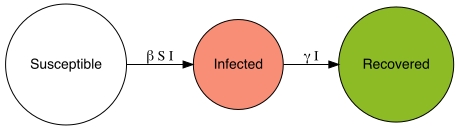
\includegraphics[width=\textwidth]{figure/sir_model.png}
\caption[Susceptible-Infected-Recovered (SIR) model]{\textbf{A Susceptible-Infected-Recovered (SIR) model.} The edges are the flows from one compartment to another. The nodes are the compartments that represent an element in the stratification of the total population.}
\label{fig:sir-model}
\end{figure}

The rates of transition between compartments in the SIR model can be derived from Figure \ref{fig:sir-model} and expressed as a system of nonlinear ordinary differential equations:

\begin{equation}
\begin{aligned}
\frac{dS}{dt} &= -\beta IS, \\
\frac{dI}{dt} &= \beta IS - \gamma I, \\
\frac{dR}{dt} &= \gamma I.
\end{aligned}
\label{eq:sir ode}
\end{equation}

The basic SIR model can be modified to include a process where recovered individuals become susceptible again after losing immunity. This adaptation introduces a waning immunity parameter, \(\phi\), which quantifies the rate at which recovered individuals lose their immunity and return to the susceptible compartment. This extended model, illustrated in Figure \ref{fig:sirs}, is known as the SIRS model or SIR model with waning immunity.

\begin{figure}[H]
\centering
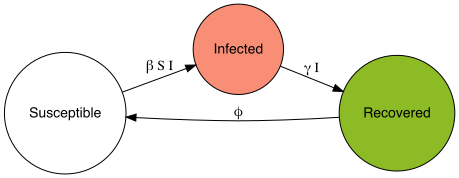
\includegraphics[width=\textwidth]{figure/sirs_model.png}
\caption[Susceptible-Infected-Recovered-Susceptible (SIRS) model]{\textbf{A SIR model with waning immunity (SIRS).} The waning parameter represents the flow of individuals who have lost their natural immunity from the recovered back to the susceptible compartment.}
\label{fig:sirs}
\end{figure}

\subsection{\texorpdfstring{Force of Infection and the Basic Reproduction Number (\(R_0\))}{Force of Infection and the Basic Reproduction Number (R\_0)}}\label{FOI-and-R0}

In equation \ref{eq:sir ode}, for \(\frac{dS}{dt}\), the term \(\beta \frac{I}{N} S\) represents the rate at which susceptible are becoming infected. Here, \(\lambda = \beta \frac{I}{N}\) is the \emph{force of infection}, which means that each susceptible individual has a probability \(\lambda\) of becoming infected per unit time. The force of infection is defined as as the per capita rate at which susceptible individuals contract the disease. Essentially, it quantifies the risk that a susceptible individual faces of becoming infected at a given time, depending on the current prevalence and contagiousness of the disease in the population. The force of infection is directly proportional to the number of infectious individuals in the population.

An infectious individual contacts \(\beta\) individuals per unit time, and the proportion of susceptibles in the population is \(\frac{S}{N}\). Therefore, the effective contacts that can result in a new infection are \(\beta \frac{S}{N}\). An infectious individual remains infectious for \(\frac{1}{\gamma}\) units of time, on average (since \(\gamma\) is the rate at which individuals recover and cease being infectious). The \emph{basic reproduction number} \(R_0\) can be calculated as the product of the infection rate per contact, the number of contacts per unit time, and the duration of infectiousness:
\[
   R_0 = \beta \frac{S}{N} \frac{1}{\gamma} = \frac{\beta}{\gamma}.
   \]
Therefore \(R_0\) is the average number of secondary cases of disease caused by a single infected individual overtheir infectious period. {[}21{]} discusses the subtleties in defining and estimating the reproductive number.

If \(R_0 > 1\), each infectious individual, on average, infects more than one other person, leading to the potential for an epidemic. Conversely, if \(R_0 < 1\), the disease will likely die out in the population over time. Understanding \(R_0\) helps in predicting disease behavior and controlling outbreaks. For instance if we can reduce \(\beta\) (e.g., through vaccination, social distancing, or wearing masks), or increase \(\gamma\) (e.g., through faster diagnosis and treatment), \(R_0\) can be brought below 1, aiming to control the spread of the disease.

\chapter{Materials and methods}\label{Materials-and-methods}

This chapter covers the technical details of using semi-mechanistic models. There are two main aspects. The first aspect explains how to construct linear smoothers using the \texttt{mgcv} package. The second aspect describes how to implement these linear smoothers within a compartmental modeling framework using \texttt{macpan2}. If your goal is to implement your own model in \texttt{macpan2} using the smoothing parameter estimation methodology to infer a latent variable by fitting the model to data, this chapter provides the general methodology to do so. It also addresses some of the unique technical issues we encountered and their solutions.

\section{Software}\label{Software}

\emph{McMaster Pandemic 2} (\texttt{macpan2}) is an \texttt{R} modeling package designed as a compartmental modeling tool that is agnostic about its underlying computational framework, though it currently uses Template Model Builder (\texttt{TMB}). It allows users to write complex, bespoke compartmental models in a user-friendly way.

\emph{Template Model Builder} (\texttt{TMB}) is an R package specifically designed to fit latent variable models efficiently to data. With \texttt{macpan2}, users can write the negative log-likelihood of their objective function with respect to the parameters to be fit to the data in R code. \texttt{macpan2} then converts this objective function to \texttt{C++} code. It implements maximum likelihood estimation and uncertainty calculations by maximizing the Laplace approximation of the marginal likelihood.

The use of the Laplace approximation to estimate model parameters and their uncertainties (using the delta method) involves the computation of first and second-order derivatives, respectively. Nonlinear optimization algorithms that use quasi-Newton methods (such as \texttt{nlminb} or BFGS) leverage differences of gradients to iteratively approximate the Hessian matrix. Accurate estimates of the gradient function are essential for the quasi-Newton algorithm to obtain efficient parameter updates. Inaccuracies in the gradient can lead to suboptimal parameter updates, slow convergence, or convergence to non-optimal points. \texttt{TMB} harnesses the capabilities of \emph{automatic differentiation} (AD), a computational technique for accurately calculating derivatives of functions. Unlike numerical or symbolic differentiation, AD operates by exploiting the fact that all computationally implemented functions decompose into a finite sequence of elementary arithmetic operations and functions {[}22{]}. Using the chain rule, AD breaks down these complex functions into simpler operations, computing derivatives in a sequence that parallels the function's evaluation. This method enables the precise calculation of derivatives up to machine precision. AD helps efficiently implement the Laplace Approximation because finite differences is a crude and slow method. For its implementation of AD, \texttt{TMB} utilizes the \texttt{C++} libraries \texttt{CppAD} for automatic differentiation and \texttt{Eigen} for handling both sparse and dense matrix computations.

In \texttt{macpan2}, specifying that the optimizer includes uncertainty estimates for parameters is straight forward. This functionality enables the computation of Wald confidence intervals with specified uncertainty levels using the delta method. This requires the computation of the Hessian matrix, which AD makes computationally efficient. Confidence intervals, as discussed in chapter \ref{Results}, are computed using this method.

For further reading on \texttt{TMB}, refer to {[}23{]}. For more information on the Laplace Approximation, see {[}24{]}. Refer to section \ref{Initial-conditions-and-parameters} for details on deriving the objective function for the semi-mechanistic model and its implementation in \texttt{macpan2}.

\section{Time varying transmission rate}\label{Time-varying-transmission-rate}

We specify the \emph{time-varying transmission rate} \(\beta\) in our model using a linear smoother defined as

\begin{equation}
\beta = \text{exp}(b_0 + \mathbf{X}b),
\label{eq:linear smoother}
\end{equation}

where \(b_0\) is the intercept, \(\mathbf{X}\) is the basis matrix of dimensions \(n \times (k-1)\), and \(b\) is a vector of basis coefficients of length \(k-1\). The basis matrix \(\mathbf{X}\) is constructed using the \texttt{smoothCon} function from the \texttt{mgcv} package in R. The structure of \(\mathbf{X}\) depends on the selected type of smoother, as indicated by the \texttt{bs} arguement, and the number of knots \(k\).

The \texttt{R} package \emph{Mixed GAM Computation Vehicle with Automatic Smoothness Estimation} (\texttt{mgcv}), developed by Simon Wood, implements a variety of smoothers that can be used for penalized generalized additive models. In our approach, we utilize \texttt{smoothCon} to create the model matrix \(\mathbf{X}\) and its corresponding penalty matrix \(\mathbf{P}\) for \(\beta\). This function facilitates the capture of the nonlinear relationships of the latent variable \(\beta\) from the data by constructing a univariate Gaussian regression smoother. While typically used internally by \texttt{mgcv} in calls to the \texttt{gam} function for fitting generalized additive models, \texttt{smoothCon} serves as a critical low-level function for constructing smooth terms in our model.

This function is configured via the \texttt{bs} argument to select the type of smoother and the \texttt{k} argument to determine the number of basis functions, which we refer to as \texttt{num\_variables}. The number of observations in the data is represented by \texttt{n}. The initial step involves constructing a simple data frame \texttt{dd\ =\ seq(from\ =\ 0,\ to\ =\ n,\ by\ =\ 1)}, which discretizes our time variable into intervals that map directly onto the domain over which the smoother operates.

The command to execute this configuration in R is as follows:

\begin{Shaded}
\begin{Highlighting}[]
\NormalTok{    s }\OtherTok{\textless{}{-}} \FunctionTok{smoothCon}\NormalTok{(}\AttributeTok{object =} \FunctionTok{s}\NormalTok{(time, }\AttributeTok{bs =}\NormalTok{ smooth, }\AttributeTok{k =}\NormalTok{ num\_variables),}
                   \AttributeTok{absorb.cons =} \ConstantTok{TRUE}\NormalTok{, }\AttributeTok{data =}\NormalTok{ dd, }\AttributeTok{knots =} \ConstantTok{NULL}\NormalTok{)}
\end{Highlighting}
\end{Shaded}

This function call yields two components for the model: the basis matrix \(\mathbf{X}\) and the penalty matrix \(\mathbf{P}\).

For instance, specifying \texttt{bs\ =\ cr} configures the basis and penalty matrices for a cubic regression spline, which is detailed further in the subsection \ref{Cubic-regression-splines}. Alternatively, when using \texttt{bs\ =\ gp} for a Gaussian process regression smoother, it becomes necessary to define the kernel type within the additional arguments (\texttt{...}). Guidelines on kernel specification and available smooths can be found in Simon Wood's \texttt{mgcv} package documentation {[}25{]}.

Details on the range of smoothers implemented in our models and their respective kernel choices are discussed in the chapter \ref{Results}.

The argument \texttt{absorb.cons\ =\ TRUE} absorbs the identifiability constraints into the basis matrix, instead of treating them as external conditions or adding them through additional penalty terms. The default \emph{identifiability constraint} in \texttt{mgcv} ensures the smooth sums to zero over the observed values of \(x_j\), i.e,

\[
1^T\mathbf{X\beta} = 0.
\]

This implies \(1^T\mathbf{X} = 0\).

\texttt{mgcv} implements this constraint by constructing the following QR decomposition.

Let

\[ 
\mathbf{C}^T = \mathbf{U} \begin{bmatrix} \mathbf{P} & 0 \end{bmatrix}, 
\]
where \(\mathbf{U}\) is a \(p \times p\) orthogonal matrix and \(\mathbf{P}\) is an \(m \times m\) upper triangular matrix. The zero matrix appended to \(\mathbf{P}\) is \(m \times (p-m)\) to match the dimensions of \(\mathbf{U}\). Now, \(\mathbf{U}\) is partitioned as \(\mathbf{U} \equiv (\mathbf{D} : \mathbf{Z})\), where \(\mathbf{D}\) is a \(p \times m\) matrix and \(\mathbf{Z}\) is a \(p \times (p-m)\) matrix.

Given that \(\beta = \mathbf{Z}\beta_z\) and \(\beta_z\) is a \((p-m)\)-dimensional vector, we compute:
\[
   \mathbf{C}\beta = \begin{bmatrix} \mathbf{P}^T \\ 0 \end{bmatrix} \begin{bmatrix} \mathbf{D}^T \\ \mathbf{Z}^T \end{bmatrix} \mathbf{Z}\beta_z = \begin{bmatrix} \mathbf{P}^T\mathbf{D}^T \\ 0 \end{bmatrix} \mathbf{Z}\beta_z = \begin{bmatrix} \mathbf{P}^T \\ 0 \end{bmatrix} \beta_z = 0,
   \]
where we used the fact that \(\mathbf{D}^T\mathbf{Z} = 0\), and \(\mathbf{Z}^T\mathbf{Z} = \mathbf{I}_{p-m}\) because \(\mathbf{U}\) is orthogonal, hence \(\mathbf{U}^T\mathbf{U} = \mathbf{I}_p\).

To minimize equation \ref{eq:penalizedregression} such that \(1^T\mathbf{X\beta} = 0\),
find the \(k \times (k-1)\) matrix \(Z\) and reparameterize the basis matrix to \(\mathbf{XZ}\) and the penalty matrix to \(\mathbf{Z^TPZ}\).

While zero-centering \(\mathbf{X}\) is a computationally more expensive method to address identifiability issues, it is still valuable to explain because it provides a clearer understanding of how the spline components and intercept interact in the model. By default, the basis matrix \(\mathbf{X}\) produced by \texttt{mgcv::smoothCon} doesn't include an intercept. Zero-centering the spline basis functions ensures that the spline components represent deviations or variations around a central tendency, rather than absolute values. This allows the intercept, \(b_0\), in the model to uniquely capture the central tendency of the response variable. Consequently, the intercept and the spline coefficients are identifiable as distinct contributors to the model: the intercept as the average response and the spline coefficients as the adjustments from this average. Each spline coefficient can be interpreted as the effect of that basis function relative to the central tendency captured by the intercept.

Zero-centering is implemented by subtracting the column mean from each column of \(\mathbf{X}\), which effectively reduces the rank of \(\mathbf{X}\) by one. This process removes one degree of freedom, corresponding to the zero eigenvalue, from the basis matrix. To resolve this, we exclude the row and column associated with the zero eigenvalue from \(\mathbf{X}\), and we also remove the corresponding element from the vector of coefficients, \(\beta\). This adjustment ensures that the remaining components of \(\mathbf{X}\) and \(\beta\) are identifiable.

\(\mathbf{X}\) and \(b\) now have one fewer dimension than the number of knots due to the null space of the penalty matrix. The penalty matrix's null space dimension of one means the function can vary linearly without penalty. As \(\lambda\) increases, the model reverts to a linear trend because this minimizes penalized complexity under high penalty values.

There are difficulties encountered when working with the penalty matrix that has been transformed into the constraint space of the sum to zero constraint. Computing the eigendecomposition of the penalty matrix, returned by \texttt{mgcv::smoothCon}, one of the eigenvalues is essentially zero, in terms of numerical precision, being on the order of \(\leq 10^{-10}\). This implies that the penalty matrix is singular. It is not possible to take the logarithmic determinant of a singular matrix when taking numerical precision limitations into account. Computing the log determinant is part of the objective equation (\ref{eq:obj eqn}). To overcome this we can take the regularized determinant by adding a small value (\(\approx 10^{-5})\)) to the diagonal of the penalty matrix. Another option (which we did not implement) is to take the singular value decomposition \(\mathbf{P} = \mathbf{U}\mathbf{\Sigma} \mathbf{V}^T\) and use the fact that \(\text{logdet}\mathbf{P}= \sum_i \text{log}\Sigma_{ii}\).

We scaled \(\mathbf{X}\) to make it compatible across bases, with a choice of the standard deviation used to simulate the starting values for \(\beta\). Each column of the basis matrix \(\mathbf{X}\) is normalized by dividing it by its Euclidean norm, resulting in each column having a unit norm. Then \(\mathbf{X}\beta\) is on the range of about of plus or minus \(\text{log}(2)\) (i.e \(\mathbf{X}\beta \pm 1)\), since

\[
\beta \sim \mathcal{N}(0, b_{sd}).
\]

When the sum-to-zero constraints are absorbed into the basis matrix, this also sets the penalty matrix for the Gaussian process to have the last row and column equal to zero, effectively absorbing the null space constraints into the penalty matrix. This makes \(\mathbf{P}\) singular. If we remove the final row and column of \(\mathbf{P}\), then we get a non-singular matrix.

\section{Time-varying effective reproduction number}\label{Time-varying-effective-reproduction-number}

The effective reproductive number

\[
R_t = R_0 \times \frac{S(t)}{N} = \frac{\beta}{\gamma} \times \frac{S(t)}{N},
\]
dynamically reflects the average number of secondary infections that an infectious individual can cause at a specific time \(t\) in a population where not all members are susceptible. This equation implies that \(R_t\) will decrease over time as \(S(t)\) decreases. It also implies that \(R_t\) can be effectively reduced by decreasing the contact rate \(\beta(t)\) through interventions. Unlike \(R_0\), which assumes that the entire population is susceptible, \(R_t\) adjusts for changes in susceptibility due to factors such as immunity from previous infections or vaccinations.

As the epidemic progresses, the proportion of susceptible individuals decreases either through infection---which can lead to immunity or death---or through vaccination. This reduction in the susceptible population is quantified by \(S(t)/N\), where \(S(t)\) represents the number of susceptible individuals at time \(t\), and \(N\) is the total population.

Instead of treating \(\beta\) as a constant, it is estimated as a smooth function. This allows \(\beta\), the time-varying transmission parameter, to adapt and change over time, resulting in the sequence \(\{\beta(t_i)\}_{i=1}^n\). Meanwhile, the recovery rate \(\gamma\) remains fixed at its initial value. Consequently, this framework enables the calculation of the \emph{time varying effective reproductive number}

\[
     R_t = \frac{\beta(t)}{\gamma} \times \frac{S(t)}{N},
\]
based on the dynamically adjusting \(\beta\).

Note that in some definitions of the time varying effective reproduction number, both \(\gamma\) and \(\beta\) are estimated as time-varying parameters. However, in this context, \(\gamma\) is treated as a constant. In Chapter \ref{Results}, the starting value of \(\gamma\) for each disease is derived from existing literature. Meanwhile, in the simulation study, \(\gamma\) is assigned a reasonable fixed value.

In section \ref{Time-varying-transmission-rate} we described how to estimate a time varying transmission parameter to compute estimates for the force of infection. This estimate is then used to compute the time varying effective reproduction number.

\section{Inititial conditions and parameters}\label{Initial-conditions-and-parameters}

The simulation study employs the SIRS model, while the examples uses the SIR model. The simulation study initializes the starting values of \(S\), \(I\), and \(R\) to the following endemic equilibrium states:

\[
\begin{aligned}
S &= \frac{\gamma N}{\beta}, \\
I &= \frac{\phi N (\beta - \gamma)}{\beta(\phi + \gamma)}, \\
R &= \frac{\gamma N (\beta - \gamma)}{\beta (\phi + \gamma)}.
\end{aligned}
\]

By initializing the compartment values deterministically as functions of the total population \(N\), the transmission rate \(\beta\), the recovery rate \(\gamma\), and the waning rate \(\phi\), we can start the simulation close to the endemic equilibrium. This approach stabilizes the influence of the starting parameters, particularly \(\beta\), on the model dynamics. Consequently, the system begins in a balanced state, reducing the transient effects that might otherwise occur due to arbitrary initial conditions. This transformation was not necessary for the real-world data examples.

For these examples, the state vectors are initialized as follows:

\[
\begin{aligned}
S &= N - I_0, \\
I &= I_0, \\
R &= 0.
\end{aligned}
\]

The \emph{initial number of infected individuals}, \(I_0\), at time \(t=0\) is modeled as a fixed parameter. To account for uncertainty about \(I_0\), we employ a log-normal prior distribution. We use a similar approach for the recovery rate \(\gamma\), also modeled with a log-normal prior to ensure positivity and reflect our uncertainty regarding its value. Specifically, we set the mean of the priors to the logarithmic values of \(I_0\) and \(\gamma\), and the standard deviation for each parameter is set to a small reasonable value \(\sigma = 0.1\) to instill a sharp prior.

The smoothing coefficients vector \(b = (b_1, \ldots, b_{k-2})\) is initialized using \(k-1\) random draws from a standard normal distribution.

The intercept \(b_0\) of the linear smoother (\ref{eq:linear smoother}), for the time varying transmission, is estimated in the model. It starting value is set to the logarithm of the starting value of \(\beta\) at time \(t= 0\).

We can compute the likelihood of the basis coefficients by making the assumption that
the spline basis coefficients \(\beta\) follow a multivariate Gaussian distribution, i.e., \(\beta \sim \mathcal{N}(\mathbf{0}, \mathbf{\Sigma})\). The log likelihood function for \(\beta\) is then

\[
L(\beta) = -\frac{k}{2} \log(2\pi) -\frac{1}{2} \log(\text{det}(\mathbf{\Sigma})) -\frac{1}{2} (\mathbf{x}-\mu)^T \mathbf{\Sigma}^{-1} (\mathbf{x}-\mu).
\]

Now let \(\beta = \mathbf{x}- \mu\) and \(\Sigma^{-1}= a\mathbf{S}\), where \(a = \frac{1}{\sigma^2}\), \(\sigma^2 \in \mathbb{R}\) and \(\mathbf{S}\) is the penalty matrix. This implies \(\mathbf{\Sigma} = a^{-1}\mathbf{S}^{-1}= \sigma^2\mathbf{S}^{-1}\).

Then,

\begin{equation}
L(\beta) = -\frac{k}{2} \log(2\pi) - \frac{1}{2} \log(\sigma^2) -  \log(\text{det}(\mathbf{S})) + \frac{1}{2\sigma^2} \beta^T \mathbf{S} \beta.
\label{eq:obj eqn}
\end{equation}

The term \(\sigma^2\) represents a variance component that scales the penalty matrix \(\mathbf{S}\). It acts as a global variance parameter that moderates the extent to which the penalty is applied. By scaling \(\mathbf{S}\) with \(\sigma^2\), you effectively adjust the strength of the regularization relative to the variance of the data. Consequently, \(\lambda = \frac{1}{2\sigma^2}\) functions as a regularization parameter, controlling the ``wiggliness'' of the fit by influencing the variance of the distribution of the smoothing coefficients. This setup can be viewed as placing a prior distribution on \(\beta\), with \(\mathbf{S}\) acting as the precision matrix of the prior. This approach is analogous to the Bayesian perspective of smoothing, as discussed in equation \ref{eq:penalty prior}. Here, \(\sigma^2\) scales the precision matrix of the prior, influencing how strongly the prior beliefs (e.g., smoothness) affect the posterior estimates.

Therefore \(L(\beta)\) is the derived form of the penalty functional \(J(f)\) in equation \ref{eq: general penalized spline} when the smoothing coefficients are assumed to be Gaussian.

Considering the data model \(Y_i = f(x_i) + \epsilon_i\), where \(i = 1, \dots, n\) and \(\epsilon_i \sim \text{N}(0, \sigma^2)\), the likelihood functional \(L(f|\text{data})\) in equation \ref{eq: general penalized spline} simplifies to a least squares functional. This is proportional to \(\sum_{i=1}^n (Y_i - f(x_i))^2\), aligning with the Gaussian likelihood. Therefore, the likelihood can be expressed using a Gaussian density function evaluated at the vector of observed values \(\mathbf{Y}\), with mean \(f(\mathbf{x})\) and variance \(\sigma^2_Y\).

Thus, to fit the combined objective function \(L(f|\text{data}) + J(f)\), we estimate both the smoothing parameter \(\lambda\) and the variance \(\sigma^2_Y\).

The number of basis functions or knots to use in the model is not algorithmically optimized. The basis dimension \(k\) was chosen to be just large enough that the plotted fits appeared to converge to a stable fit. In {[}9{]}, Simon Wood outlines the methodology to compute a quantitative measure of whether a particular choice of basis dimension is appropriate. However, in our case, the smoothing parameter does most of the work in avoiding overfitting.

\section{Model formulation}\label{Model-formulation}

Recall the following assumptions in the model:

\[
\begin{aligned}
I_0 &\sim \text{Lognormal}(\mu_{I_0}, \sigma^2_{I_0}) \\
\gamma &\sim \text{Lognormal}(\mu_{\gamma}, \sigma^2_{\gamma}) \\
Y &\sim \mathcal{N}(f(x), \sigma^2_Y) \\
\beta &\sim \mathcal{N}(0, \frac{\mathbf{S}^{-1}}{\sigma^2}),
\end{aligned}
\]
where \(f(x)\) is the fitted values (incidence). Note that
we are not estimating the observed values \(Y\) but estimating the variance \(\sigma^2_Y\) corresponding to its likelihood equation. In this way the fitted values \(f(x)\) behave as a sort of Gaussian process.

The model assumptions and starting conditions are specified and passed to a simulator object in \texttt{macpan2}. \texttt{TMB} simulates the trajectory using the Euler method.

At \(t= 0\) the smoothing basis \(\mathbf{X}\), the vector of smoothing coefficients \(b\) and its intercept \(b_0\) are used to construct the transmission rate \(\beta\), a vector equal to the number of observations, of size \(n\). At each time step, \(1 \leq t \leq n\), \(\beta\) is used to compute the number of new infections (\texttt{incidence}), which in turn is used to compute the total number of infected (\texttt{I}) and susceptible (\texttt{S}) at that time point. Additionally, \(\beta\) is used to compute the instantaneous effective reproduction number \(R_t\).

After simulating the trajectory, the negative log likelihood is minimized subject to finding the optimal values of the starting values of the initial number of infected \(I_0\), the recovery rate \(\gamma\), the variance \(\sigma^2_Y\) of likelihood of the observed data and the regularization/smoothing parameter \(\sigma^2\). Note that the priors on the recovery rate and the initial number of infected are not `fully Bayesian' in the sense that there are not priors placed on the mean and variance of the prior distribution, i.e no there are no hyper-priors. Parameter estimates for the intercept \(b_0\) of the linear smoother are also obtained.

For each iteration, the simulated trajectory is matched to the observed values and the likelihood is calculated using the Laplace approximation. New parameter estimates are updated using Quasi-Newton methods via \texttt{nlminb}. This process is then iterated until the parameter estimates converge.

Here is an example of what the simulator object for an SIR model in \texttt{macpan2} looks like using the above formulation:

\begin{Shaded}
\begin{Highlighting}[]
\SpecialCharTok{{-}{-}{-}{-}{-}{-}{-}{-}{-}{-}{-}{-}{-}{-}{-}{-}{-}{-}{-}{-}{-}}
\NormalTok{Before the simulation }\FunctionTok{loop}\NormalTok{ (}\AttributeTok{t =} \DecValTok{0}\NormalTok{)}\SpecialCharTok{:}
\SpecialCharTok{{-}{-}{-}{-}{-}{-}{-}{-}{-}{-}{-}{-}{-}{-}{-}{-}{-}{-}{-}{-}{-}}
\DecValTok{1}\SpecialCharTok{:}\NormalTok{ I\_0 }\SpecialCharTok{\textasciitilde{}} \FunctionTok{exp}\NormalTok{(log\_I\_0)}
\DecValTok{2}\SpecialCharTok{:}\NormalTok{ gamma }\SpecialCharTok{\textasciitilde{}} \FunctionTok{exp}\NormalTok{(log\_gamma)}
\DecValTok{3}\SpecialCharTok{:}\NormalTok{ lambda }\SpecialCharTok{\textasciitilde{}} \FunctionTok{exp}\NormalTok{(log\_lambda)}
\DecValTok{4}\SpecialCharTok{:}\NormalTok{ I\_sd }\SpecialCharTok{\textasciitilde{}} \FunctionTok{exp}\NormalTok{(log\_I\_sd)}
\DecValTok{5}\SpecialCharTok{:}\NormalTok{ S }\SpecialCharTok{\textasciitilde{}}\NormalTok{ N }\SpecialCharTok{{-}}\NormalTok{ I\_0}
\DecValTok{6}\SpecialCharTok{:}\NormalTok{ R }\SpecialCharTok{\textasciitilde{}} \DecValTok{0}
\DecValTok{7}\SpecialCharTok{:}\NormalTok{ I }\SpecialCharTok{\textasciitilde{}}\NormalTok{ I\_0}
\DecValTok{8}\SpecialCharTok{:}\NormalTok{ S }\SpecialCharTok{\textasciitilde{}}\NormalTok{ N }\SpecialCharTok{{-}}\NormalTok{ I }\SpecialCharTok{{-}}\NormalTok{ R}
\DecValTok{9}\SpecialCharTok{:}\NormalTok{ eta }\SpecialCharTok{\textasciitilde{}}\NormalTok{ b\_0 }\SpecialCharTok{+}\NormalTok{ (X }\SpecialCharTok{\%*\%}\NormalTok{ b)}

\SpecialCharTok{{-}{-}{-}{-}{-}{-}{-}{-}{-}{-}{-}{-}{-}{-}{-}{-}{-}{-}{-}{-}{-}}
\NormalTok{At every iteration of the simulation }\FunctionTok{loop}\NormalTok{ (}\AttributeTok{t =} \DecValTok{1}\NormalTok{ to n)}\SpecialCharTok{:}
\SpecialCharTok{{-}{-}{-}{-}{-}{-}{-}{-}{-}{-}{-}{-}{-}{-}{-}{-}{-}{-}{-}{-}{-}}
\DecValTok{1}\SpecialCharTok{:}\NormalTok{ beta }\SpecialCharTok{\textasciitilde{}} \FunctionTok{exp}\NormalTok{(eta[}\FunctionTok{time\_step}\NormalTok{(}\DecValTok{1}\NormalTok{)])}
\DecValTok{2}\SpecialCharTok{:}\NormalTok{ R\_t }\SpecialCharTok{\textasciitilde{}}\NormalTok{ (}\FunctionTok{log}\NormalTok{(beta) }\SpecialCharTok{{-}} \FunctionTok{log}\NormalTok{(gamma) }\SpecialCharTok{+} \FunctionTok{log}\NormalTok{(S) }\SpecialCharTok{{-}} \FunctionTok{log}\NormalTok{(N))}
\DecValTok{3}\SpecialCharTok{:}\NormalTok{ incidence }\SpecialCharTok{\textasciitilde{}}\NormalTok{ S }\SpecialCharTok{*}\NormalTok{ I }\SpecialCharTok{*}\NormalTok{ beta}\SpecialCharTok{/}\NormalTok{N}
\DecValTok{4}\SpecialCharTok{:}\NormalTok{ recovery }\SpecialCharTok{\textasciitilde{}}\NormalTok{ gamma }\SpecialCharTok{*}\NormalTok{ I}
\DecValTok{5}\SpecialCharTok{:}\NormalTok{ S }\SpecialCharTok{\textasciitilde{}}\NormalTok{ S }\SpecialCharTok{{-}}\NormalTok{ incidence}
\DecValTok{6}\SpecialCharTok{:}\NormalTok{ I }\SpecialCharTok{\textasciitilde{}}\NormalTok{ I }\SpecialCharTok{+}\NormalTok{ incidence }\SpecialCharTok{{-}}\NormalTok{ recovery}
\DecValTok{7}\SpecialCharTok{:}\NormalTok{ R }\SpecialCharTok{\textasciitilde{}}\NormalTok{ R }\SpecialCharTok{+}\NormalTok{ recovery}

\SpecialCharTok{{-}{-}{-}{-}{-}{-}{-}{-}{-}{-}{-}{-}{-}{-}{-}{-}{-}{-}{-}{-}{-}}
\NormalTok{After the simulation }\FunctionTok{loop}\NormalTok{ (}\AttributeTok{t =}\NormalTok{ n}\SpecialCharTok{+}\DecValTok{1}\NormalTok{)}\SpecialCharTok{:}
\SpecialCharTok{{-}{-}{-}{-}{-}{-}{-}{-}{-}{-}{-}{-}{-}{-}{-}{-}{-}{-}{-}{-}{-}}
\DecValTok{1}\SpecialCharTok{:}\NormalTok{ log\_lik }\SpecialCharTok{\textasciitilde{}} \SpecialCharTok{{-}}\FunctionTok{sum}\NormalTok{(}\FunctionTok{dnorm}\NormalTok{(incidence\_obs, incidence\_fitted, incidence\_sd)) }\SpecialCharTok{{-}}
              \FunctionTok{dnorm}\NormalTok{(log\_gamma, mean\_log\_gamma, sd\_log\_gamma) }\SpecialCharTok{{-}} 
              \FunctionTok{dnorm}\NormalTok{(log\_I\_0, mean\_log\_I\_0, sd\_log\_I\_0) }\SpecialCharTok{+}
              \FunctionTok{log}\NormalTok{(}\FunctionTok{det}\NormalTok{(P)) }\SpecialCharTok{{-}}
              \FunctionTok{log}\NormalTok{(sigma}\SpecialCharTok{\^{}}\DecValTok{2}\NormalTok{) }\SpecialCharTok{+} 
\NormalTok{              ((}\FunctionTok{t}\NormalTok{(b) }\SpecialCharTok{\%*\%}\NormalTok{ P }\SpecialCharTok{\%*\%}\NormalTok{ b) }\SpecialCharTok{/}\NormalTok{ sigma}\SpecialCharTok{\^{}}\DecValTok{2}\NormalTok{)}
\end{Highlighting}
\end{Shaded}

Sometimes it is useful to simulate the trajectory for \(n\) time steps and then calibrate the model over a smaller time series by aggregating the data into \(\frac{n}{k}\) time steps by averaging the trajectory and data over a period of \(k\) steps. For example, in the case of the Ireland Covid-19 dataset (\ref{Ireland}), the reported incidence was inconsistent on a daily scale. By averaging the observations over a weekly scale, the variance is reduced as the averaging process diminishes the day-to-day fluctuations caused by sporadic reporting.

Extra care is needed to handle the uncertainty estimates of aggregated trajectory simulations. For un-aggreggated data, \texttt{macpan2}, which has \texttt{TMB} for its optimization engine, uses the Laplace Approximation to compute uncertainty estimates with the delta method. By averaging the trajectory over a time period of size \(k\), we are in effect making a transformation of a random variable. The uncertainty estimates are required to take this into account. The variance of a function \(h(\beta) = \mathbf{H} \beta\) of the random variable \(\beta\) is computed as

\[
Var(\mathbf{H} \beta) = \mathbf{H}^T Cov(\beta) \mathbf{H},
\]
where \(\mathbf{H}\) is a \(n \times n_k\) indicator matrix, where \(n_k\) is the integer ceiling of \(\frac{n}{k}\) such that \(\frac{n}{n_k} \in \mathbb{Z}\). The transformed variance is then used to compute the Wald confidence intervals as in the unaggreggated case.

\chapter{Results}\label{Results}

This chapter presents examples demonstrating the application of semi-mechanistic models in infectious disease modeling. These examples illustrate the capabilities of semi-mechanistic models. We begin with a simulated data example to showcase the effectiveness of fitting semi-mechanistic models with a single unknown function. The structure of the compartmental models is intentionally kept simple to demonstrate that estimating unknown functions using penalized smoothers is straightforward when integrated into the syntax and optimization engine of \texttt{macpan2}. The objective is to illustrate this approach so that modelers can use it without extensive knowledge of spline and nonlinear optimization literature. Following this, we provide three real-world examples: an epidemic of scarlet fever in Ontario from 1929 to 1931, the initial SARS-CoV-19 outbreak in Ireland at the start of the pandemic, and four decades of measles in London, UK.

\section{SIRS Model with Simulated Data}\label{simulation}

One challenge in epidemiological modeling is the lack of direct observation of the transmission rate within datasets containing incidence or prevalence data. Consequently, the true shape of the function used to estimate the transmission rate remains unknown. Our goal is to develop a compartmental model, formulated as a deterministic system of ordinary differential equations, incorporating a linear smoother component. If this model can accurately predict population dynamics based on the time-varying transmission rate, it should enable us to infer the transmission rate by fitting the model to the data. This approach allows us to validate the effectiveness of the smoothing parameter estimation methodology and demonstrate the applicability of these methods with models formulated as discrete systems of ordinary differential equations.

Consider the time-varying transmission rate \(\beta\) as a latent variable. `Time-varying' means that at each observation \(x_i\) in the dataset, the model---comprising a system of ordinary differential equations---contains an estimated value for the transmission rate for each \(1 \leq i \leq n\), where \(n\) is the number of observations.

\(\beta\) is constructed as the linear smoother \(b_0 + \mathbf{X}b\), where \(b_0\) is the intercept, \(\mathbf{X}\) is the model matrix associated with the particular smoother, and \(b\) is the vector of smoothing coefficients. Both \(b_0\) and \(b\) are parameters that need to be estimated. This linear smoother, which estimates \(\beta\), is a non-parametric component inside a deterministic system of differential equations, whose trajectory is determined entirely by the starting parameters. This is why the model is called semi-mechanistic or partially specified. Some components of the model contain unknown functions, while the rest of the model comprises conventional elements with only unknown scalar parameters.

To prove that semi-mechanistic models within the \texttt{macpan2} modeling framework are capable for this problem, we conduct a simulation study. For a chosen smooth, we simulate data and add Gaussian noise to the incidence. The simulated data is used to calibrate the model using various smoothers available in the \texttt{mgcv} package. In Figure \ref{fig:sim_basis}, we illustrate the shape of the basis functions for each of the univariate smoothing bases used in this methodology.

Consider a SIRS compartmental model with a fixed waning immunity parameter \(\phi\). The total number of individuals in the population is given by \(N\). The initial values of \(S\), \(I\), and \(R\) are fixed at the endemic equilibrium solutions.

We construct the data-generating model as follows. The smoother type and the number of knots \(k\) are specified using a particular \texttt{mgcv} smooth. This determines the form of \(\mathbf{X}\) and the penalty matrix \(\mathbf{P}\). The smoothing coefficients \(b\), of dimension \(k-2\), are assumed to be multivariate Gaussian. Thus, \(b\) is defined as random normal deviates at the \(k-2\) evenly spaced quantiles with a mean of 0 and a standard deviation specified as \(b_{sd}\). As the variation of this distribution increases, the true function describing the time-varying transmission rate for the data model will become more complex. An initial value for \(b_0\) is chosen as the log of the initial value of \(\beta\). The recovery rate \(\gamma\) is fixed. Initial values for the remaining parameter estimates are set to 1.

The model trajectory is simulated from these initial conditions using Euler steps. Gaussian noise (\(sd = 0.2\)) is added to the log-transformed simulated incidence vector, and then the inverse transformation is applied. This vector is used to test the efficacy of the semi-mechanistic models. The models are calibrated using \texttt{macpan2}, which uses the Laplace approximation via \texttt{TMB} to optimize the objective function and update parameter estimates using Quasi-Newton methods.

To investigate the effect of temporal aggregation on model performance, we conducted an additional study where we aggregated the simulated data on a weekly scale before fitting the model. This process involved summing the predicted incidence over each week and then fitting the model to these aggregated observations. Both the unaggregated and aggregated models use the same simulated trajectory with added noise, ensuring consistency between the two approaches. We used \(k=20\) knots to simulate the data. The aggregated data was obtained by summing the noisy unaggregated data on a weekly basis.

We performed cross-model comparison by varying the smoothing basis used to calibrate the models across the smoothing basis used to simulate the data. The variance used to generate the starting values for the smoothing coefficients \(b_{sd} = 1\) is fixed for starting values. \(\gamma = 1/7\), which represents a one-week period of an infectious individual being capable of transmitting the disease to a susceptible individual. \(\phi = \frac{1}{300}\), which means that at each time point, that proportion of the recovered individuals lose immunity. An equivalent interpretation of the waning immunity parameter is that it represents the period of immunity for an individual, which in this case represents 300 days. We have kept \(\gamma\) fixed in the simulation study, but in the real-life data examples, we have used a log-normal prior to allow flexible deviation from the initialized starting value of \(\gamma\).

In Figures \ref{fig:sim_gp}, \ref{fig:sim_tp}, \ref{fig:sim_cr}, and \ref{fig:sim_bs}, we present the results for unaggregated data simulated using the Gaussian process (GP), thin plate regression spline (TP), cubic regression spline (CR), and B-spline (BS) bases, respectively. In Figures \ref{fig:sim_agg_gp}, \ref{fig:sim_agg_tp}, \ref{fig:sim_agg_cr}, and \ref{fig:sim_agg_bs}, we present the results for aggregated data. We have chosen to omit the results of the calibration models utilizing a P-spline basis, as they show poor ability to predict incidence and infer the underlying true transmission rate when the number of knots used is less than the number used to generate the data.

For the predicted incidence, the red line represents the true value from the simulated trajectory with Gaussian noise. The blue line indicates the predicted incidence, with light and dark blue bands representing the 95\% and 50\% confidence intervals, respectively.

For the estimated transmission rate (\(\beta_t\)), the red line represents the true transmission rate function from the simulated data. The green line indicates the estimated transmission rate, with light and dark green bands representing the 95\% and 50\% confidence intervals, respectively.

For the estimated effective reproduction number \(R_t\), the black line represents the true reproduction number from the simulated data. The purple line indicates the estimated reproduction number, with light and dark purple bands representing the 95\% and 50\% confidence intervals, respectively.

The number of knots used to calibrate the models was \(k =20\) for simulated data sets, except the TP basis for both the unaggregated and aggregated data. For the GP, CR, and BS data, the value \(k =20\) was chosen as the smallest value of \(k\) to fit the predicted and estimated values without introducing overfitting. This was evaluated by visually inspecting the results of the figures below. For the TP basis, the optimization procedure for the model calibration did not converge for values of \(k \geq 10\). None of the bases were able to match the highly oscillating trajectory observed in the last 75 days of Figures \ref{fig:sim_tp} and \ref{fig:sim_agg_tp}.

In Table \ref{tab:aic-table-sim}, we present the comparison of the conditional AIC scores for all eight models. We observe that the Gaussian process (GP) model consistently has the lowest AIC score across all datasets. The AIC score, which balances model fit and complexity, suggests that the GP model provides the best trade-off between these two aspects among the models compared. A lower AIC score indicates that the GP model is relatively the best fit for the data, taking into account the effect of penalization on the number of knots used, i.e., effective degrees of freedom. Thus, the GP model is the most likely to minimize information loss when approximating the true data-generating process, compared to the other models tested.

\begin{figure}[H]
\centering
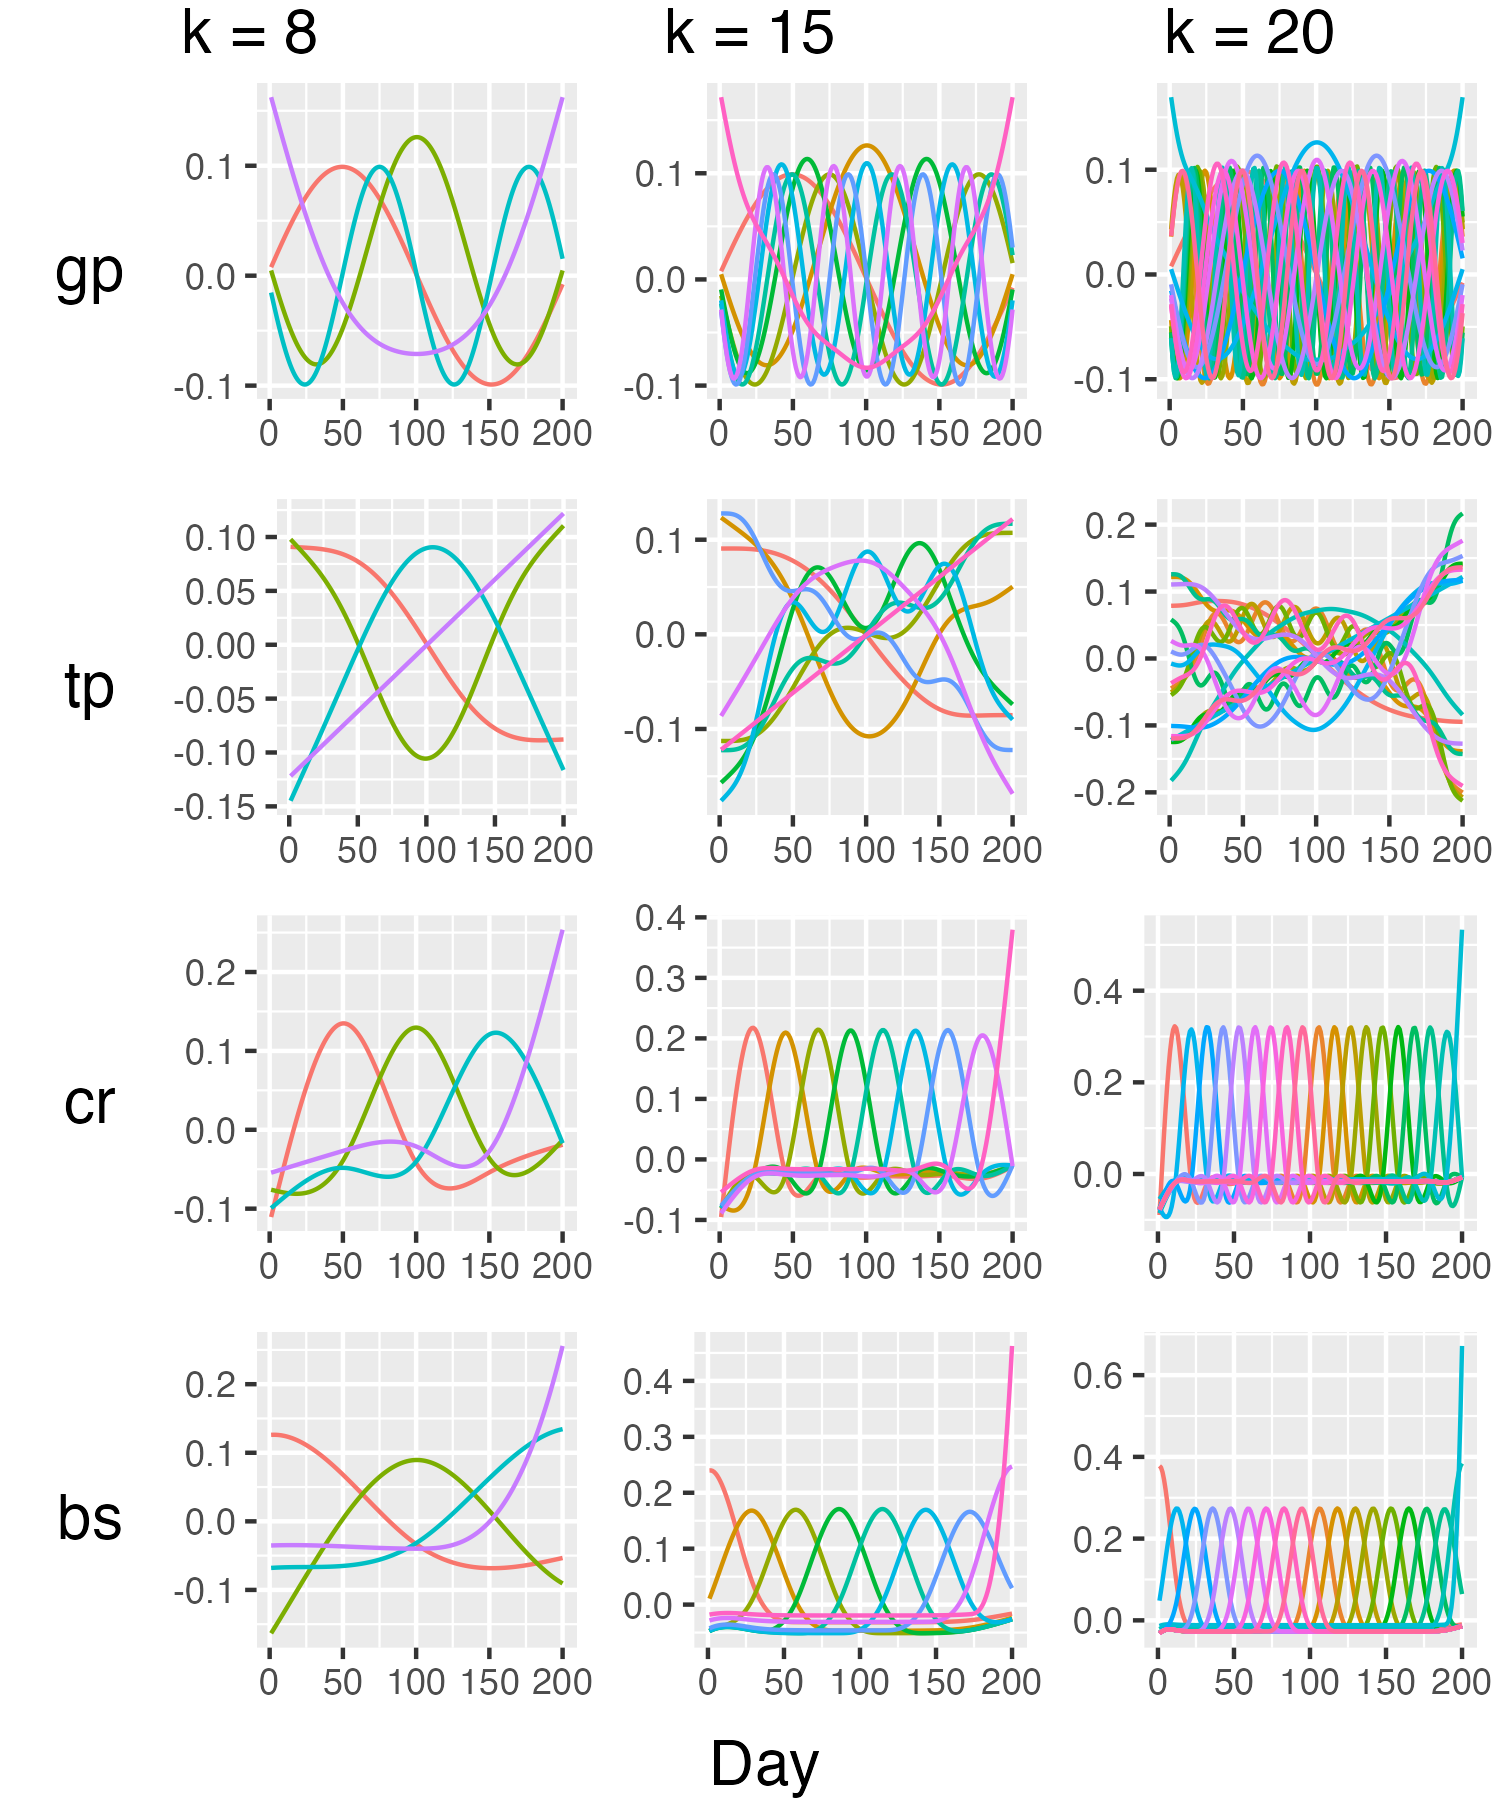
\includegraphics[width=\textwidth]{figure/Simulated/unaggregated/simulation_gp_20_k(5,10,20)_bsd1_beta1_plot_basis.png}
\caption[Basis Functions for Smoothing Basis.]{\textbf{Basis functions for calibrating smoothers}. Basis matrices are obtained via mgcv::smoothCon() with number of knots \(k=20\) and domain of \(n=200\) days. Each basis matrix is determined only by the input domain and the number of knots. Each basis function is a single column of the basis matrix. The acronyms for the smoothers are defined as follows: "gp" = Gaussian process, "tp" = thin plate regression spline, "cr" = cubic regression spline and "bs" = B-spline.}
\label{fig:sim_basis}
\end{figure}

\begin{figure}[H]
\centering
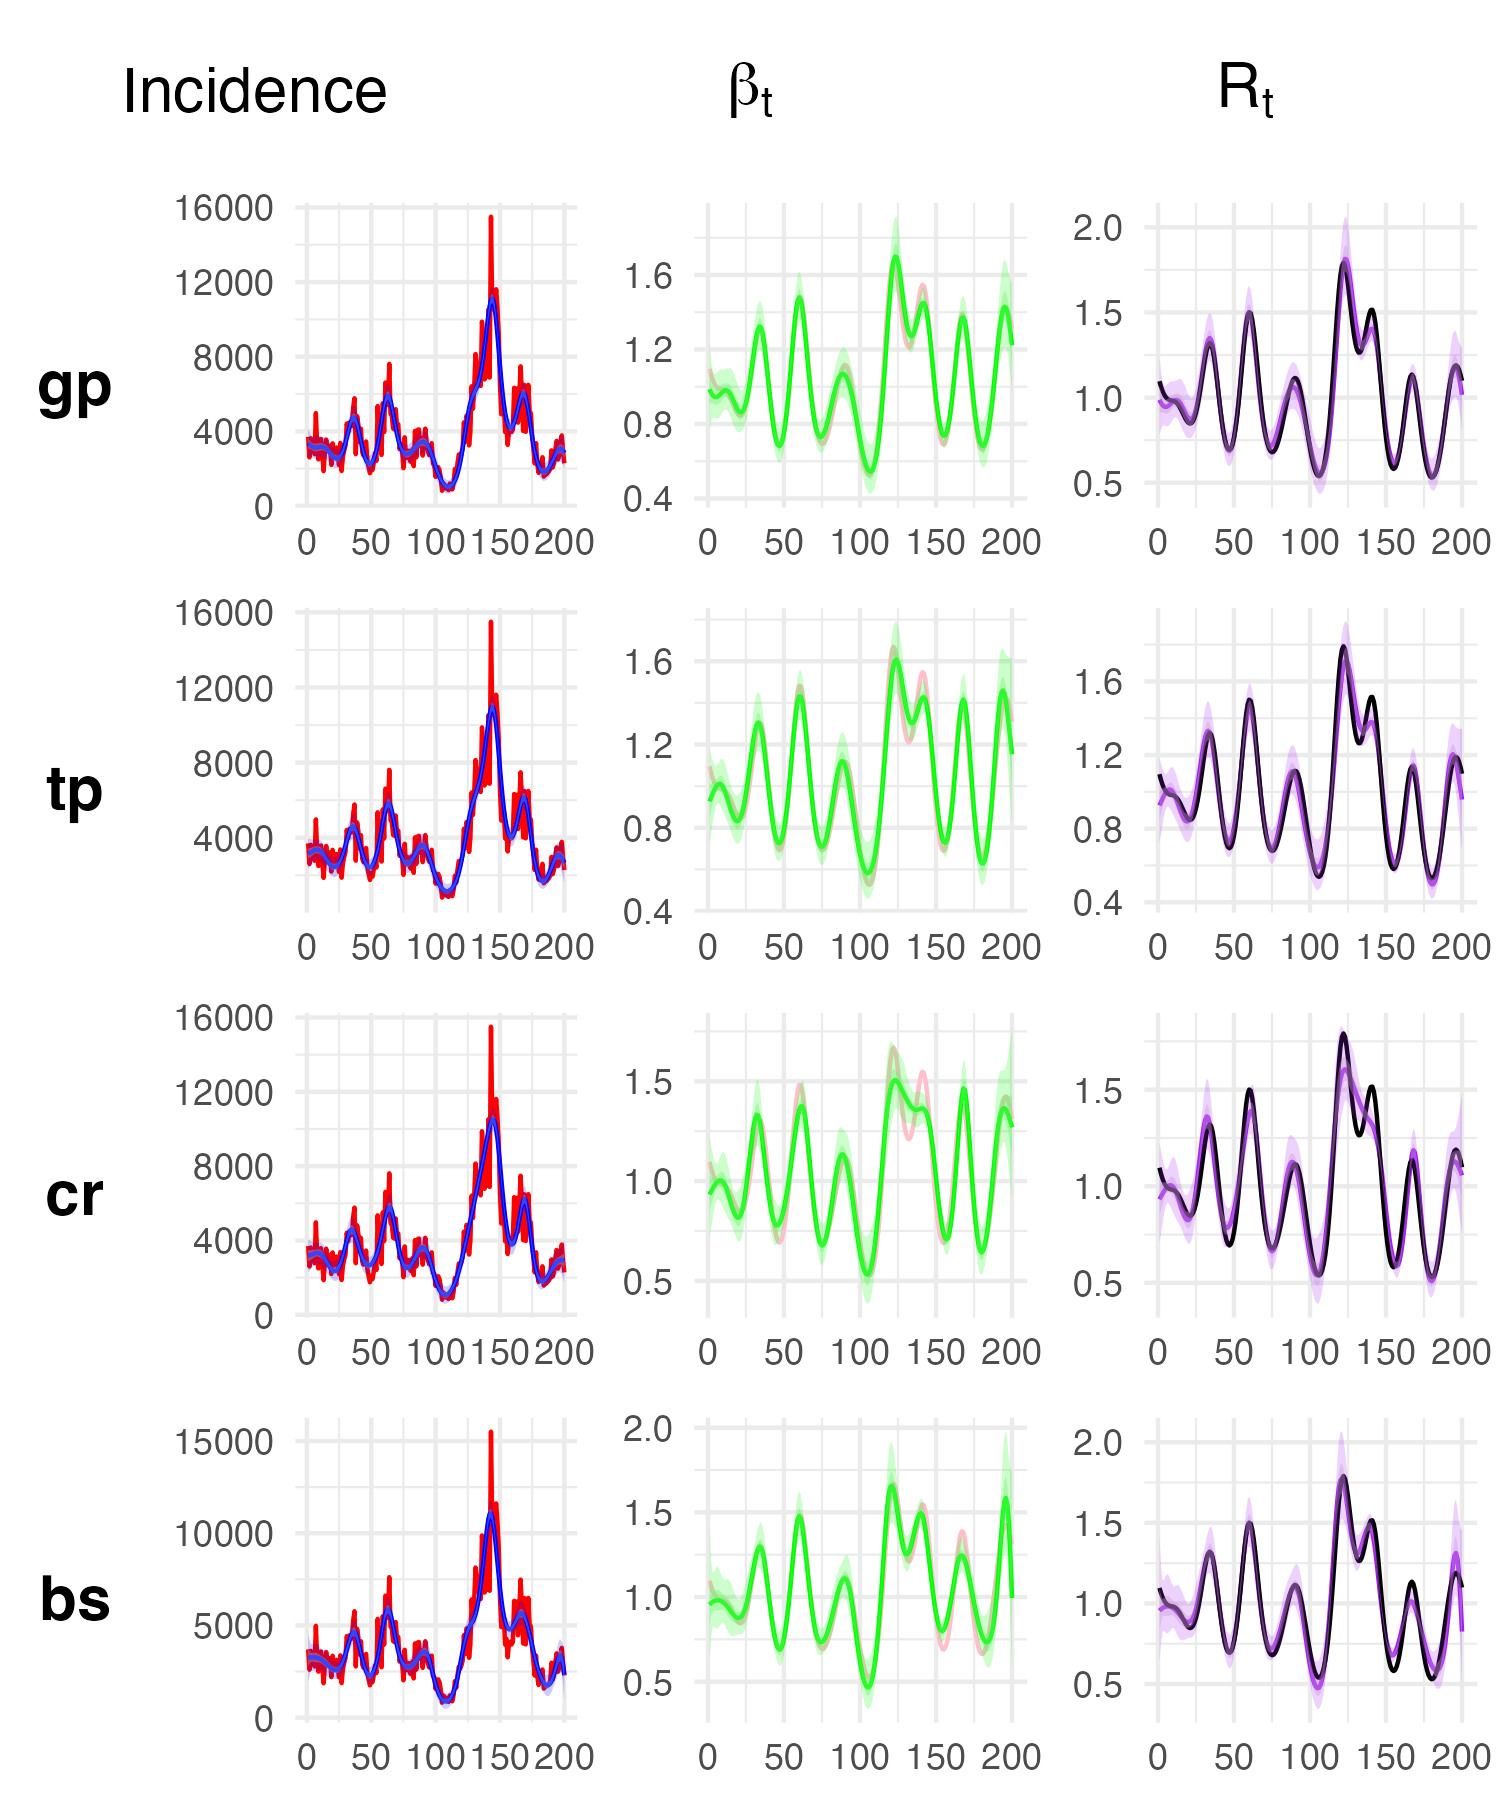
\includegraphics[width=\textwidth]{figure/Simulated/unaggregated/sim_combined_gp.png}
\caption[SIRS model with simulated data (GP).]{\textbf{SIRS Model with Simulated Data (GP).} The columns represent the predicted incidence, the estimated transmission rate and effective reproduction number. The rows correspond to the different smoothing basis used to fit the model to the data. \(k=20\) knots were used to calibrate the model.}
\label{fig:sim_gp}
\end{figure}

\begin{figure}[H]
\centering
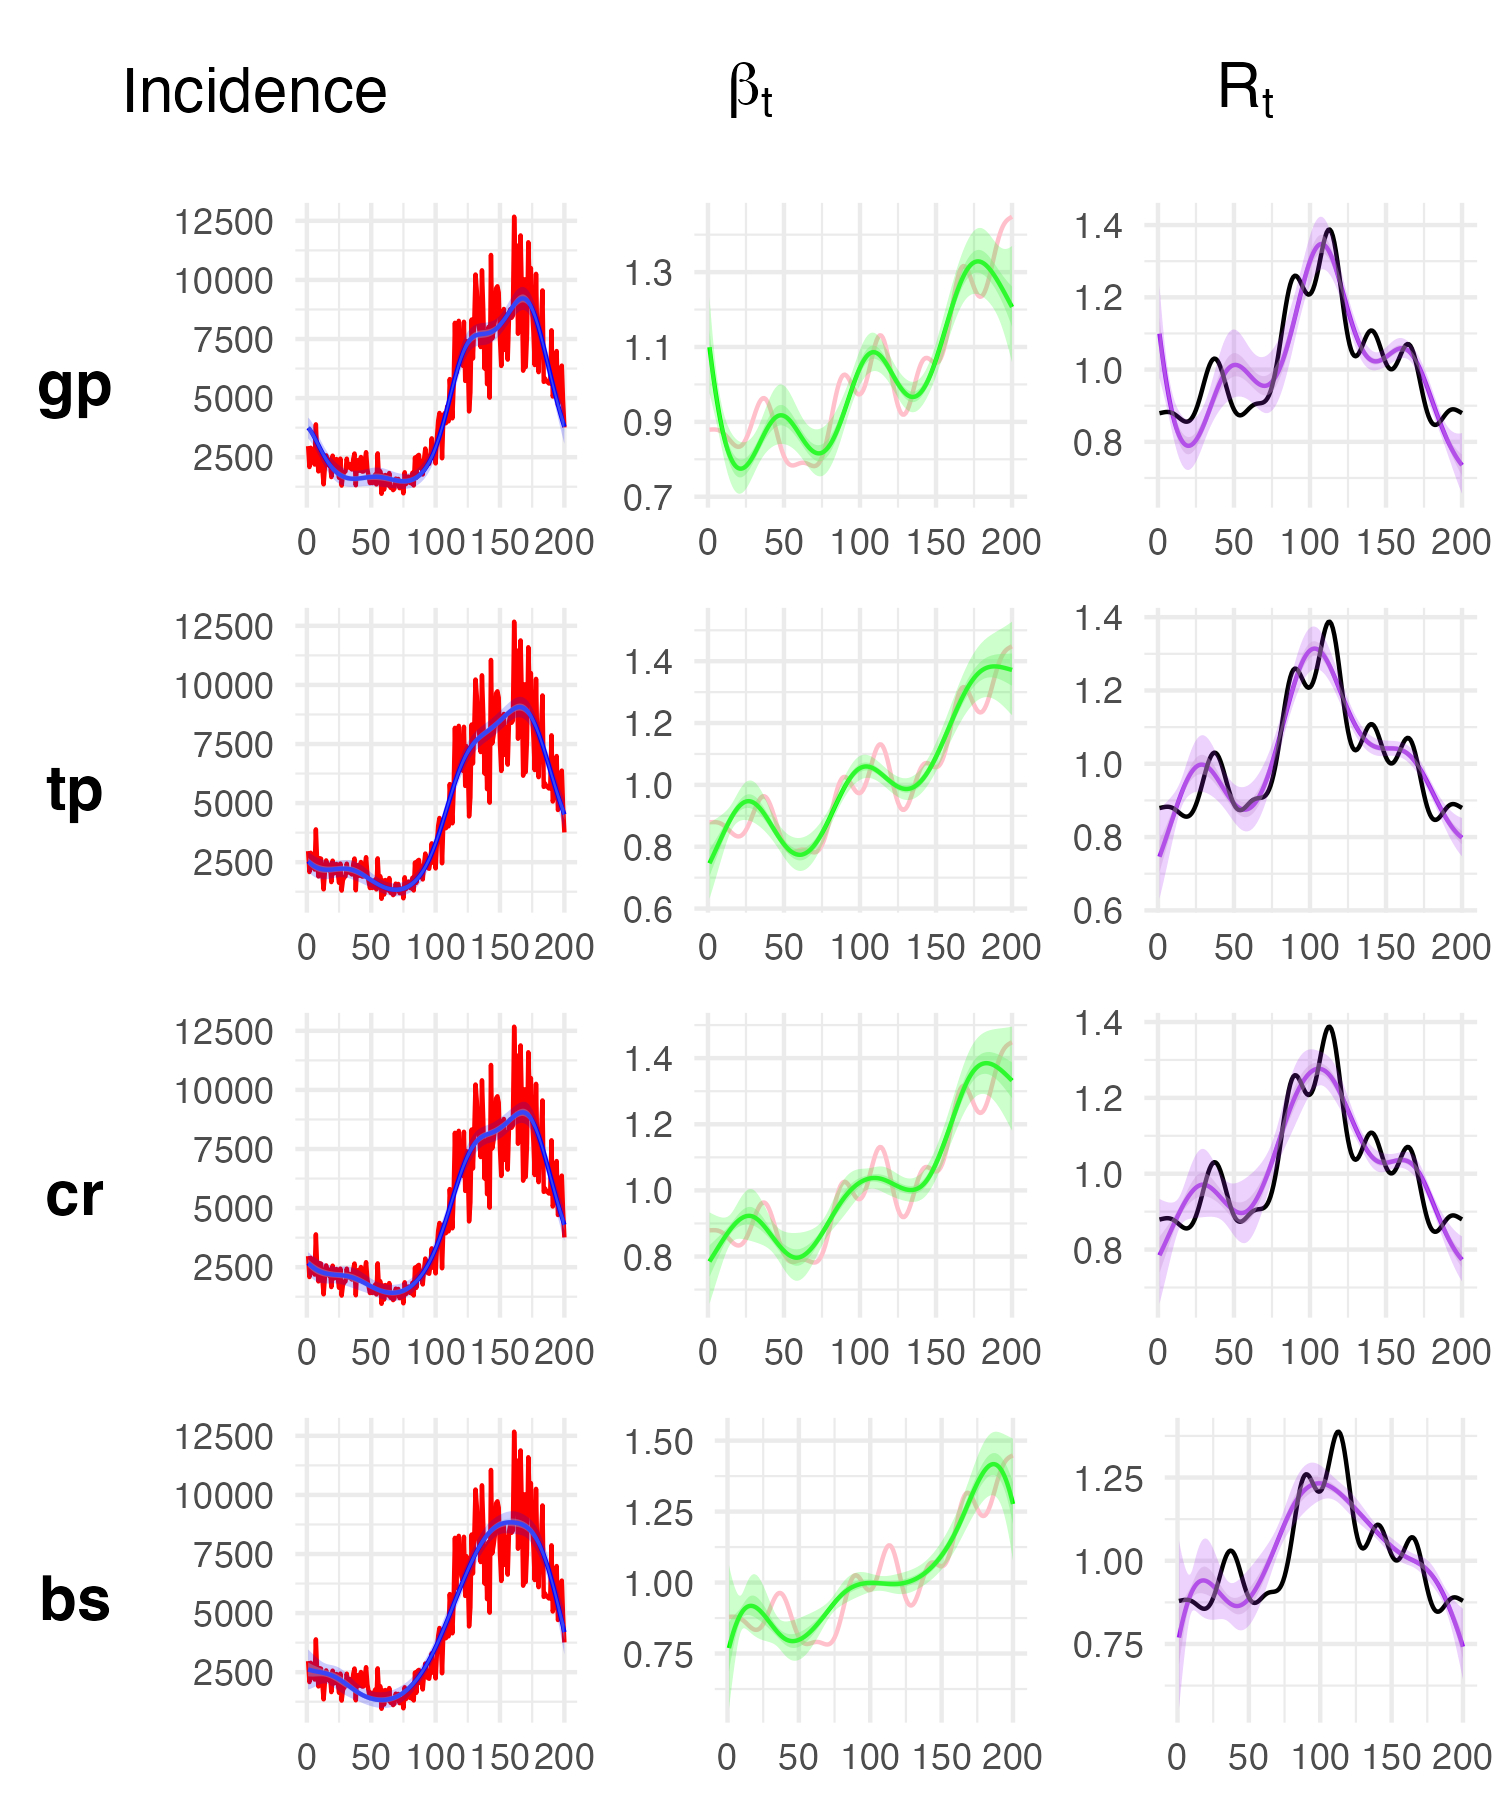
\includegraphics[width=\textwidth]{figure/Simulated/unaggregated/sim_combined_tp_k8.png}
\caption[SIRS model with simulated data (TP).]{\textbf{SIRS Model with Simulated Data (TP).} The columns represent the predicted incidence, the estimated transmission rate and effective reproduction number. The rows correspond to the different smoothing basis used to fit the model to the data. \(k=9\) knots were used to calibrate the model.}
\label{fig:sim_tp}
\end{figure}

\begin{figure}[H]
\centering
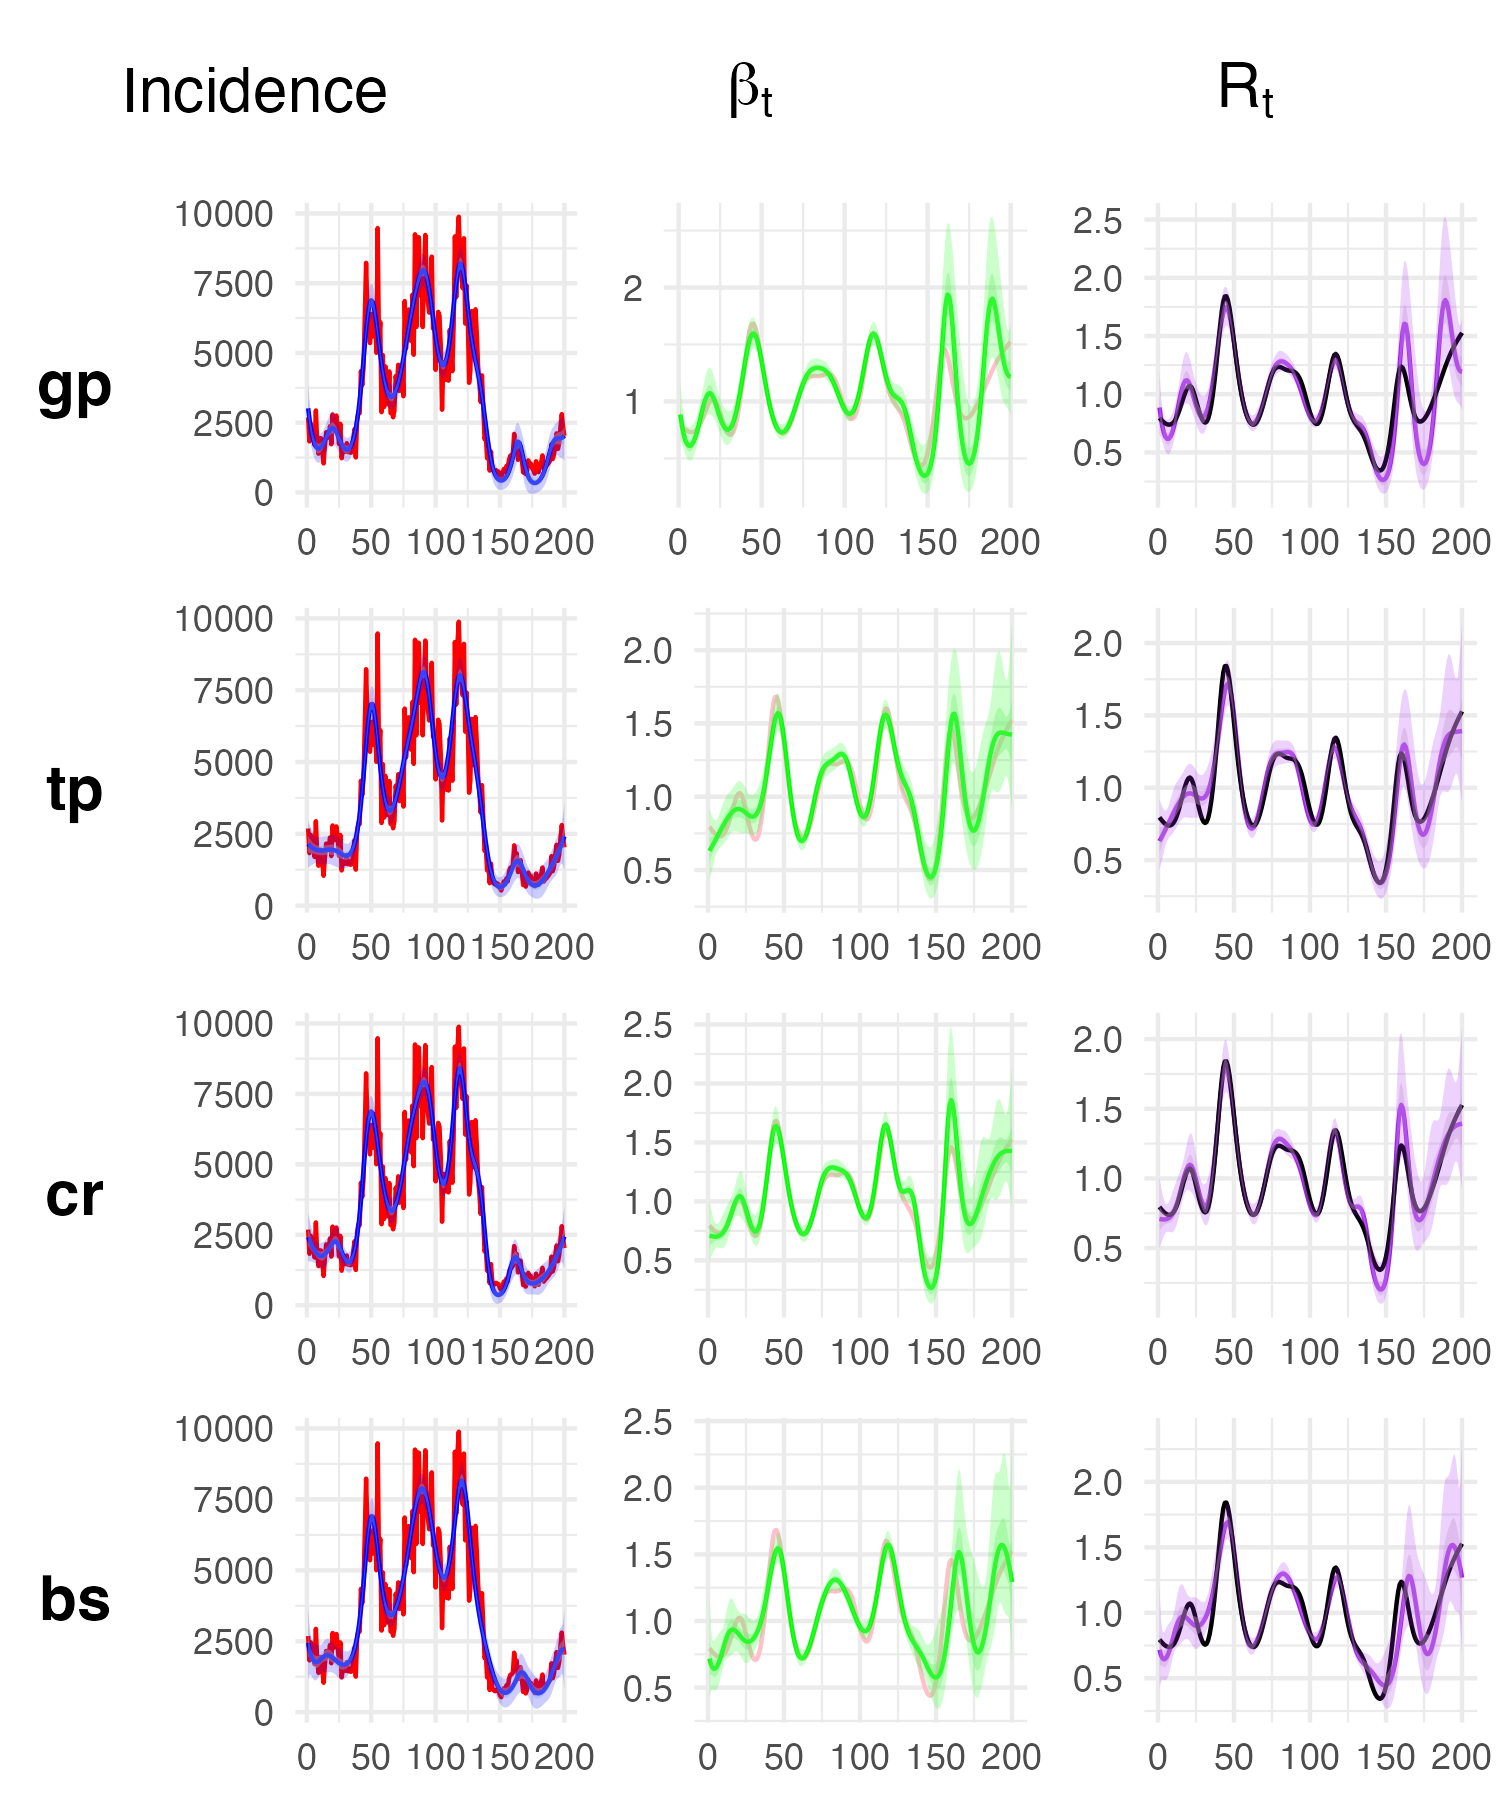
\includegraphics[width=\textwidth]{figure/Simulated/unaggregated/sim_combined_cr.png}
\caption[SIRS model with simulated data (CR).]{\textbf{SIRS Model with Simulated Data (CR).} The columns represent the predicted incidence, the estimated transmission rate and effective reproduction number. The rows correspond to the different smoothing basis used to fit the model to the data. \(k=20\) knots were used to calibrate the model.}
\label{fig:sim_cr}
\end{figure}

\begin{figure}[H]
\centering
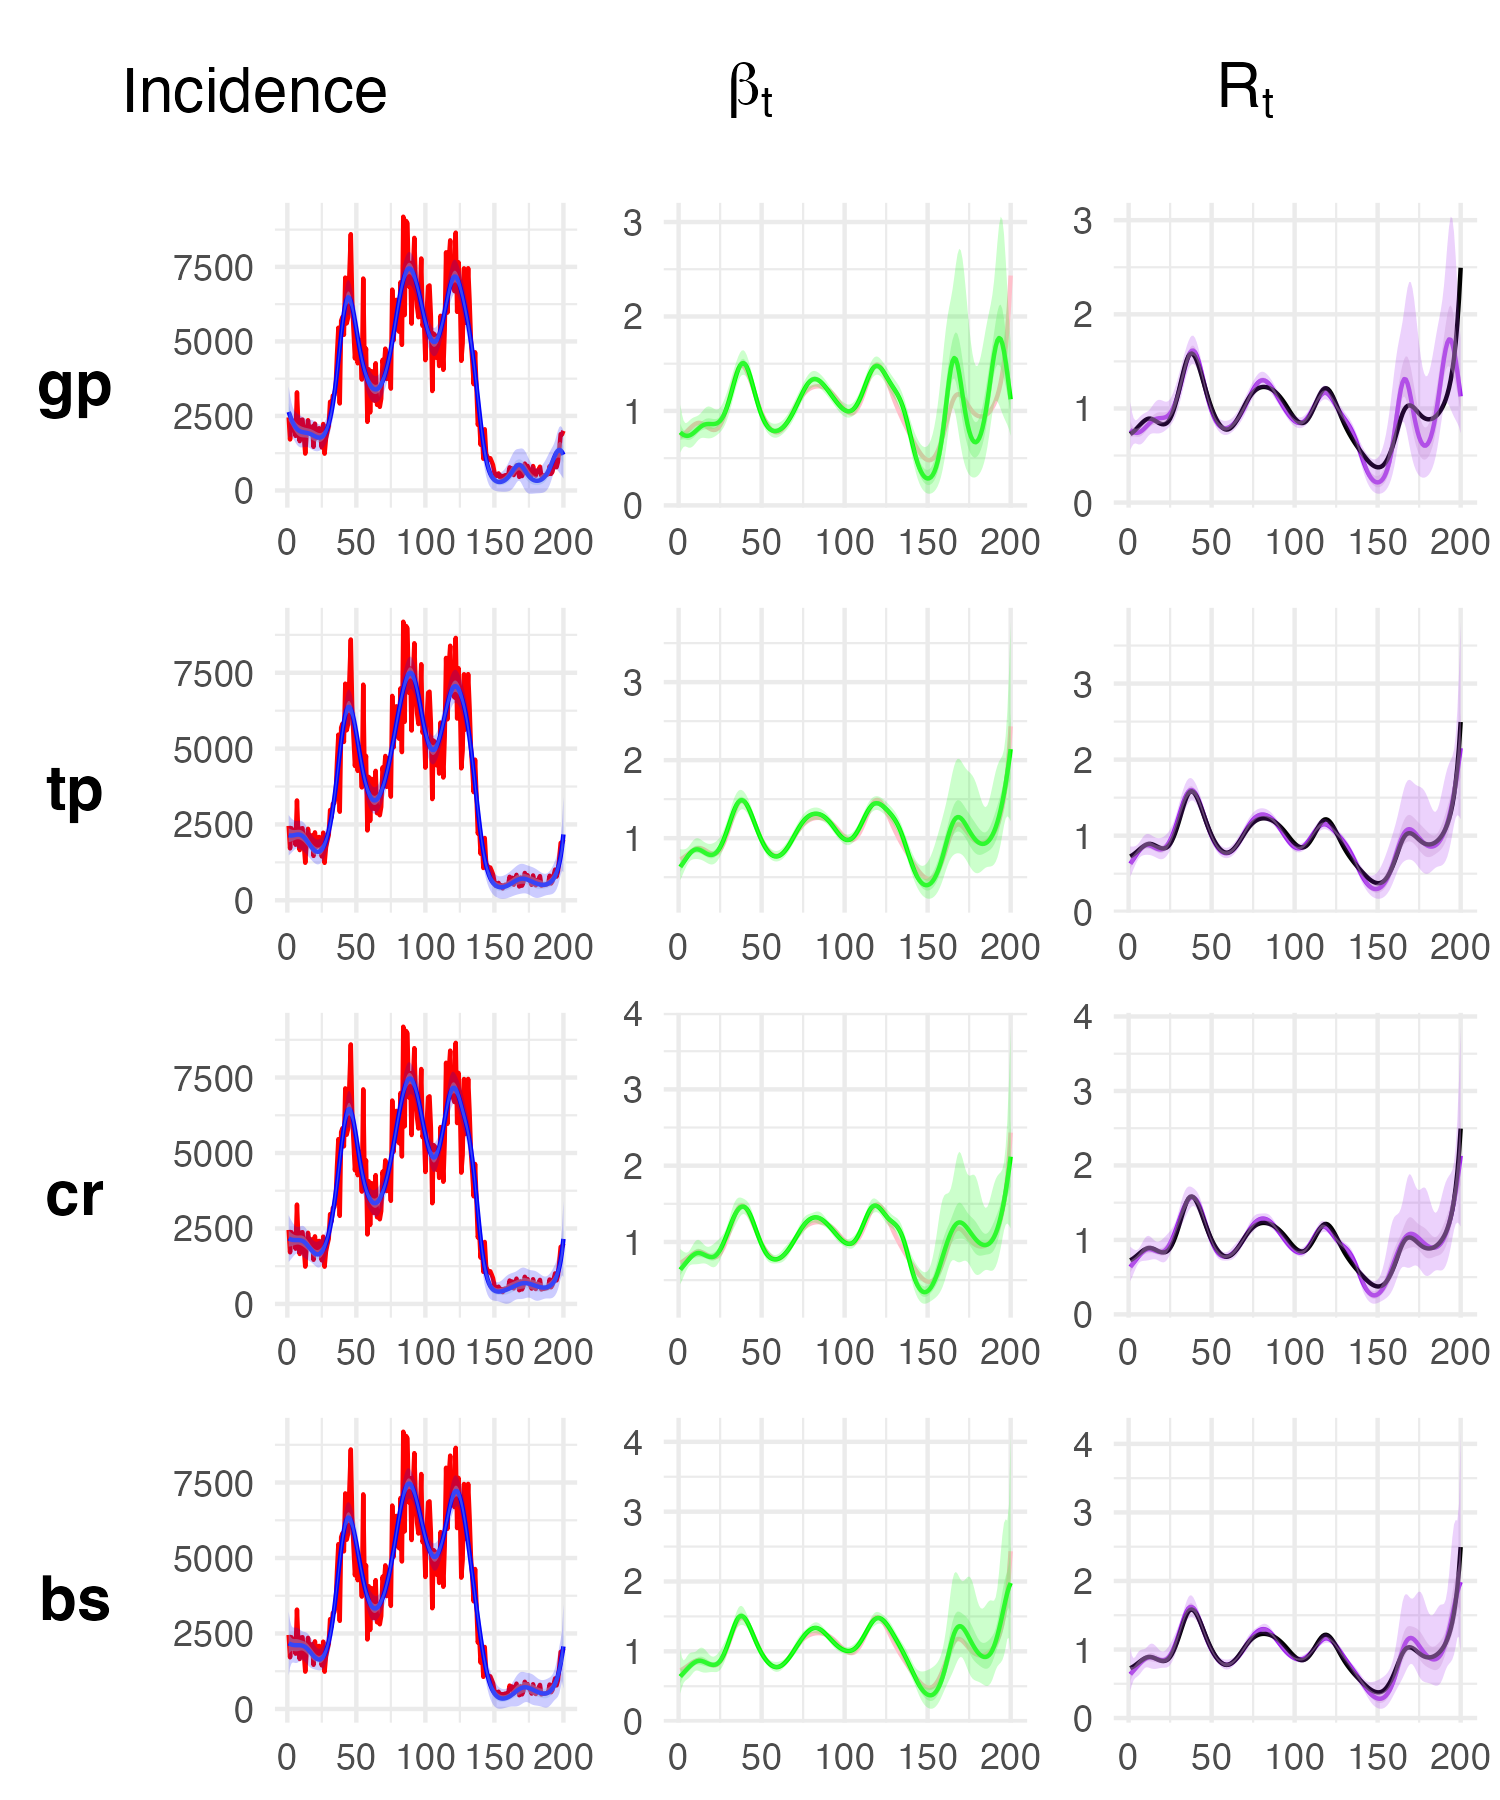
\includegraphics[width=\textwidth]{figure/Simulated/unaggregated/sim_combined_bs.png}
\caption[SIRS model with simulated data (BS).]{\textbf{SIRS Model with Simulated Data (BS).} The columns represent the predicted incidence, the estimated transmission rate and effective reproduction number. The rows correspond to the different smoothing basis used to fit the model to the data. \(k=20\) knots were used to calibrate the model.}
\label{fig:sim_bs}
\end{figure}

\begin{figure}[H]
\centering
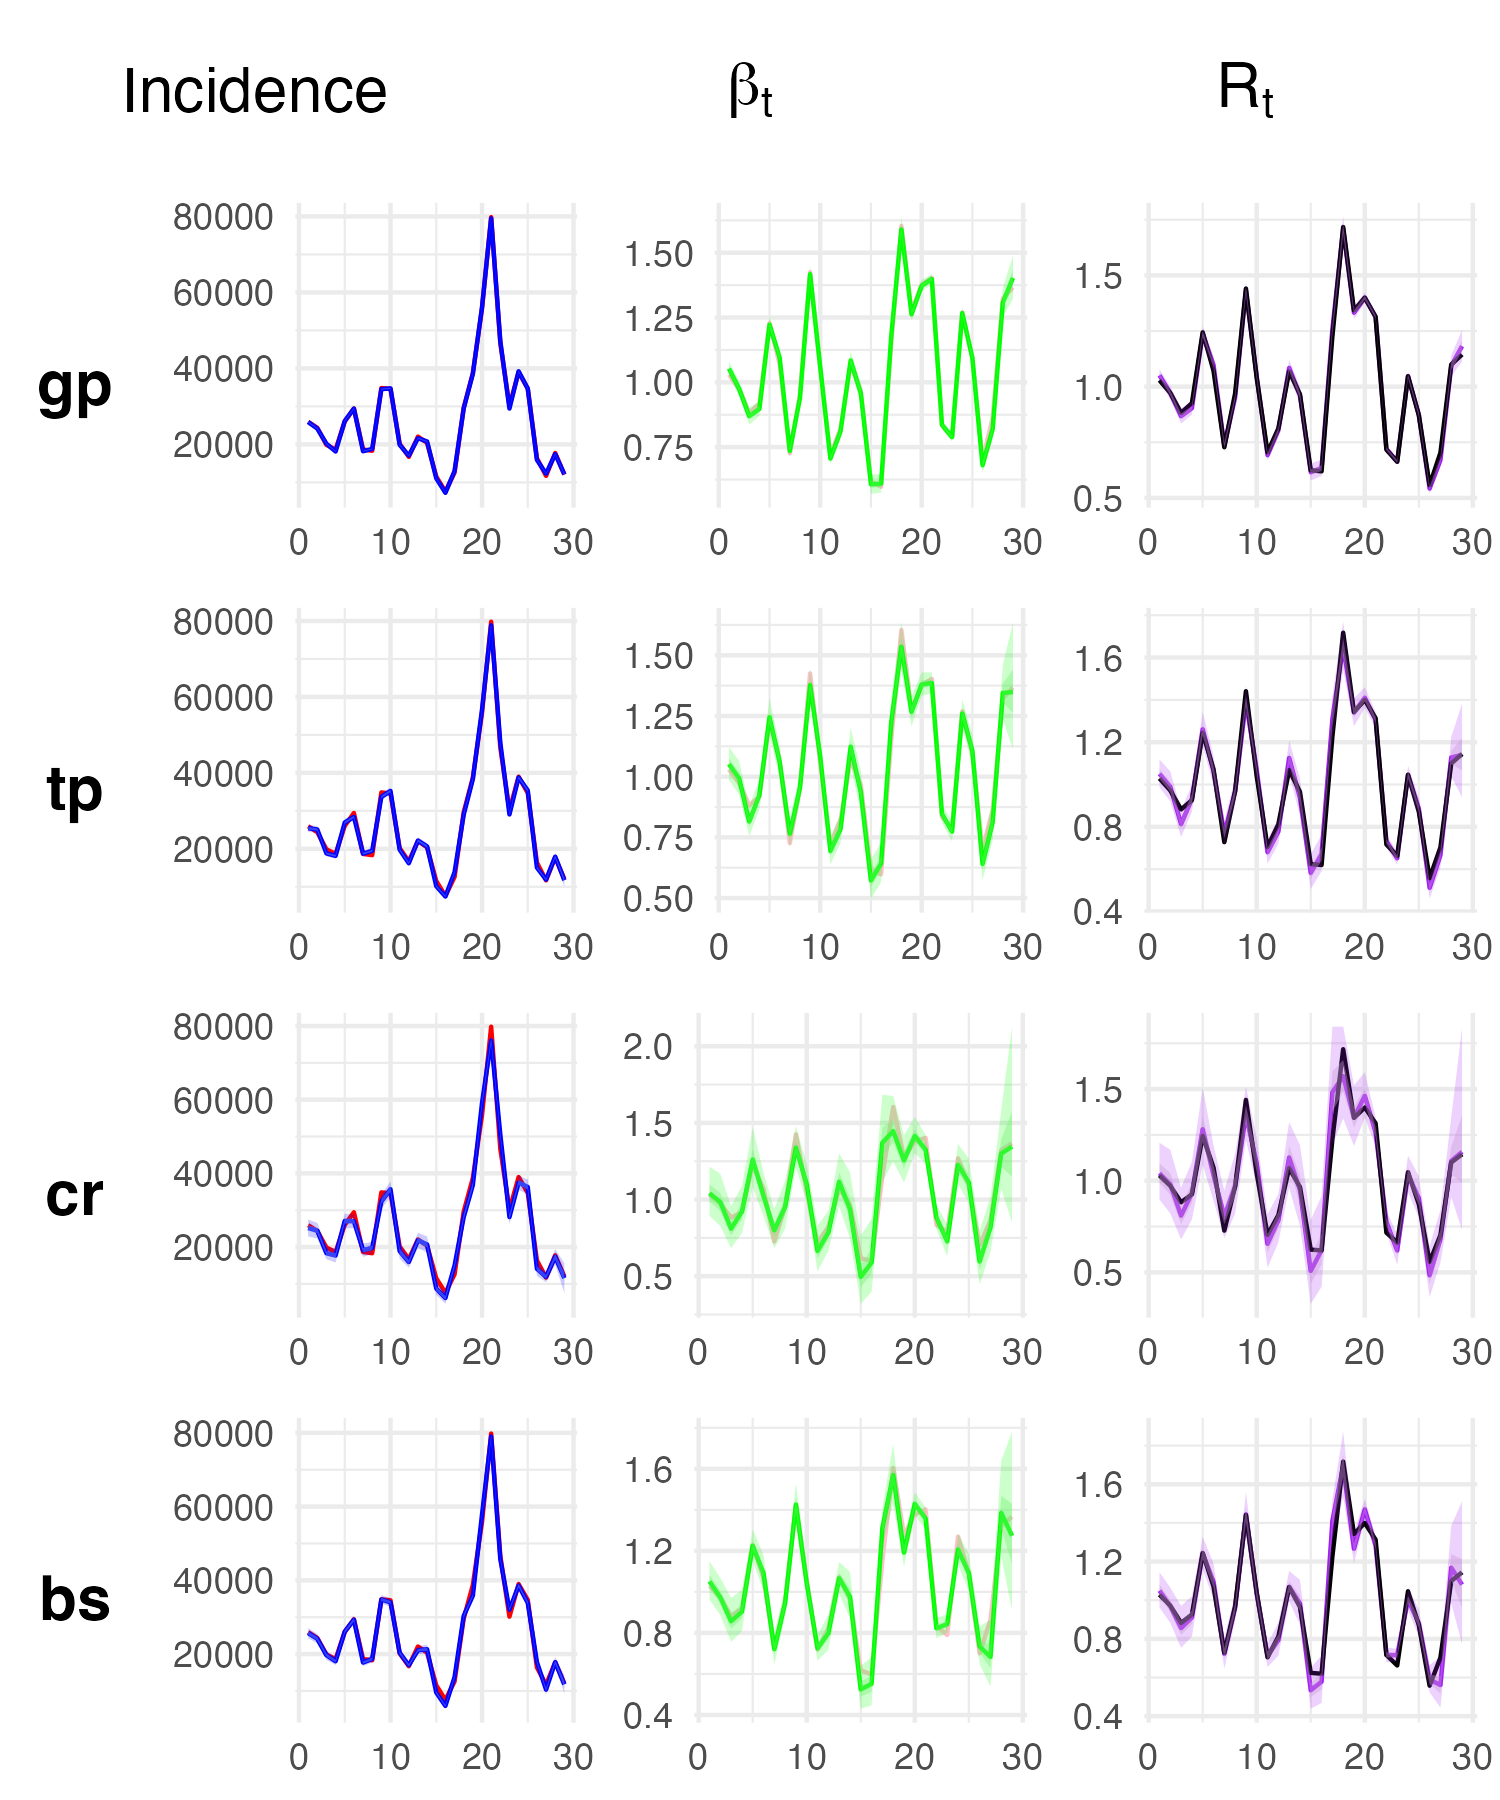
\includegraphics[width=\textwidth]{figure/Simulated/aggregated/sim_agg_combined_gp.png}
\caption[SIRS model with aggregated data (GP).]{\textbf{SIRS Model with Aggregated Data (GP).} The columns represent the predicted incidence, the estimated transmission rate and effective reproduction number. The rows correspond to the different smoothing basis used to fit the model to the data. The data was simulated on a daily scale and then aggregated to a weekly scale for model calibration. \(k=20\) knots were used to calibrate the model.}
\label{fig:sim_agg_gp}
\end{figure}

\begin{figure}[H]
\centering
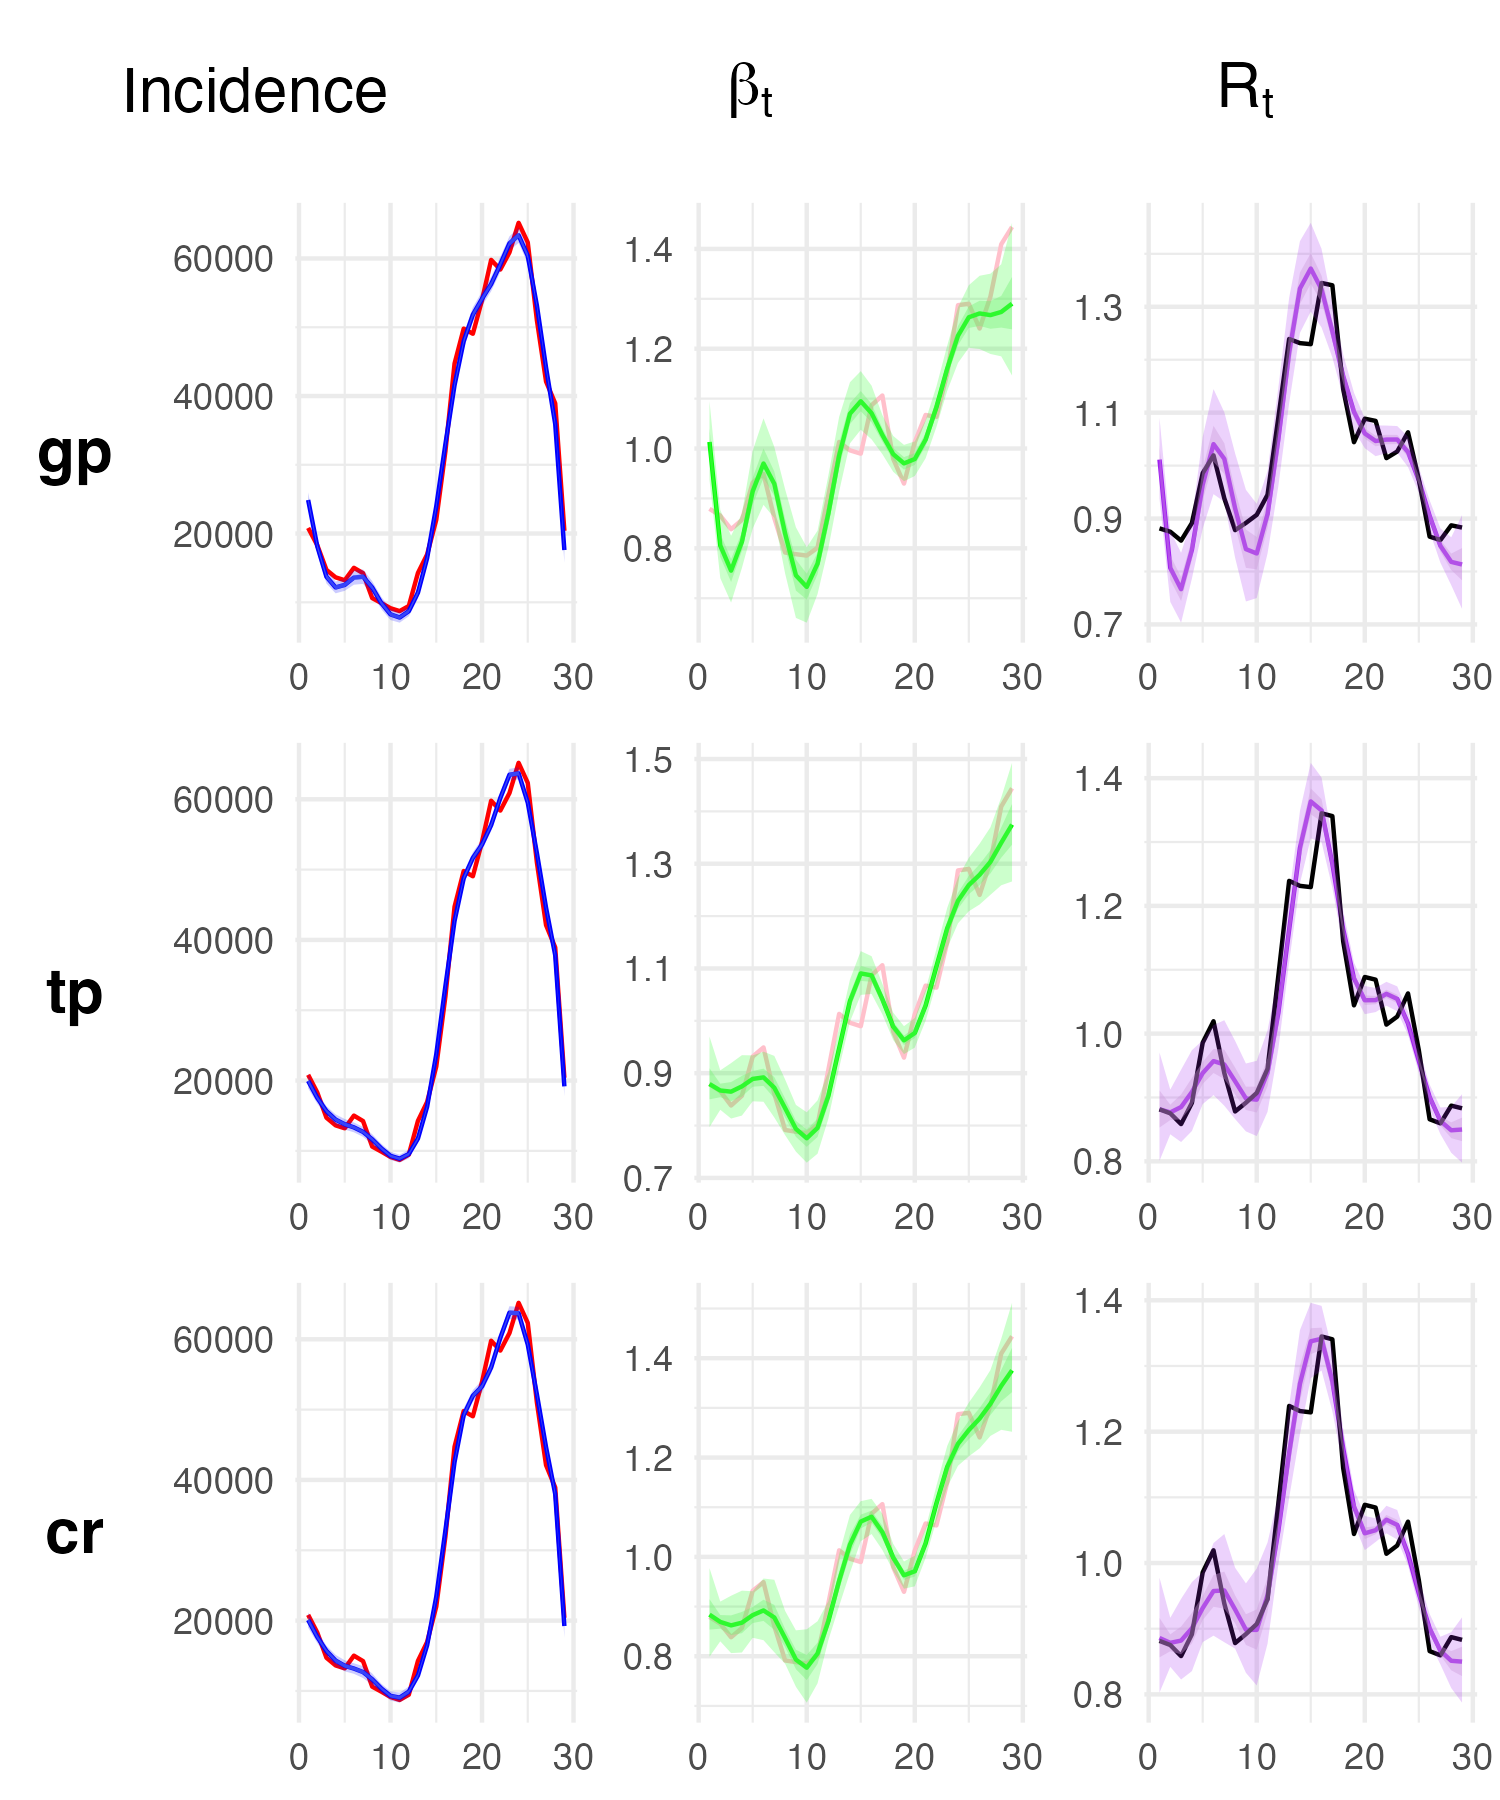
\includegraphics[width=\textwidth]{figure/Simulated/aggregated/sim_agg_combined_tp_k10.png}
\caption[SIRS model with aggregated data (TP).]{\textbf{SIRS Model with Aggregated Data (TP).} The columns represent the predicted incidence, the estimated transmission rate and effective reproduction number. The rows correspond to the different smoothing basis used to fit the model to the data. The data was simulated on a daily scale and then aggregated to a weekly scale for model calibration. \(k=9\) knots were used to calibrate the model.}
\label{fig:sim_agg_tp}
\end{figure}

\begin{figure}[H]
\centering
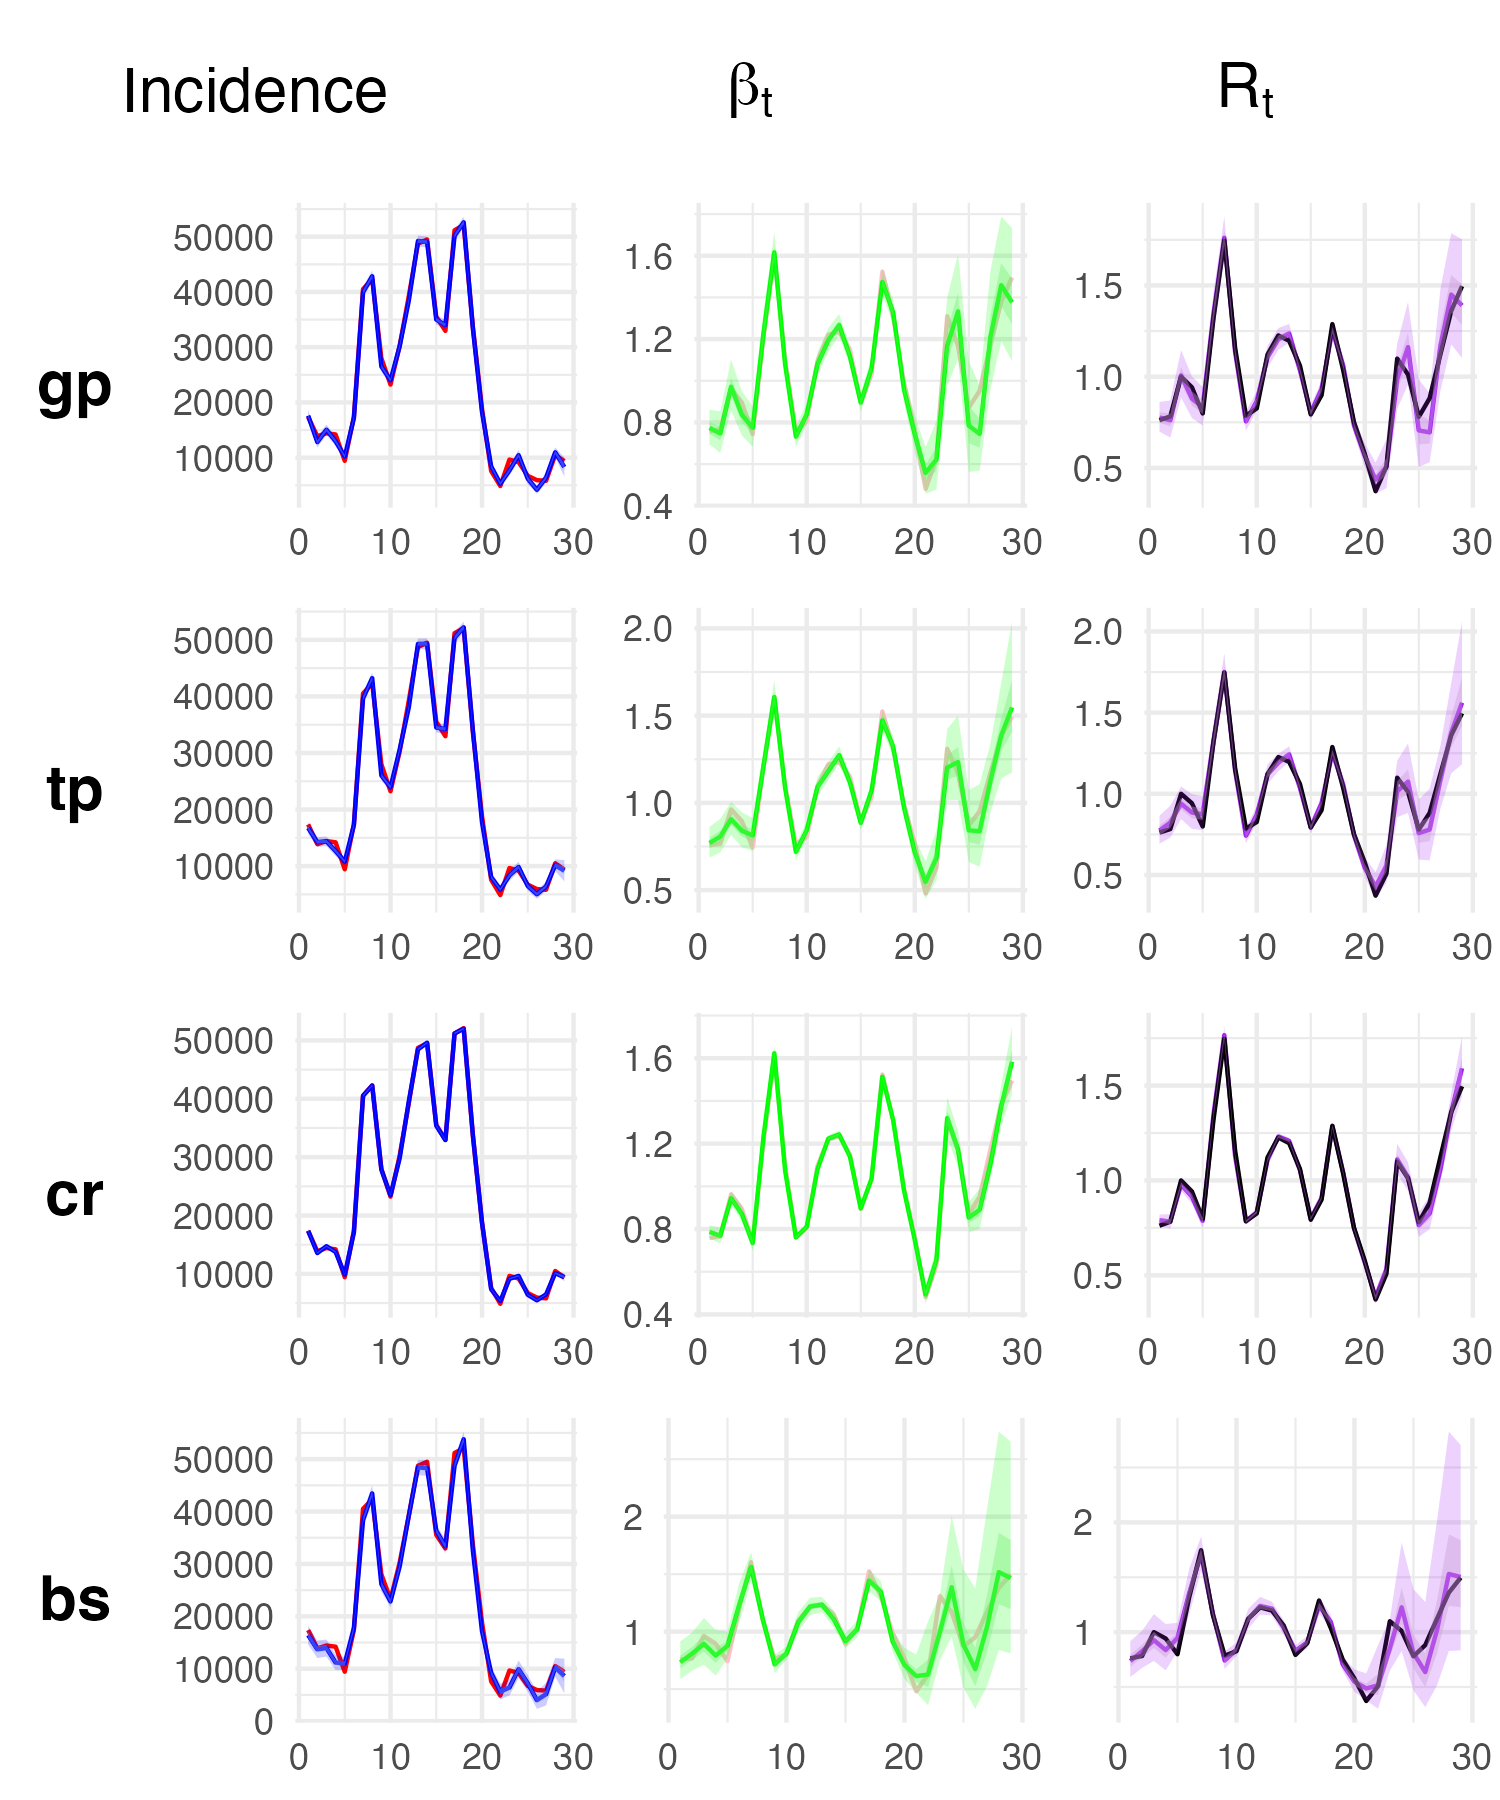
\includegraphics[width=\textwidth]{figure/Simulated/aggregated/sim_agg_combined_cr.png}
\caption[SIRS model with aggregated data (CR).]{\textbf{SIRS Model with Aggregated Data (CR).} The columns represent the predicted incidence, the estimated transmission rate and effective reproduction number. The rows correspond to the different smoothing basis used to fit the model to the data. The data was simulated on a daily scale and then aggregated to a weekly scale for model calibration. \(k=20\) knots were used to calibrate the model.}
\label{fig:sim_agg_cr}
\end{figure}

\begin{figure}[H]
\centering
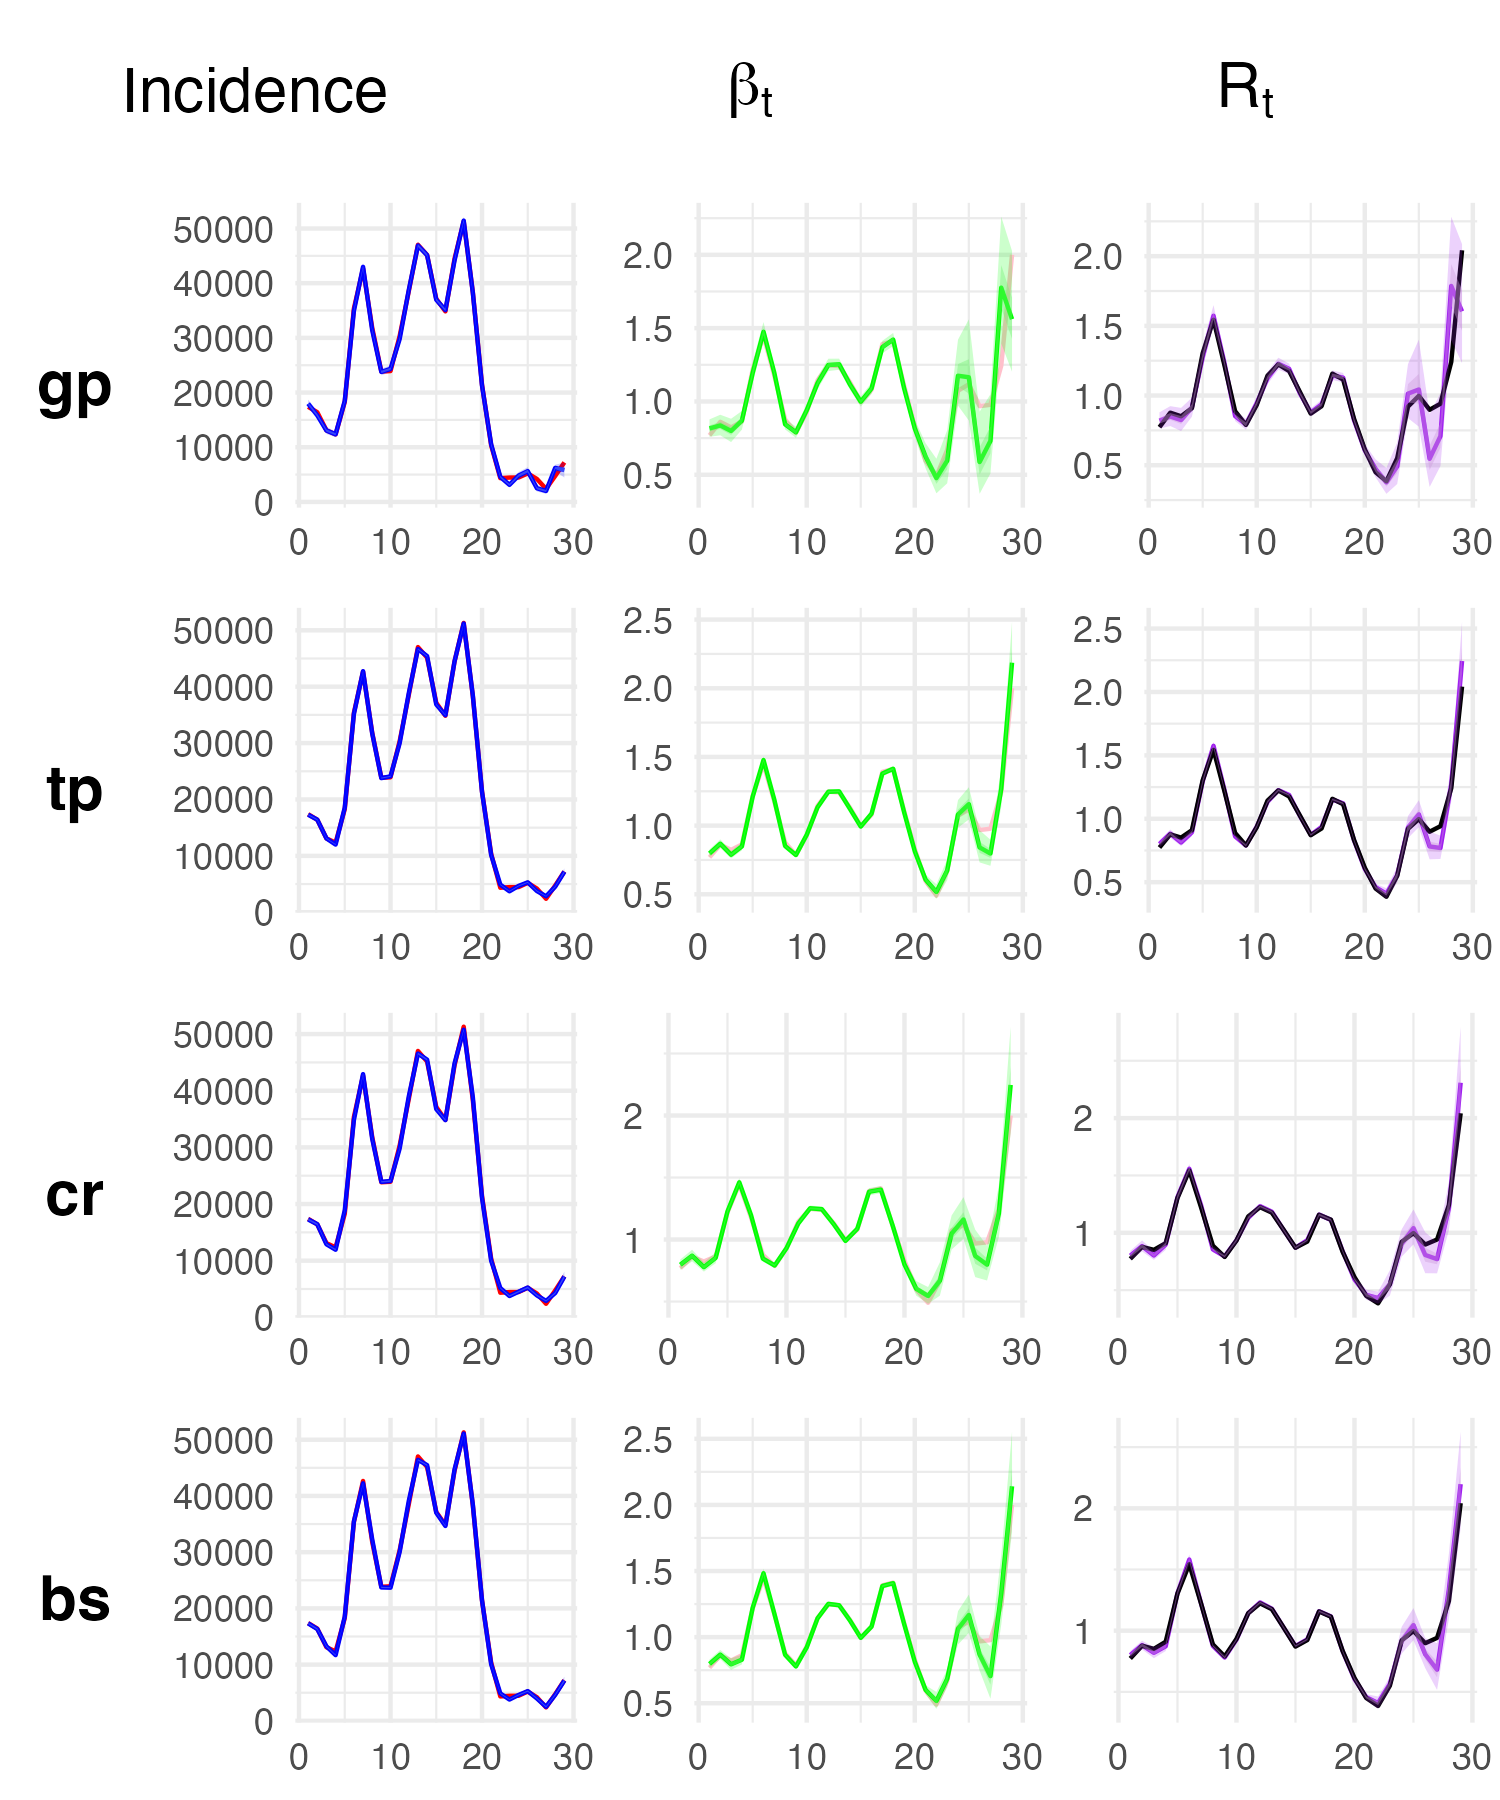
\includegraphics[width=\textwidth]{figure/Simulated/aggregated/sim_agg_combined_bs.png}
\caption[SIRS model with aggregated data (BS).]{\textbf{SIRS Model with Aggregated Data (BS).} The columns represent the predicted incidence, the estimated transmission rate and effective reproduction number. The rows correspond to the different smoothing basis used to fit the model to the data. The data was simulated on a daily scale and then aggregated to a weekly scale for model calibration. \(k=20\) knots were used to calibrate the model.}
\label{fig:sim_agg_bs}
\end{figure}

\begin{table}[!h]
\centering
\caption{\label{tab:aic-table-sim}\textbf{Conditional AIC Scores for SIRS Model with Simulated Data}. The columns represent the smoothing basis used to fit the model, while the rows indicate the basis used to generate the simulated data. The degrees of freedom are computed as the trace of the penalized smoothing matrix.}
\centering
\begin{tabular}[t]{lrrrr}
\toprule
SmoothType & gp & tp & cr & bs\\
\midrule
bs & -5.612026 & -11.41931 & -5.279962 & -4.831813\\
cr & -5.264389 & -11.30971 & -5.700246 & -4.394767\\
gp & -14.717780 & -14.83786 & -14.696820 & -14.682490\\
tp & -12.655280 & -12.84670 & -12.633240 & -12.613210\\
\bottomrule
\end{tabular}
\end{table}

\begin{table}[!h]
\centering
\caption{\label{tab:aic-table-sim-agg}\textbf{Conditional AIC Scores for SIRS Model with Simulated Data Aggregated to a Weekly Scale}. The columns represent the smoothing basis used to fit the model, while the rows indicate the basis used to generate the simulated data. The trajectories were simulated on a daily scale and then aggregated to a weekly scale for model calibration. The degrees of freedom are computed as the trace of the penalized smoothing matrix.}
\centering
\begin{tabular}[t]{lrrlr}
\toprule
SmoothType & gp & cr & tp & bs\\
\midrule
bs & -2.627495 & -2.446943 & NA & -1.028919\\
cr & -2.372933 & -1.430775 & -6.110389 & 0.067092\\
gp & -10.323190 & -10.370530 & -11.00475 & -10.313130\\
tp & -7.765698 & -7.701646 & -8.981243 & -7.467689\\
\bottomrule
\end{tabular}
\end{table}

\section{Scarlet Fever in Ontario 1929-1931}\label{scarlet}

We consider an epidemic of scarlet fever in Ontario from 1929 to 1930. The dataset comes from the International Infectious Disease Data Archives (IIDDA) {[}26{]}.

The calibration model is constructed using the basic SIR model, with an initial recovery rate of \(\gamma = 1/7\) and an initial number of infected of \(I_0 = 50\).

In Figure \ref{fig:scarlet_combined}, we show the predicted incidence, estimated transmission rate, and effective reproduction number for the best model, which uses \(k = 9\). This model employs the Ornstein-Uhlenbeck (OU), thin plate regression spline (TPRS), cubic regression spline (CR), and cyclic cubic regression spline (CC) bases for the linear smoother component. The power OU kernel for the GP basis was chosen to be consistent across all the real data examples. We observed little difference when varying the kernel type.

The shape of the estimated transmission rate and reproduction number varies across the smoothing bases for this example. The GP basis shows a positive slope as the rate of transmission reaches its maximum, whereas the TPRS, CR, and CC bases start at or very near the maximum.

In the conditional AIC scores of the four models in Table \ref{tab:aic-table-scarlet}, we see that the AIC score for the GP basis is the lowest compared to the other bases.

\begin{figure}[H]
\centering
\includegraphics[width=\textwidth, height = \textwidth]{figure/Scarlet/scarlet_combined.png}
\caption[Combined Analysis of Scarlet Fever (1929-1930)]{\textbf{Combined analysis of predicted incidence, estimated transmission rate, and effective reproduction number for weekly observed scarlet fever cases in Ontario, from 1929 to 1930.} Each column represents the predicted incidence, estimated transmission rate, and effective reproduction number, respectively. Each row corresponds to different smoothing bases used to calibrate the data, all fitted with \(k=20\) knots. The true incidence is shown in red. The covariance function of the GP basis uses a power exponential kernel, with power parameter \(\kappa = 1\) and range parameter \(\ell = 2\). The figures display 95\% and 50\% confidence intervals.}
\label{fig:scarlet_combined}
\end{figure}

\begin{table}[!h]
\centering
\caption{\label{tab:aic-table-scarlet}\textbf{Conditional AIC Scores of calibrating models with varying smoothing basis, calibrated to Ontario scarlet fever (1929-1930.} The degrees of freedom are defined as the model degrees of freedom which is computed as the trace of penalized smoothing matrix.}
\centering
\begin{tabular}[t]{ll}
\toprule
Smooth Type & cAIC\\
\midrule
gp & -12.60263\\
tp & -10.63062\\
cr & -8.483888\\
bs & -8.952309\\
\bottomrule
\end{tabular}
\end{table}

\section{Covid-19 in Ireland 2020}\label{Ireland}

Next, we fit the model to observations of the daily number of COVID-19 cases in Ireland from the onset of the outbreak, spanning February 20, 2020, to May 9, 2020. This data is sourced from the publication by Andrade and Duggan {[}27{]}.

The calibration model is constructed using the basic SIR model, with an initial recovery rate of \(\gamma = 1/6\), which is obtained from the results of Park et al. {[}28{]}.

Figure \ref{fig:ireland_combined} presents the results of the best models, which utilize the GP, TPRS, and CR smoothing bases. The BS basis functions exhibited extremely large uncertainty estimates, so we did not include the results. All bases displayed an excellent fit to the observed incidence data with appropriately sized uncertainty estimates.

Table \ref{tab:aic-table-ireland} provides the conditional AIC scores.

The model's sensitivity to changes in the starting value of \(\gamma\) (ranging from 7 to 14 days) does not alter the shape of the functional form of \(\beta\), but it changes the amplitude of the peak, leading to an increase in \(R_t\). Increasing the variance of the log-normal prior on \(\gamma\) causes the model to tend to select a larger \(\gamma\). However, this also results in a dramatic increase in uncertainty estimates. We observed that when the starting value of \(\gamma\) is lowered and the variance of the log-normal prior is increased simultaneously, the model still predicts larger values of \(\gamma\).

Andrade and Duggan (2022) used COVID-19 data to infer the effective reproduction number by employing an SEIR model with three different data-generating processes for the transmission rate. One of the processes they used was Geometric Brownian Motion (GBM). GBM is similar to the Ornstein-Uhlenbeck (OU) process that we used, but it is non-stationary, non-mean-reverting, and the response is log-normally distributed. In our thesis, we implemented the OU process as a special case of a Gaussian Process (GP) with an exponential covariance function. By viewing the OU process as a GP, we focus on the joint distribution of values at different times, characterized by the mean and covariance functions. These functions describe the decay rate of the covariance and the process variance, respectively, emphasizing the correlation structure. Computationally, this approach allows us to use linear algebra. Andrade and Duggan define the transmission rate using GBM formulated as an SDE. They also assume that the response, the incidence data, follows Poisson and Negative Binomial distributions. Additionally, they use Apple mobility data to adjust the transmission rate by assuming that the effect of social distancing is correlated with the transmission rate.

We compared our results, using the OU process basis for our linear smoother, with those of Andrade and Duggan. They aggregated their incidence data to a weekly scale to account for irregularities in daily reporting. We implemented this by computing the trajectory on a daily scale, aggregating the predicted incidence to a weekly scale, and then fitting the model to the weekly aggregated observed data. The daily trajectory of the transmission rate and reproduction number estimates are then averaged over each week.

The predicted incidence fits the data well, with very reasonable uncertainty bounds, and the shape is very similar to Andrade and Duggan's results. The estimated transmission rates, ignoring the first week in our plots, both show approximately the same shape, an exponential decay. The magnitude of the transmission rate is about twice as large for Andrade and Duggan compared to our results. The estimated effective reproduction number, which is the transmission rate scaled by the recovery rate and the proportion of susceptibles at any time \(t\), also shows a similar pattern. Although Andrade and Duggan compute an analytical expression for the basic reproduction number and we compute ours as the transmission rate scaled by the recovery rate, we both scale the basic reproduction number by the ratio \(\frac{S_t}{N_t}\) to obtain the effective reproduction number. Most notably, we observe that the estimated effective reproduction number has not only the same shape as Andrade and Duggan's but also a similar magnitude. The uncertainty estimates are tighter in our model, but our model is simpler.

\begin{table}[!h]
\centering
\caption{\label{tab:aic-table-ireland}\textbf{Conditional AIC Scores of calibrating models with varying smoothing basis, calibrated to Ireland Covid-19 (2020).} The degrees of freedom are defined as the model degrees of freedom which is computed as the trace of penalized smoothing matrix.}
\centering
\begin{tabular}[t]{ll}
\toprule
Smooth Type & cAIC\\
\midrule
gp & -8.594023\\
tp & -6.867158\\
cr & -5.810518\\
\bottomrule
\end{tabular}
\end{table}

\begin{figure}[H]
\centering
\includegraphics[width=\textwidth, height = \textwidth]{figure/Ireland/ireland_combined.png}
\caption[Combined Analysis of Covid-19 in Ireland (2020)]{\textbf{Combined analysis of predicted incidence, estimated transmission rate, and effective reproduction number for observed Covid-19 cases in Ireland, 2020.} The data is given on a daily scale, and the trajectory is simulated daily but aggregated to a weekly scale for fitting the model. Each column represents the predicted incidence, estimated transmission rate, and effective reproduction number, respectively. Each row corresponds to different smoothing bases used to calibrate the data, all fitted with \(k=7\) knots. The true incidence is shown in red. The covariance function of the GP basis uses an exponential kernel function, which makes the basis an Ornstein-Uhlenbeck process, with exponent parameter \(\kappa = 1\) and range parameter \(\ell = 2\). The figures display 95\% and 50\% confidence intervals.}
\label{fig:ireland_combined}
\end{figure}

\section{Measles London UK 1944-1984}\label{Measles}

We now present a more challenging problem than the previous examples. We consider weekly observed measles cases in London, UK, from 1944 to 1984. This dataset was first utilized in a publication by David Earn et al. {[}29{]}.

The calibration model is constructed using the basic SIR model. The starting value for the recovery rate is \(\gamma = 1/8\), aligning with the initial value used in {[}29{]}. A key assumption we make is that the total population remains constant over time. This is due to the nature of the SIR model, which does not account for a time-varying total population component. We fixed the total population to \(N = 8,615,050\), which is the population of London at the start of this dataset. This assumption is reasonable, as the population of London has fluctuated between six and ten million from then until the present day. However, since the disease predominantly affects children, a more sophisticated model could include a time-varying total population component, partitioned according to age and weighted by the incidence rate per age demographic. We initialize the number of infected individuals at \(I_0 = 250\).

The full dataset extends to 1994, but we had difficulty tuning the model to fit the last decade. During this period, the observed incidence was relatively flat compared to the previous years. We observed that the calibrated model inflated the predicted transmission rate to unreasonable levels. By truncating the last decade, reducing the observations from 2,660 to 2,140, we were able to calibrate the model more effectively.

We exclusively present the results for a Gaussian process basis for the linear smoother component of the model. Other smoothing bases were tested, but the optimizer failed to converge for more than 100 to 200 observations, as the Newton-Raphson method failed to find a minimum. In Figure \ref{fig:Measles_trans}, we show the predicted incidence, transmission rate, and effective reproduction number for the SIR model with a Gaussian process basis for the linear smoother component. The covariance function is the exponential kernel with a range parameter \(\ell = 20\). Other kernels, such as the Matérn function, were tested by iterating over different range parameters \(\ell = 30, 40, 50\). The resulting models showed little difference in optimized parameter values and conditional AIC scores. For simplicity, we present the parsimonious model with the simplest kernel function and the smallest range parameter. Each model took about 20 minutes to fit.

Figure \ref{fig:Measles_trans} displays the optimized values of the parameters in the calibrated model and their uncertainty measurements. These are the log transformed values. Exponentiating, the partial prior on \(\gamma\) produced an optimal value of \(\frac{1}{11.84}\).

\begin{figure}
\centering
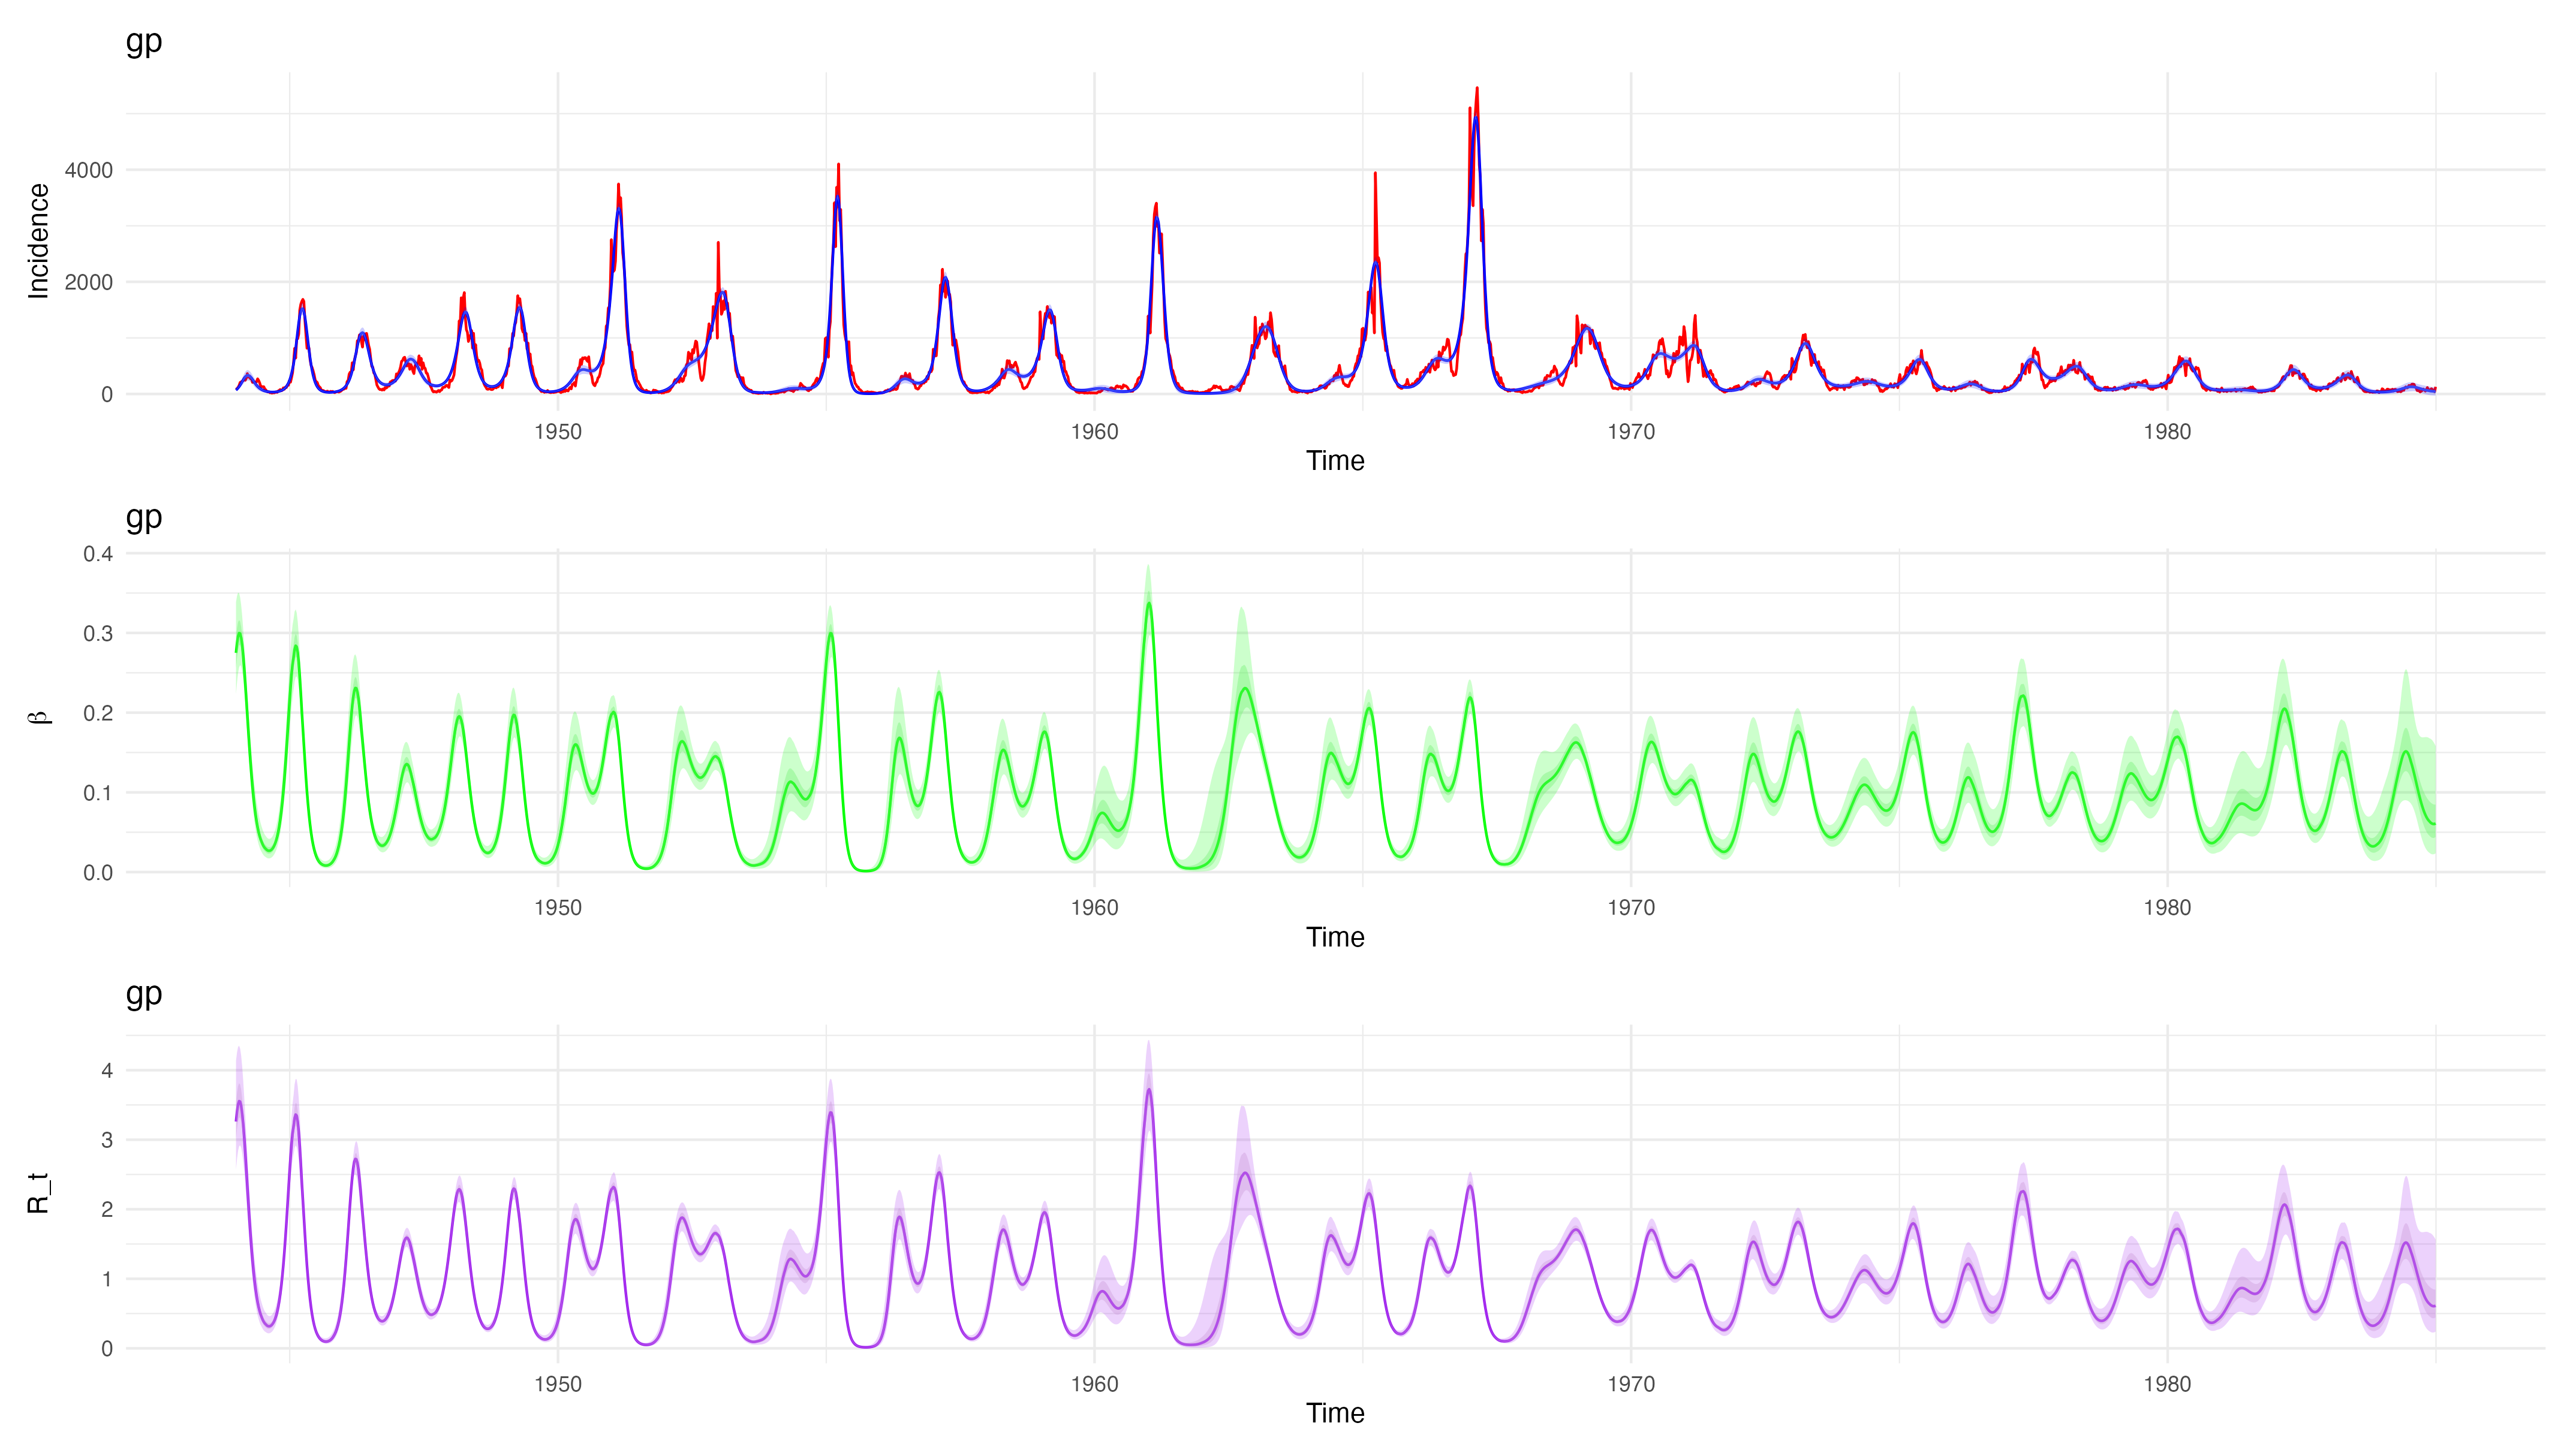
\includegraphics[width=\textwidth, height = \textwidth]{figure/Measles/Measles_combined_plot.png}
\caption[Combined Analysis of Measles in London, UK, (1944-1984)]{\textbf{Predicted incidence and estimated transmission rate and effective reproduction number for weekly observed measles cases in London, UK, from 1944 to 1984 using a Gaussian Process smoother.} The linear smoother component of the semi-mechanistic compartmental model employs an Ornstein-Uhlenbeck (OU) process with a range parameter \(\ell = 20\) and \(k = 100\) knots. The model estimates a recovery rate of approximately \(\gamma = 11.84\) days and an initial number of infected individuals of approximately \(I_0 = 250\). The figures display 95\% and 50\% confidence intervals.}
\label{fig:Measles_trans}
\end{figure}

\chapter{Discussion}\label{Discussion}

This thesis presents a method for formulating infectious disease compartmental models without relying on unjustified biological assumptions about the disease transmission process, as required by fixed or parametric models. By integrating this approach into the \texttt{macpan2} and \texttt{TMB} frameworks, we provide a user-friendly way for modelers to fit models, select the best model, and infer estimates of latent variables over time. We accomplished this by adapting the general methodology of Simon Wood {[}7{]} and utilizing it in conjunction with the aforementioned model formulation tool and optimization engine.

Our work differs from that of Simon Wood by making this methodology accessible to quantitatively minded modelers who may not be experts in nonlinear optimization and smoothing theory. This was achieved because \texttt{macpan2} is designed from a software-engineering perspective. It wraps all the necessary \texttt{C++} code to interact with \texttt{TMB} in an \texttt{R} wrapper, eliminating the need for modelers to write bespoke optimization code, which can be a significant barrier to using such models.

Through simulation studies, we demonstrated the efficacy of penalized smoothing parameter estimation. The \texttt{mgcv} package greatly facilitated the construction of low-rank smoothing bases and penalty matrices for a given domain and model granularity. We compared different smoothing bases, evaluating their performance based on uncertainty estimates, AIC scores, and the shapes of the estimated functions.

We successfully fitted the models to real-world incidence data, with the goodness of fit controlled by smoothness inferred through penalization. These results indicate that this methodology can be beneficial to any modeler wishing to estimate a time-varying latent variable by inferring the shape of an unknown function. Although we focused on modeling infectious disease with unknown transmission rates and reproduction numbers, it seems reasonable that this approach can be applied to arbitrary compartmental models with unknown time-varying functions. This methodology can even extend to dynamic ecological models formulated using compartmental models.

The models were effective in inferring fixed parameters. Unlike most epidemiological studies {[}30,31{]}, we did not fix the recovery rate and the initial number of infected individuals to their initial values. Instead, we introduced flexibility by applying a sharp partial Bayesian log-normal prior, treating the quantile of this prior as a parameter calibrated using the data. For future research, a fully Bayesian approach could be adopted by specifying prior distributions for both the mean and variance of the log-normal distribution.

The relative performance of different smoothing bases across all examples can be analyzed. In all examples (subsections \ref{simulation}, \ref{scarlet}, \ref{Ireland}, and \ref{Measles}), the Gaussian process (GP) regression smoothing basis consistently proved to be the best in several respects. The GP basis was the most robust to increases in effective degrees of freedom. Tables \ref{tab:aic-table-sim}, \ref{tab:aic-table-scarlet}, and \ref{tab:aic-table-ireland} show that during model fitting, selecting model complexity by adjusting the smoothing parameter \(\lambda\) resulted in an increase in the conditional AIC score. Checking the resultant effective degrees of freedom for the fitted models across different bases, the GP basis consistently showed the lowest values. This indicates that the GP basis, in conjunction with the \texttt{nlminb} optimizer used by \texttt{TMB}, is able to find the best smoothing parameter value compared to other bases. Additionally, across all datasets, the GP basis performed best or near-best. Notably, it was the only model capable of fitting the large measles dataset. Our conclusion is that using this methodology, a GP basis is generally an effective choice.

The SIR and SIRS compartmental models used in this work are basic compartmental models. Theoretically, a compartmental model can be as complex as the modeler wishes, but in practice, certain assumptions are made to make the fitting process tractable. The models we used serve as toy examples that demonstrate the proof of concept for the efficacy of the methodology presented in this thesis.

In contrast, more realistic compartmental models can be highly complex, including numerous compartments (or nodes) and connections (or edges) between them, each with associated parameters or unknown functions that need to be estimated. These models can account for various factors such as different stages of infection, varying rates of transmission, recovery, and immunity, as well as heterogeneity in the population.

Despite their simplicity, our models effectively demonstrate the potential of the methodology. However, they do not capture the full complexity of real-world scenarios, where the intricate dynamics of disease spread necessitate more sophisticated models. By starting with these simpler models, we establish a solid foundation for understanding and validating the methodology before potentially extending it to more complex and realistic compartmental models in future research.

Assuming the unknown function is simply linear, as done in this thesis (when the smoother parameter is fixed for each iteration), is a step towards constructing more complex forms of the unknown function. If the modeler wishes to incorporate biological information about the transmission process into the model, they might impose qualitative conditions on the unknown function. For instance, if the unknown function is assumed to be monotone, the modeler can impose specific conditions of monotonicity and boundedness on the smoother. Extending this methodology to include specific constraints on the smoother allows the literature to guide the shape of the fitted unknown function by applying qualitative constraints to the smoothing functional.

In summary, this thesis presents a proof of concept for estimating time-varying unknown functions in deterministic compartmental models. There are many possible avenues for extension, some of which we have discussed above. More generally, this thesis suggests that it should be possible to adapt this methodology to be used within any optimization framework that fits mixed models by using the theory of the duality of smooths and random effects, to rewrite the smoothing basis as random effects matrices, as discussed in subsection \ref{The-duality-of-smooths-and-random-effects}. Another avenue of research is to estimate more than one unknown function. All the methods presented here are easily extensible to fitting models to data with more than one unknown function, each with its own smoothing parameter. Wood {[}32{]} and Gu {[}16{]} describe how to formulate models with more than one smoothing parameter.

\appendix

\chapter{Mathematical derivations}\label{Appendix}

\section{Matrix formulations and basis functions for cubic smoothing splines}\label{A1}

The following is adapted from the proof in {[}12{]} for deriving the basis functions and matrix elements of a natural cubic spline. We extract the key equations and essential conceptual steps, omitting computational details and expanding on the equations' meanings. This approach highlights how the natural boundary conditions and continuity conditions at the knots constrain the solution of the Euler-Lagrange equation over each continuous interval to be a cubic spline which vanishes outside the endpoints of its domain.

To determine the function \(f\) that minimizes

\[
J_{2}(f) = \sum_{i=1}^n (y_i - g(x_i))^2 + \lambda \int g''(x)^2 \, dx,
\]
we apply the Euler-Lagrange equation to a more general functional form \(J(x) = \int L(x, x', x'', t) \, dt\). The Euler-Lagrange equation for this functional becomes:

\begin{equation}
\frac{\partial L}{\partial x} - \frac{d}{dt} \frac{\partial L}{\partial x'} + \frac{d^2}{dt^2} \frac{\partial L}{\partial x''} = 0.
\label{eq:expanded Euler-Lagrange equation}
\end{equation}

When the function \(f(x)\) extends beyond the range of the data points, or knots, we avoid imposing fixed boundary values for \(x\) and \(x'\) at the domain boundaries (i.e., \(x(t_a)\), \(x(t_b)\), \(x'(t_a)\), and \(x'(t_b)\)). Instead, we use \emph{natural boundary conditions}.

Natural boundary conditions are designed to ensure that the contributions from the boundary conditions to the first-order variation \(\delta J = J(x + \delta x) - J(x)\) vanish, thus optimizing the solution. In standard scenarios, fixed values might be set for \(\delta x\) and \(\delta x'\), where \(\delta\) represents an infinitesimal change. However, this could potentially lead to undesirable behavior at the boundary points, especially outside the region defined by the knots.

From the application of the Euler-Lagrange equation \ref{eq:expanded Euler-Lagrange equation} and the principle that the first-order variation \(\delta J\) should vanish at the optimal solution, we derive two critical \emph{natural boundary conditions}:

\[
\frac{\partial L}{\partial \dot{x}} - \frac{d}{dt} \frac{\partial L}{\partial \ddot{x}} = 0 \quad \text{and} \quad \frac{\partial L}{\partial \ddot{x}} = 0,
\]
where these conditions are each evaluated at \(t_a\) and \(t_b\). These conditions help ensure that the function \(f(x)\) not only fits the data within the knot range but also behaves optimally at the boundaries without artificial constraints.

Now, we can express Equation \ref{eq:min_smoothness_obj} in a variational form as follows:
\[
J = \sum_{n=0}^{N-1} w_n (y_n - x(t_n))^2 + \lambda \int_{t_a}^{t_b} x''(t)^2 \, dt,
\]
where the Lagrangian \(L\) is defined by:
\[
L = \sum_{n=0}^{N-1} w_n(y_n - x(t))^2 \delta(t - t_n) + \lambda x''(t)^2.
\]

Applying the Euler-Lagrange equation to this formulation yields:
\begin{equation}
\frac{\partial L}{\partial x} - \frac{d}{dt} \frac{\partial L}{\partial x'} + \frac{d^2}{dt^2} \frac{\partial L}{\partial x''} = -2 \sum_{n=0}^{N-1} w_{n}(y_n - x(t)) \delta(t - t_n) + 2\lambda x^{(4)}(t) = 0.
\label{eq: Euler-Lagrange equation 2}
\end{equation}

The natural boundary conditions for this setup are:
\[
x^{(3)}(t_a) = 0, \quad x''(t_a) = 0, \quad x^{(3)}(t_b) = 0, \quad x''(t_b) = 0.
\]

By rearranging Equation \ref{eq: Euler-Lagrange equation 2} to solve for \(x^{(4)}(t)\), we derive:

\begin{equation}
x^{(4)}(t) = \lambda^{-1} \sum_{n=0}^{N-1} w_n (y_n - x(t_n)) \delta(t - t_n),
\label{eq:EL x4}
\end{equation}

This equation indicates that the third derivative of the spline function, \(x(t)\), is zero except at the designated knot points \(t_n\). Consequently, within each interval between knots, \(x(t)\) must be represented as a cubic polynomial. The coefficients of these cubic polynomials may vary between intervals. The spline function transitions to first-degree polynomials in the endpoint intervals \([t_a, t_0]\) and \([t_{N-1}, t_b]\), defining what is meant by `natural' in the context of natural cubic splines.

The explicit form of \(x(t)\) is given by:

\begin{equation}
x(t) = 
\begin{cases} 
p_{-1}(t) = a_{-1} + b_{-1}(t - t_a), & t_a \leq t \leq t_0 \\
p_n(t) = a_n + b_n(t - t_n) + \frac{1}{2} c_n(t - t_n)^2 + \frac{1}{6} d_n(t - t_n)^3, & t_n \leq t \leq t_{n+1} \\
p_{N-1}(t) = a_{N-1} + b_{N-1}(t - t_{N-1}), & t_{N-1} \leq t \leq t_b
\end{cases}
\label{eq:cubic_spline_form}
\end{equation}

The coefficients are determined as follows:
\[
\begin{aligned}
a_n &= x(t_n) = p_n(t_n), \\
b_n &= p'_n(t_n), \\
c_n &= p''_n(t_n), \\
d_n &= p'''_n(t_n), & \text{for } n = 0, 1, \ldots, N-1.
\end{aligned}
\]

From Equation \ref{eq:EL x4}, we can establish the continuity and discontinuity conditions at the knots in terms of Equation \ref{eq:cubic_spline_form}:

\begin{equation}
\begin{aligned}
p_n(t_n) &= p_{n-1}(t_n), & \text{for } n = 0, 1, \ldots, N-1, \\
p_n'(t_n) &= p_{n-1}'(t_n), \\
p_n''(t_n) &= p_{n-1}''(t_n), \\
p_n'''(t_n) - p_{n-1}'''(t_n) &= \lambda^{-1} w_n (y_n - a_n).
\end{aligned}
\label{eq:continuity_conditions}
\end{equation}

These conditions ensure that each spline segment smoothly transitions into the next, preserving the continuity of the first, second, and third derivatives, except at the knots, where the third derivative may be discontinuous.

For the cubic spline model, there are \(N-1\) cubic polynomials---one for each interval between knots---and two linear polynomials for the intervals at the domain boundaries, leading to a total of \(4(N-1) + 4 = 4N\) coefficients to solve in equations \ref{eq:cubic_spline_form}. The equations derived using the constraints in equations \ref{eq:continuity_conditions} form the basis functions for a cubic spline between knots \(x_j\) and \(x_{j+1}\), with each interval defined by \(h_j = x_{j+1} - x_j\). These basis functions are defined as:

\begin{equation}
\begin{aligned}
a_{j}(x) &= \frac{x_{j+1} - x}{h_j}, \\
b_{j}(x) &= \frac{(x_{j+1} - x)^3 / h_j - h_j (x_{j+1} - x)}{6}, \\
c_{j}(x) &= \frac{x - x_j}{h_j}, \\
d_{j}(x) &= \frac{(x - x_j)^3 / h_j - h_j (x - x_j)}{6}.
\end{aligned}
\label{eq:spline_basis_functions}
\end{equation}

The matrix elements for the non-cyclic spline are defined as follows:

\begin{equation}
\mathbf{B} = 
\begin{bmatrix}
\frac{h_1 + h_2}{3} & \frac{h_2}{6} & 0 & \cdots & 0 \\
\frac{h_2}{6} & \frac{h_2 + h_3}{3} & \frac{h_3}{6} & \cdots & 0 \\
0 & \frac{h_3}{6} & \frac{h_3 + h_4}{3} & \frac{h_4}{6} & \cdots \\
\vdots & & \ddots & \ddots & \ddots \\
0 & \cdots & 0 & \frac{h_{k-2}}{6} & \frac{h_{k-2} + h_{k-1}}{3}
\end{bmatrix}
\label{eq: spline_matrix_element_B}
\end{equation}

and

\begin{equation}
\mathbf{D} = 
\begin{bmatrix}
\frac{1}{h_1} & -\left(\frac{1}{h_1} + \frac{1}{h_2}\right) & \frac{1}{h_2} & 0 & \cdots & 0 \\
0 & \frac{1}{h_2} & -\left(\frac{1}{h_2} + \frac{1}{h_3}\right) & \frac{1}{h_3} & \cdots & 0 \\
0 & 0 & \frac{1}{h_3} & -\left(\frac{1}{h_3} + \frac{1}{h_4}\right) & \cdots & 0 \\
\vdots & & \ddots & \ddots & \ddots & \vdots \\
0 & \cdots & 0 & \frac{1}{h_{k-3}} & -\left(\frac{1}{h_{k-3}} + \frac{1}{h_{k-2}}\right) & \frac{1}{h_{k-2}} \\
0 & \cdots & 0 & 0 & \frac{1}{h_{k-2}} & -\left(\frac{1}{h_{k-2}} + \frac{1}{h_{k-1}}\right)
\end{bmatrix}.
\label{eq: spline_matrix_element_D}
\end{equation}

Thus, these matrix formulations and the associated spline basis functions emerge from the process of optimizing the objective function outlined in Equation \ref{eq:min_smoothness_obj}.

\section{Akaike information criterion (AIC)}\label{AIC}

The following derivation of AIC is adapted from the proof sketch in {[}9{]}, which omits many steps and lacks clarity in some areas. To address these issues, we have filled in the missing computations, expanded on the derivations, and added explanations where needed. Our goal is to provide a comprehensive and clear explanation of how AIC works. This detailed derivation is included in the appendix of this thesis for reference.

Suppose we have two possible models \(P\) and \(Q\) for a data vector \(\mathbf{X}\). We can think of these models as being a null hypothesis \(H\) and an alternative hypothesis \(A\). Let \(f_H(\mathbf{x})\) be the probability density of \(\mathbf{X}\) under \(H\) and \(f_A(\mathbf{x})\) under \(A\). Define the log-likelihood ratio as

\[
\eta(x) = \log \frac{f_A(x)}{f_H(x)} 
\]

Computing the expected value of \(\eta(x)\) with respect to \(A\) is

\[
\mathbb{E}_A[\eta(x)]= \int f_A(x) \log \frac{f_A(x)}{f_H(x)} \, dx.
\]

This expected log-likelihood ratio can be interpreted as having the same form as the Kullback-Leibler (KL) divergence defined from the density \(f_A\) to the density \(f_H\). When the alternative model \(f_A\) fits the data better than the wrong model \(f_H\), i.e., \(A\) is true, the two models are well separated and the log-likelihood ratio will be positive. The ratio will be negative when \(f_H\) fits the data better than \(f_A\), i.e., when \(H\) is true.

Let's consider the scenario where the alternative hypothesis is misspecified for a model \(Q\) with density \(f_Q(x)\). This misspecification can be interpreted through the Kullback-Leibler (KL) divergence from \(f_A\) to \(f_Q\), representing the loss of power in a likelihood ratio test due to the incorrect specification of the alternative hypothesis \(A\) as \(Q\). Similarly, if we mistakenly assume the null hypothesis \(f_H(x)\) to be \(f_Q(x)\), the KL divergence from \(f_H\) to \(f_Q\) reflects the power loss resulting from this misspecification of the null hypothesis {[}33{]}.

Thus, the interpretation of the expected log-likelihood ratio statistic of two statistical models as the loss of power for specifying the model in terms of type one and type two error can be insightful for finding the solution of the problem of accounting for model complexity in model selection.

If we were to judge between nested models on the basis of their fit to new data, not used in estimation, using the Likelihood Ratio Test (LRT), the model with the higher number of parameters will always have the higher likelihood. This is because the more complex model can better capture the nuances in the data. However, the Neyman-Pearson (NP) Lemma tells us that while the LRT is the most powerful test for simple hypotheses, in the context of model selection with multiple parameters (composite hypotheses), we need to balance model fit with complexity to avoid overfitting.

The Akaike Information Criterion (AIC) addresses this by incorporating a penalty for the number of parameters. This penalty helps control overfitting by favoring models that generalize better to new data, not just those that fit the training data well. Therefore, while the LRT tends to favor more complex models due to higher likelihoods, AIC provides a more balanced approach by considering both fit and parsimony. It accomplishes this in the following way.

Consider a scenario where our data are actually generated from a true density \(f_{\theta_0}(y)\), while our model assumes a density \(f_\theta(y)\), where \(\theta\) represents the model parameters. Both \(y\) and \(\theta\) are typically vectors, with \(\theta\) having \(p\) dimensions. The Kullback-Leibler (KL) divergence between these densities is given by:

\begin{equation}
K(f_\theta, f_{\theta_0}) = \int [\log{f_{\theta_0}(y)} - \log{f_\theta(y)}] f_{\theta_0}(y) \, dy 
\label{eq:KL}
\end{equation}

This divergence quantifies how much the model \(f_\theta\) deviates from the true density \(f_{\theta_0}\). When \(\hat{\theta}\) is the maximum likelihood estimate (MLE) of \(\theta\), the KL divergence \(K(f_{\hat{\theta}}, f_{\theta_0})\) serves as an indicator of the model's expected performance on new data, distinct from the data used to estimate \(\hat{\theta}\). It's important to note that, for the purpose of evaluating this divergence, \(\hat{\theta}\) is treated as a fixed value, independent of \(y\).

We don't know what the density of the true model is. This can be overcome by constructing a truncated Taylor expansion of \(\log(f_{\theta_0})\) about the unknown parameters \(\theta_K\), as the minimizer to equation \ref{eq:KL}.

\begin{equation}
\log{f_{\hat{\theta}}(y)} \approx \log{f_{\theta_K}(y)} + (\hat{\theta} - \theta_K)^T g + \frac{1}{2} (\hat{\theta} - \theta_K)^T \mathbf{H} (\hat{\theta} - \theta_K) 
\end{equation}
\label{eq:taylor}

where \(g\) and \(\mathbf{H}\) are the gradient vector and Hessian matrix of the first and second derivatives of \(\log f_\theta(y)\) with respect to \(\theta\), evaluated at \(\theta_K\).

Substitute the Taylor expansion of \(\log{f_{\hat{\theta}}(y)}\) into the KL divergence expression \ref{eq:KL}:

\[
K(f_{\hat{\theta}}, f_{\theta_0}) = \int \left[ \log{f_{\theta_0}(y)} - \left( \log{f_{\theta_K}(y)} + (\hat{\theta} - \theta_K)^T g + \frac{1}{2} (\hat{\theta} - \theta_K)^T \mathbf{H} (\hat{\theta} - \theta_K) \right) \right] f_{\theta_0}(y) \, dy
\]

Separate the terms in the integral:
\[
K(f_{\hat{\theta}}, f_{\theta_0}) = \int \left[ \log{f_{\theta_0}(y)} - \log{f_{\theta_K}(y)} \right] f_{\theta_0}(y) \, dy - \int (\hat{\theta} - \theta_K)^T g f_{\theta_0}(y) \, dy - \int \frac{1}{2} (\hat{\theta} - \theta_K)^T \mathbf{H} (\hat{\theta} - \theta_K) f_{\theta_0}(y) \, dy
\]

The first term is the KL divergence between \(f_{\theta_K}\) and \(f_{\theta_0}\):
\[
K(f_{\theta_K}, f_{\theta_0}) = \int \left[ \log{f_{\theta_0}(y)} - \log{f_{\theta_K}(y)} \right] f_{\theta_0}(y) \, dy
\]

Since \(\theta_K\) minimizes the KL divergence \(K(f_\theta, f_{\theta_0})\), the gradient vector \(g\) at \(\theta_K\) will integrate to zero:

\[
\int g f_{\theta_0}(y) \, dy = 0
\]

The remaining term involves the Hessian \(\mathbf{H}\):

\[
\int \frac{1}{2} (\hat{\theta} - \theta_K)^T \mathbf{H} (\hat{\theta} - \theta_K) f_{\theta_0}(y) \, dy
\]

This term represents the second-order approximation of the KL divergence around \(\theta_K\).

Combining these results, we obtain:

\[
K(f_{\hat{\theta}}, f_{\theta_0}) \approx K(f_{\theta_K}, f_{\theta_0}) + \frac{1}{2} (\hat{\theta} - \theta_K)^T \mathbf{I}_K (\hat{\theta} - \theta_K) 
\]

Here, \(\mathbf{I}_K\) is the Fisher information matrix evaluated at \(\theta_K\), which is equivalent to the negative expected value of the Hessian matrix \(\mathbf{H}\).

Since we don't know \(\theta_K\), we take the expectation of the KL divergence approximation over the distribution of \(\hat{\theta}\). This yields:

\[
\mathbb{E}[K(f_{\hat{\theta}}, f_{\theta_0})] \approx K(f_{\theta_K}, f_{\theta_0}) + \mathbb{E}\left[\frac{1}{2} (\hat{\theta} - \theta_K)^T \mathbf{I}_K (\hat{\theta} - \theta_K)\right]
\]

Under the assumption that the model is correct or nearly correct, \(\hat{\theta}\) is approximately normally distributed around \(\theta_K\) with covariance matrix \(\mathbf{I}_K^{-1}\). Therefore, \((\hat{\theta} - \theta_K)^T \mathbf{I}_K (\hat{\theta} - \theta_K)\) follows a chi-squared distribution with \(p\) degrees of freedom (\(p\) being the number of parameters).

The expected value of a chi-squared distribution with \(p\) degrees of freedom is \(p\). Thus:

\[
\mathbb{E}\left[\frac{1}{2} (\hat{\theta} - \theta_K)^T \mathbf{I}_K (\hat{\theta} - \theta_K)\right] = \frac{1}{2} \mathbb{E}[\chi^2_p] = \frac{p}{2}
\]

Substituting this back into our expression, we get:

\begin{equation}
\mathbb{E}[K(f_{\hat{\theta}}, f_{\theta_0})] \approx K(f_{\theta_K}, f_{\theta_0}) + \frac{p}{2} 
\label{eq:KL approx}
\end{equation}

The goal is to find an approximately unbiased estimator for \(K(f_{\theta_K}, f_{\theta_0})\), which is the Kullback-Leibler (KL) divergence between the true distribution \(f_{\theta_0}\) and the model \(f_{\theta_K}\).

Given the log-likelihood function \(l(\theta) = \log[f_{\theta}(y)]\), we start with

\[
E[-l(\hat{\theta})]
\]

where \(\hat{\theta}\) is the maximum likelihood estimator (MLE) of \(\theta\). We decompose \(E[-l(\hat{\theta})]\) as

\[
E[-l(\hat{\theta})] = E[-l(\theta_K)] - E[l(\hat{\theta}) - l(\theta_K)].
\]

Next, we use the linearity of expectation:

\[
E[-l(\hat{\theta})] = E[-l(\theta_K)] - E[l(\hat{\theta}) - l(\theta_K)]. 
\]

The term \(E[-l(\theta_K)]\) corresponds to the expected log-likelihood under the true model, which can be linked to the KL divergence. Specifically,

\[
E[-l(\theta_K)] = -\int \log[f_{\theta_K}(y)] f_{\theta_0}(y) \, dy. 
\]

The second term, \(E[l(\hat{\theta}) - l(\theta_K)]\), needs a bias correction. Considering the large sample result that \(2 (\log f_{\hat{\theta}} - \log f_{\theta_K})\) is approximately chi-squared distributed with \(p\) degrees of freedom, we use:

\[
2 (\log f_{\hat{\theta}} - \log f_{\theta_K}) \sim \chi^2_p.
\]

Thus, the bias correction term is \(p/2\), leading to:

\[
E[l(\hat{\theta}) - l(\theta_K)] \approx \frac{p}{2}. 
\]

So, we get:

\[
E[-l(\hat{\theta})] = E[-l(\theta_K)] - \frac{p}{2}.
\]

Recall the definition of the Kullback-Leibler (KL) divergence:

\[ 
K(f_{\theta_K}, f_{\theta_0}) = -\int \log[f_{\theta_K}(y)] f_{\theta_0}(y) \, dy - \int \log[f_{\theta_0}(y)] f_{\theta_0}(y) \, dy.
\]

Notice that the first term on the right-hand side of our expectation equation is the negative expected log-likelihood of the model evaluated at \(\theta_K\):

\[ 
E[-l(\theta_K)] = -\int \log[f_{\theta_K}(y)] f_{\theta_0}(y) \, dy. 
\]

So, we can express the KL divergence as:

\[ 
K(f_{\theta_K}, f_{\theta_0}) = E[-l(\theta_K)] + \int \log[f_{\theta_0}(y)] f_{\theta_0}(y) \, dy. 
\]

We have:

\[
E[-l(\hat{\theta})] \approx K(f_{\theta_K}, f_{\theta_0}) - \frac{p}{2} - \int \log[f_{\theta_0}(y)] f_{\theta_0}(y) \, dy. 
\]

Rearranging this for \(K(f_{\theta_K}, f_{\theta_0})\):

\[ 
K(f_{\theta_K}, f_{\theta_0}) \approx E[-l(\hat{\theta})] + \frac{p}{2} + \int \log[f_{\theta_0}(y)] f_{\theta_0}(y) \, dy. 
\]

The log-likelihood evaluated at the MLE \(\hat{\theta}\) is a random variable that converges in probability to the log-likelihood evaluated at the true parameter value \(\theta\) because in this case the MLE is a consistent estimator. This means that The probability that the estimator is within an
\(\epsilon\)-neighborhood of the true parameter value approaches 1 as the sample size increases.

The expectation \(E[-l(\hat{\theta})]\) involves the distribution of \(\hat{\theta}\), which, for large samples, is concentrated around \(\theta\). Therefore we can approximate \(E[-l(\hat{\theta})]\) with \(-l(\hat{\theta})\) for large sample sizes. This approximation is justified because \(\hat{\theta}\) is close to \(\theta\), and the observed log-likelihood \(-l(\hat{\theta})\) will be close to its expected value.

Since \(E[-l(\hat{\theta})]\) is the expectation of the negative log-likelihood, we approximate it with the observed value \(-l(\hat{\theta})\). We obtain the unbiased estimator for the KL divergence between the true distribution \(f_{\theta_0}\) and the model \(f_{\theta_K}\).

\[ 
\widehat{K(f_{\theta_K}, f_{\theta_0})}
 \approx -l(\hat{\theta}) + \frac{p}{2} + \int \log[f_{\theta_0}(y)] f_{\theta_0}(y) \, dy. 
\]

Substituting this into \ref{eq:KL approx} we obtain:

\[
\mathbb{E}[K(f_{\hat{\theta}}, f_{\theta_0})] \approx  l({\hat{\theta}}) + p+ \int \log[f_{\theta_0}(y)] f_{\theta_0}(y) \, dy. .
\]

Since we don't have \(f_{\theta_0}(y)\), we drop the last term, as it is a constant across any set of models compared using the same data set:

\[
\mathbb{E}[K(f_{\hat{\theta}}, f_{\theta_0})] \approx -\log f_{\hat{\theta}} + p = -l(\hat{\theta}) + p
\]

Scaling the above equation by a factor of 2, the Akaike Information Criterion (AIC) is:

\begin{equation}
\text{AIC} = -2 \log \hat{L} + 2p
\label{eq:AIC}
\end{equation}

\backmatter

\chapter*{References}\label{references}
\addcontentsline{toc}{chapter}{References}

\markboth{References}{References}

\noindent

\setlength{\parindent}{-0.20in}
\setlength{\leftskip}{0.20in}
\setlength{\parskip}{8pt}

\phantomsection\label{refs}
\begin{CSLReferences}{0}{0}
\bibitem[\citeproctext]{ref-bolkerEcologicalModelsData2008}
\CSLLeftMargin{{[}1{]} }%
\CSLRightInline{Bolker BM. Ecological {Models} and {Data} in {R}. Princeton University Press; 2008. \url{https://doi.org/10.2307/j.ctvcm4g37}.}

\bibitem[\citeproctext]{ref-wahbaSplineModelsObservational1990}
\CSLLeftMargin{{[}2{]} }%
\CSLRightInline{Wahba G. Spline {Models} for {Observational Data}. {Society for Industrial and Applied Mathematics}; 1990. \url{https://doi.org/10.1137/1.9781611970128}.}

\bibitem[\citeproctext]{ref-hastieGeneralizedAdditiveModels1990}
\CSLLeftMargin{{[}3{]} }%
\CSLRightInline{Hastie TJ, Tibshirani RJ. \href{https://books.google.com?id=qa29r1Ze1coC}{Generalized {Additive Models}}. CRC Press; 1990.}

\bibitem[\citeproctext]{ref-woodPopulationSurfacesNew1991}
\CSLLeftMargin{{[}4{]} }%
\CSLRightInline{Wood SN, Nisbet RM. Population {Surfaces}: {A New Method} of {Mortality Estimation}. In: Wood SN, Nisbet RM, editors. Estimation of {Mortality Rates} in {Stage-Structured Population}, Berlin, Heidelberg: Springer; 1991, p. 40--53. \url{https://doi.org/10.1007/978-3-642-49979-1_4}.}

\bibitem[\citeproctext]{ref-ellnerInferringMechanismTimeseries1997}
\CSLLeftMargin{{[}5{]} }%
\CSLRightInline{Ellner SP, Kendall BE, Wood SN, McCauley E, Briggs CJ. Inferring mechanism from time-series data: {Delay-differential} equations. Physica D: Nonlinear Phenomena 1997;110:182--94. \url{https://doi.org/10.1016/S0167-2789(97)00123-1}.}

\bibitem[\citeproctext]{ref-ellnerNoiseNonlinearityMeasles1998}
\CSLLeftMargin{{[}6{]} }%
\CSLRightInline{Ellner SP, Bailey BA, Bobashev GV, Gallant AR, Grenfell BT, Nychka DW. Noise and {Nonlinearity} in {Measles Epidemics}: {Combining Mechanistic} and {Statistical Approaches} to {Population Modeling}. The American Naturalist 1998;151:425--40. \url{https://doi.org/10.1086/286130}.}

\bibitem[\citeproctext]{ref-woodPartiallySpecifiedEcological2024}
\CSLLeftMargin{{[}7{]} }%
\CSLRightInline{Wood SN. Partially {Specified Ecological Models}. Ecological Monographs 2001;71.}

\bibitem[\citeproctext]{ref-trevorhastieroberttibshiranijeromefriedmanElementsStatisticalLearning}
\CSLLeftMargin{{[}8{]} }%
\CSLRightInline{Trevor Hastie, Robert Tibshirani, Jerome Friedman. The {Elements} of {Statistical Learning}. Springer New York, NY; n.d.}

\bibitem[\citeproctext]{ref-woodGeneralizedAdditiveModels2017a}
\CSLLeftMargin{{[}9{]} }%
\CSLRightInline{Wood SN. Generalized additive models: An introduction with {R}. Second edition. Boca Raton: CRC Press/Taylor \& Francis Group; 2017.}

\bibitem[\citeproctext]{ref-carldeboorPracticalGuideSplines1978}
\CSLLeftMargin{{[}10{]} }%
\CSLRightInline{Carl de Boor. A {Practical Guide} to {Splines}. vol. Volume 27. Applied Mathematical Sciences, New York: Springer; 1978.}

\bibitem[\citeproctext]{ref-greenNonparametricRegressionGeneralized1993}
\CSLLeftMargin{{[}11{]} }%
\CSLRightInline{Green PJ, Silverman BW. Nonparametric {Regression} and {Generalized Linear Models}: {A} roughness penalty approach. New York: {Chapman and Hall/CRC}; 1993. \url{https://doi.org/10.1201/b15710}.}

\bibitem[\citeproctext]{ref-orfanidis1989optimum}
\CSLLeftMargin{{[}12{]} }%
\CSLRightInline{Orfanidis SJ. \href{https://books.google.ca/books?id=rrJ5AAAACAAJ}{Optimum signal processing}. Alpha Books; 1989.}

\bibitem[\citeproctext]{ref-lancasterCurveSurfaceFitting1986}
\CSLLeftMargin{{[}13{]} }%
\CSLRightInline{Lancaster P, Salkauskas K. \href{https://www.semanticscholar.org/paper/Curve-and-surface-fitting-an-introduction-Lancaster-Salkauskas/4a9d7f41851cdec947175a22fde29037a8eabd45}{Curve and surface fitting - an introduction}, 1986.}

\bibitem[\citeproctext]{ref-woodStableEfficientMultiple2004}
\CSLLeftMargin{{[}14{]} }%
\CSLRightInline{Wood SN. \href{https://www.jstor.org/stable/27590439}{Stable and {Efficient Multiple Smoothing Parameter Estimation} for {Generalized Additive Models}}. Journal of the American Statistical Association 2004;99:673--86.}

\bibitem[\citeproctext]{ref-woodThinPlateRegression2003}
\CSLLeftMargin{{[}15{]} }%
\CSLRightInline{Wood SN. Thin {Plate Regression Splines}. Journal of the Royal Statistical Society Series B: Statistical Methodology 2003;65:95--114. \url{https://doi.org/10.1111/1467-9868.00374}.}

\bibitem[\citeproctext]{ref-chongguSmoothingSplineANOVA2013}
\CSLLeftMargin{{[}16{]} }%
\CSLRightInline{Chong Gu. Smoothing {Spline ANOVA Models}. 1st ed. New York, NY: Springer; 2013.}

\bibitem[\citeproctext]{ref-jamess.hodgesRichlyParameterizedLinear2021}
\CSLLeftMargin{{[}17{]} }%
\CSLRightInline{James S. Hodges. \href{https://www.routledge.com/Richly-Parameterized-Linear-Models-Additive-Time-Series-and-Spatial-Models-Using-Random-Effects/Hodges/p/book/9780367533731}{Richly {Parameterized Linear Models}: {Additive}, {Time Series}, and {Spatial Models Using Random Effects}}. Chapman \& Hall; 2021.}

\bibitem[\citeproctext]{ref-macpan2}
\CSLLeftMargin{{[}18{]} }%
\CSLRightInline{Steve Walker, Weiguang Guan, Ben Bolker, Jen Freeman, Darren Flynn-Primrose. \href{https://canmod.github.io/macpan2/}{macpan2: Fast and flexible compartmental modelling}. 2024.}

\bibitem[\citeproctext]{ref-rasmussenGaussianProcessesMachine2005}
\CSLLeftMargin{{[}19{]} }%
\CSLRightInline{Rasmussen CE, Williams CKI. Gaussian {Processes} for {Machine Learning}. The MIT Press; 2005. \url{https://doi.org/10.7551/mitpress/3206.001.0001}.}

\bibitem[\citeproctext]{ref-woodSmoothingParameterModel2016}
\CSLLeftMargin{{[}20{]} }%
\CSLRightInline{Wood SN, Pya N, Säfken B. Smoothing {Parameter} and {Model Selection} for {General Smooth Models}. Journal of the American Statistical Association 2016;111:1548--63. \url{https://doi.org/10.1080/01621459.2016.1180986}.}

\bibitem[\citeproctext]{ref-coriNewFrameworkSoftware2013}
\CSLLeftMargin{{[}21{]} }%
\CSLRightInline{Cori A, Ferguson NM, Fraser C, Cauchemez S. A {New Framework} and {Software} to {Estimate Time-Varying Reproduction Numbers During Epidemics}. Am J Epidemiol 2013;178:1505--12. \url{https://doi.org/10.1093/aje/kwt133}.}

\bibitem[\citeproctext]{ref-fournierADModelBuilder2012}
\CSLLeftMargin{{[}22{]} }%
\CSLRightInline{Fournier DA, Skaug HJ, Ancheta J, Ianelli J, Magnusson A, Maunder MN, et al. {AD Model Builder}: Using automatic differentiation for statistical inference of highly parameterized complex nonlinear models. Optimization Methods and Software 2012;27:233--49. \url{https://doi.org/10.1080/10556788.2011.597854}.}

\bibitem[\citeproctext]{ref-kristensenTMBAutomaticDifferentiation2016}
\CSLLeftMargin{{[}23{]} }%
\CSLRightInline{Kristensen K, Nielsen A, Berg CW, Skaug H, Bell BM. {TMB}: {Automatic Differentiation} and {Laplace Approximation}. Journal of Statistical Software 2016;70:1--21. \url{https://doi.org/10.18637/jss.v070.i05}.}

\bibitem[\citeproctext]{ref-madsenIntroductionGeneralGeneralized2010}
\CSLLeftMargin{{[}24{]} }%
\CSLRightInline{Madsen H, Thyregod P. \href{http://gen.lib.rus.ec/book/index.php?md5=d9ba089c485d875f0dbfdfb40d7f990a}{Introduction to {General} and {Generalized Linear Models}}. CRC Press; 2010.}

\bibitem[\citeproctext]{ref-woodMgcvMixedGAM2023}
\CSLLeftMargin{{[}25{]} }%
\CSLRightInline{Wood S. \href{https://cran.r-project.org/web/packages/mgcv/index.html}{Mgcv: {Mixed GAM Computation Vehicle} with {Automatic Smoothness Estimation}} 2023.}

\bibitem[\citeproctext]{ref-walkerCanmodIiddaInternational2024}
\CSLLeftMargin{{[}26{]} }%
\CSLRightInline{Walker S, Earn D. Canmod/iidda: {International Infectious Disease Data Archive} 2024. \url{https://github.com/canmod/iidda/tree/main} (accessed June 5, 2024).}

\bibitem[\citeproctext]{ref-andradeInferringEffectiveReproductive2022}
\CSLLeftMargin{{[}27{]} }%
\CSLRightInline{Andrade J, Duggan J. Inferring the effective reproductive number from deterministic and semi-deterministic compartmental models using incidence and mobility data. PLOS Computational Biology 2022;18:e1010206. \url{https://doi.org/10.1371/journal.pcbi.1010206}.}

\bibitem[\citeproctext]{ref-parkImportanceGenerationInterval2022}
\CSLLeftMargin{{[}28{]} }%
\CSLRightInline{Park SW, Bolker BM, Funk S, Metcalf CJE, Weitz JS, Grenfell BT, et al. The importance of the generation interval in investigating dynamics and control of new {SARS-CoV-2} variants. J R Soc Interface 2022;19:20220173. \url{https://doi.org/10.1098/rsif.2022.0173}.}

\bibitem[\citeproctext]{ref-earnSimpleModelComplex2000}
\CSLLeftMargin{{[}29{]} }%
\CSLRightInline{Earn DJD, Rohani P, Bolker BM, Grenfell BT. \href{https://go-gale-com.libaccess.lib.mcmaster.ca/ps/i.do?p=AONE&sw=w&issn=00368075&v=2.1&it=r&id=GALE\%7CA59410262&sid=googleScholar&linkaccess=abs}{A {Simple Model} for {Complex Dynamical Transitions} in {Epidemics}}. Science 2000;287:667--7.}

\bibitem[\citeproctext]{ref-elderdWarmerTemperaturesIncrease2014}
\CSLLeftMargin{{[}30{]} }%
\CSLRightInline{Elderd BD, Reilly JR. Warmer temperatures increase disease transmission and outbreak intensity in a host--pathogen system. Journal of Animal Ecology 2014;83:838--49. \url{https://doi.org/10.1111/1365-2656.12180}.}

\bibitem[\citeproctext]{ref-fosterEstimatingR0Early2022}
\CSLLeftMargin{{[}31{]} }%
\CSLRightInline{Foster G, Elderd BD, Richards RL, Dallas T. Estimating {R0} from early exponential growth: Parallels between 1918 influenza and 2020 {SARS-CoV-2} pandemics. PNAS Nexus 2022;1:pgac194. \url{https://doi.org/10.1093/pnasnexus/pgac194}.}

\bibitem[\citeproctext]{ref-woodGeneralizedAdditiveModels2017}
\CSLLeftMargin{{[}32{]} }%
\CSLRightInline{Wood SN. Generalized additive models: An introduction with {R}. Second edition. Boca Raton: CRC Press/Taylor \& Francis Group; 2017.}

\bibitem[\citeproctext]{ref-eguchiInterpretingKullbackLeibler2006}
\CSLLeftMargin{{[}33{]} }%
\CSLRightInline{Eguchi S, Copas J. Interpreting {Kullback}--{Leibler} divergence with the {Neyman}--{Pearson} lemma. Journal of Multivariate Analysis 2006;97:2034--40. \url{https://doi.org/10.1016/j.jmva.2006.03.007}.}

\end{CSLReferences}

\end{document}
